\documentclass[10pt,a4paper,twoside]{book}
\setcounter{tocdepth}{3}%depth of table of contents
\setcounter{secnumdepth}{3}%depth of section numbering
\usepackage{amsmath}%standard packages
\usepackage{amsfonts}
\usepackage{amssymb}
\usepackage{graphicx}%for including graphics
\usepackage{notoccite}%fixes refs ordering as refs in captions etc come first without this package
\usepackage{tocloft}%to sort LoF
\usepackage{placeins}%for floatbarriers

\usepackage[page,titletoc]{appendix}
\usepackage[symbol]{footmisc}%for footnote symbols
\renewcommand{\thefootnote}{\fnsymbol{footnote}}%for footnote symbols

%package to centre front page 
\usepackage{geometry}
\savegeometry{origin}%save original geometry
%fancy page headings
\usepackage{fancyhdr}
\pagestyle{plain}

%***********
\usepackage{pgf}%images
\usepackage{import}
\usepackage{cite}
\usepackage{graphicx}%images
\graphicspath{{./bessel/images/}{./fluro/images/}{./madrid/images/}{./ablation/images/}{./MCRT/images/}}%path for images
\usepackage{pdfpages}
\usepackage[strings]{underscore}
\usepackage{wrapfig}

\usepackage[colorlinks=true,linkcolor=blue,citecolor=blue]{hyperref}%gives clickable links
\usepackage[capitalize]{cleveref}%needs to be after hyperref
\usepackage[font=it,labelfont=bf]{caption}
%***********

\usepackage[acronym,toc,shortcuts,nonumberlist]{glossaries}%abbreviations
\makenoidxglossaries
\renewcommand*{\acronymname}{Abbreviations}
\setacronymstyle{long-short}
\newacronym{fdm}{FDM}{finite difference method}
\newacronym{mcrt}{MCRT}{Monte Carlo radiation transfer}
\newacronym{pdt}{PDT}{photo-dynamic therapy}
\newacronym{oct}{OCT}{optical coherence tomography}
\newacronym{pdf}{PDF}{probability density function}
\newacronym{ta}{$T_a$}{ablation temperature}
\newacronym{amr}{AMR}{adaptive mesh refinement}
\newacronym{rte}{RTE}{radiative transfer equation}
\newacronym{km}{K-M theory}{Kubelka-Munk Theory}
\newacronym{mpi}{MPI}{Message-passing interface}
\newacronym{fdtd}{FDTD}{finite difference time domain}
\newacronym{pstd}{PSTD}{pseudo-spectral time-domain}
\newacronym{bpm}{BPM}{beam propagation method}
\newacronym{cdf}{CDF}{cumulative distribution function}
\newacronym{hobb}{HOBBs}{higher order Bessel beam}

\usepackage{lipsum}%used to fill space for now
\crefname{appsec}{Appendix}{Appendices}%create name for appendix reference


%create title page
\geometry{margin=2cm}%centre
\title{Advanced 3D Monte Carlo Algorithms for Biophotonic and Medical Applications}

\author{\Large Lewis McMillan\\

\includegraphics[scale=.3]{images/uni.png}\\
This thesis is submitted in partial fulfilment for the degree of \\
PhD\\ 
at the \\
University of St Andrews}

\date{March 2019}
\begin{document}
\frontmatter%make numbers Roman

\maketitle
\loadgeometry{origin}%restore margins to original

\chapter{Declaration}
I, Lewis McMillan, hereby certify that this thesis, which is approximately ***** words in length,
has been written by me, that it is the record of work carried out by me, or principally by myself in collaboration with others as acknowledged, and that it has not been submitted in any
previous application for a higher degree.
\medskip

I was admitted as a research student in September 2015 and as a candidate for the degree
of PhD in September 2015; the higher study for which this is a record was carried out in the
University of St Andrews between 2015 and 2019.

\medskip

Date\dotfill \hspace{1cm} Signature of candidate \dotfill

\medskip

I hereby certify that the candidate has fulfilled the conditions of the Resolution and Regulations appropriate for the degree of PhD in the University of St Andrews and that the candidate
is qualified to submit this thesis in application for that degree.

\medskip

Date\dotfill \hspace{1cm} Signature of supervisor \dotfill

\medskip

\indent Date\dotfill \hspace{1cm} Signature of supervisor \dotfill

\chapter{Abstract}
\lipsum[1-2]

\chapter{Acknowledgements}
\lipsum[1-2]
\newpage

\tableofcontents
\printnoidxglossaries
\newpage

\renewcommand{\cftdotsep}{\cftnodots}%get rid of dots and numbers on LoFs
\cftpagenumbersoff{figure}%ditto

\listoffigures
\addcontentsline{toc}{chapter}{List of Figures}

%arabic numbers
\mainmatter

%\chapter{Introduction}

\section{Monte Carlo Method}\label{sec:mcmethod}
The Monte Carlo method is a numerical analysis technique based upon random numbers, which are used to calculate unknown variables in problems~\cite{cashwell1959practical,rogers1990monte}. 

The earliest use of the method is in Buffon's needle experiment of the 18$^{th}$ century~\cite{badger1994lazzarini,beckmann2015history,buffon1785histoire}. Buffon asked the question;

\medskip

``Suppose we have a floor made of parallel strips of wood, each the same width, and we drop a needle onto the floor. What is the probability that the needle will lie across a line between two strips?''

\medskip

The solution to this question is:
for a needle length \textit{l}, strip separation \textit{s}, where \textit{x} is the distance from the needle to the closest line, and $\theta$ is the angle of the needle with respect to the wood strips. Then using a simple geometrical argument, a needle crosses a strip if $x \leq \tfrac{l}{2} sin \theta$.

$x$ is distributed uniformly in [0, $\tfrac{s}{2}$], and $\theta$ in [0, $\tfrac{\pi}{2}$]. Therefore the probability density function for $x$ is $p(x)=\tfrac{2}{s}$, and $\theta$ is $p(\theta) = \tfrac{2}{\pi}$. The \gls*{pdf}, is a function of a variable that gives probability for a variable to a take a given value. The \gls*{pdf} is normalised over the whole range of the variable, in this case $x$, and $\theta$.
Thus, as $x$ and $\theta$ are independent variables, giving a joint probability of $p(x,\theta) = \tfrac{4}{s \pi}$.
So the probability of a needle of length $l$ ($l<s$) is:

\begin{equation}
P=\int_0^{\frac{\pi}{2}}\int_0^{\frac{l}{2}sin\theta}\frac{4}{s\pi}\ dx\ d\theta = \frac{2 l}{s \pi}\label{eqn:buffon}
\end{equation}


\Cref{eqn:buffon} can be used to carry out a Monte Carlo estimation of $\pi$. A simple rearrangement yields: $\pi = \tfrac{2l}{sP}$ where P is the ratio of needles crossing the line to the total number dropped. Laplace was the first to suggest that Buffon's needle experiment could be used to estimate $\pi$~\cite{beckmann2015history}. 
\Cref{fig:buffon-needle} shows an example of a simulation of Buffon's needle experiment.

\begin{figure}[!htb]
\centering
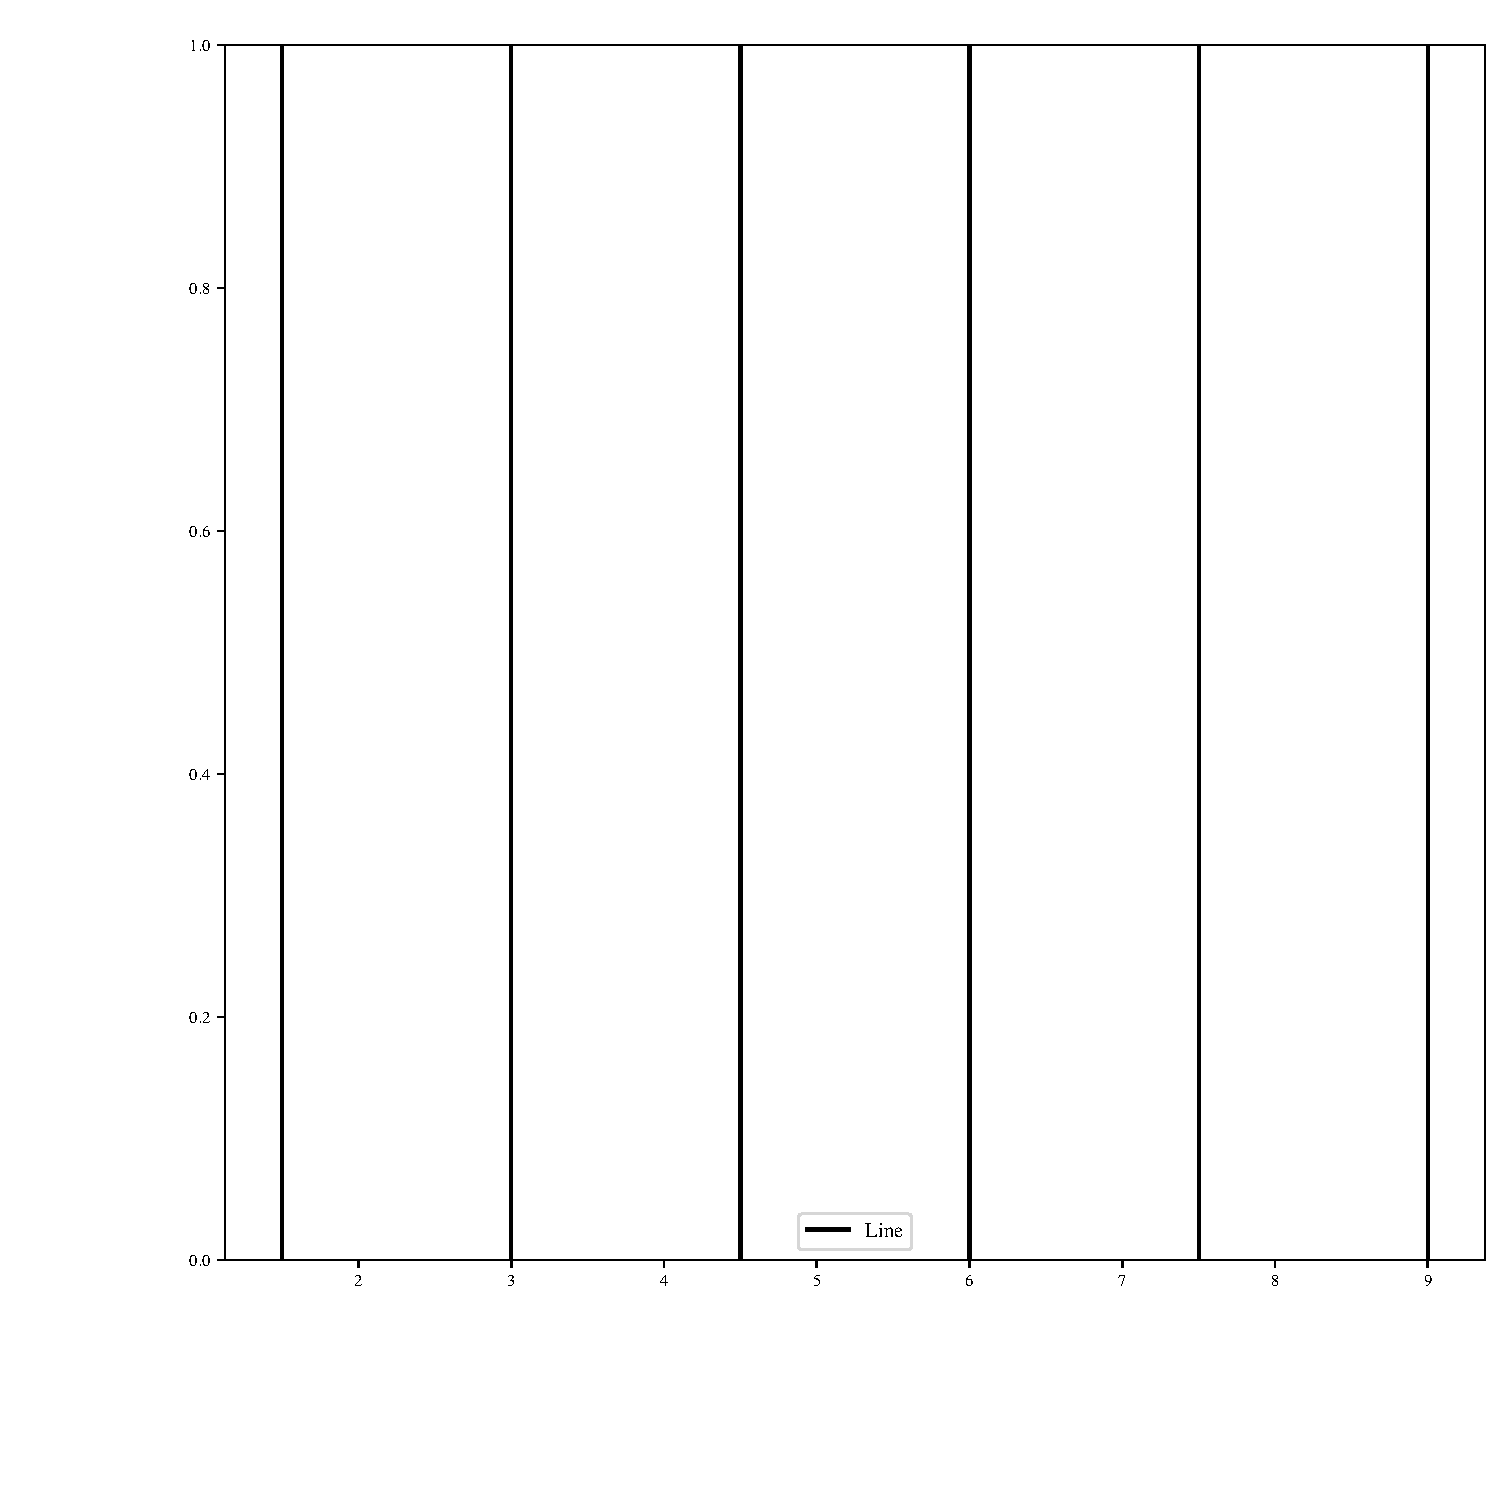
\includegraphics[width=.65\textwidth]{buffon.pdf}
\caption{Sample Buffon needle experiment. 100 needles are dropped on a 10 $\times$ 10 cm area with lines spaced 1.5~cm apart. If a needle lands on a line it is recorded and coloured blue, else it is red. This simulation gave a value of $\pi$ $\approx$ 3.10.}
\label{fig:buffon-needle}
\end{figure}

There are various different approaches to using the Monte Carlo method to obtain randomly sampled variables.
One analytical way of achieving this is the inverted sampling method.
The inverted sampling method can be summarised by the following steps for drawing a sample $X_i$ from an arbitrary PDF $p(x)$:

\medskip

1. Compute the \gls*{cdf} $P(x)=\int^{x}_{0}p(x')dx'$

2. Compute the inverse $P^{-1}(x)$

3. Obtain a uniformly distributed random number $\xi$

4. Finally, compute $X_i = P^{-1}(\xi)$

\medskip

If a given problem cannot use the inverted sampling method, as it may not be possible to get a PDF or analytically invert the CDF, then the rejection method can be used.
The rejection method is essentially a dart throwing method.
This means that points are drawn and compared to the function.
If the point lies under the function then the point is accepted, if it lies above the function then it is rejected.
For example, if a function, $f(x)$ that does not have an analytical PDF, we can use a PDF $p(x)$ such that $f(x) < cp(x)$ where c is a constant.
Therefore sampling from $p(x)$, and if the sampled point lies under $f(x)$ it is accepted, else it is rejected.
~\Cref{fig:picircle} shows an example of this process.

\begin{figure}[!ht]
    \centering
    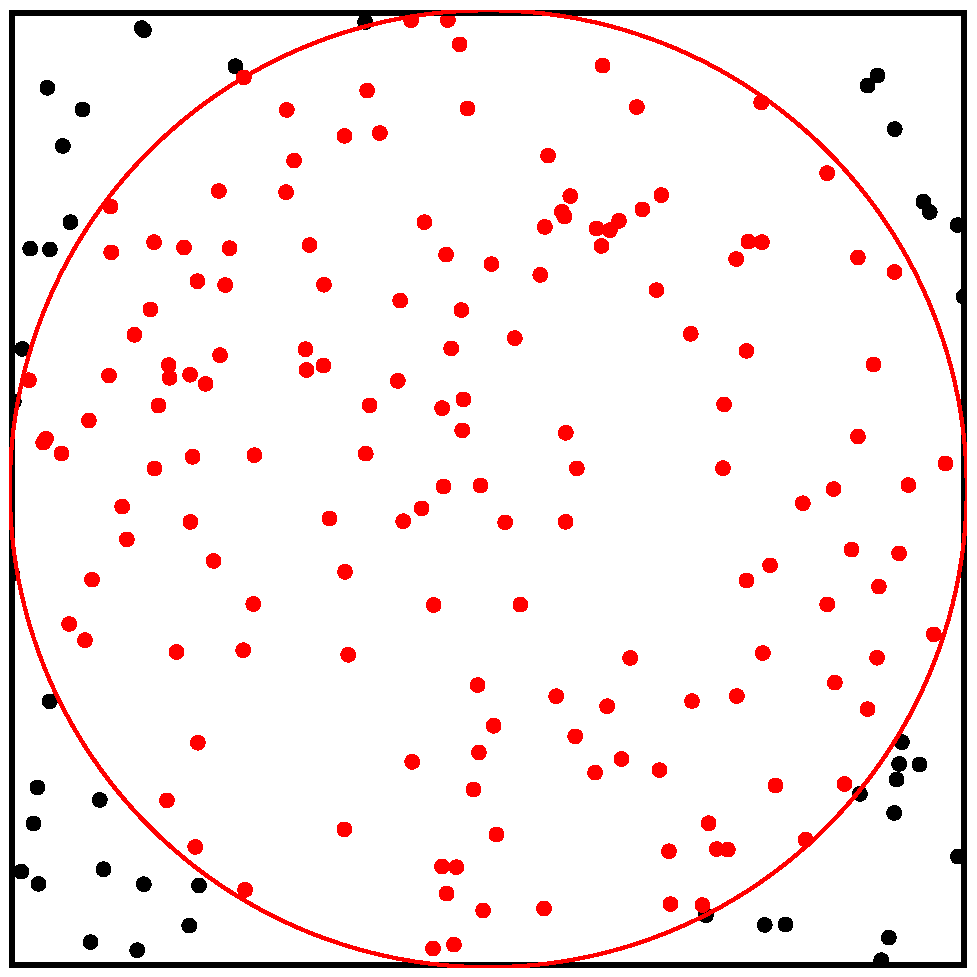
\includegraphics[width=0.35\textwidth]{picirc.pdf}
    \caption{Illustration of the rejection method for determining $\pi$ from the area of a circle inscribed within a square. The ratio of the area of the circle to the square is $\tfrac{\pi}{4}$. Thus the ratio of darts landing in the circle to those that land outside the circle is $\pi \approx \tfrac{4N_{inner}}{N_{total}}$, where $N_{total}$ is the total number of darts, and $N_{inner}$ is the total number of darts that land in the circle. Using 200 darts gave a value of $\pi \approx 3.12$}
    \label{fig:picircle}
\end{figure}


The Monte Carlo method is used in various different disciplines. Ranging from use in the financial sector to analyse investments and stocks by simulating the sources of uncertainty which affect their values~\cite{jackel2002monte,finaceprrof}, use in statistical analysis~\cite{wall2012practical}, and in modern computer generated images (see \cref{fig:ray-trace})~\cite{Kajiyarendering,Cookraytracing}. It is also widely used in astronomy~\cite{robitaille2011hyperion,harries2014torus} and medicine~\cite{valentine2011monte,campbell2015monte}, in order to simulate the propagation of radiation through scattering (turbid) media. This technique, \gls*{mcrt}, is what makes up the bulk of this thesis and is described in depth in the following sections.

\begin{figure}[!htb]
\centering
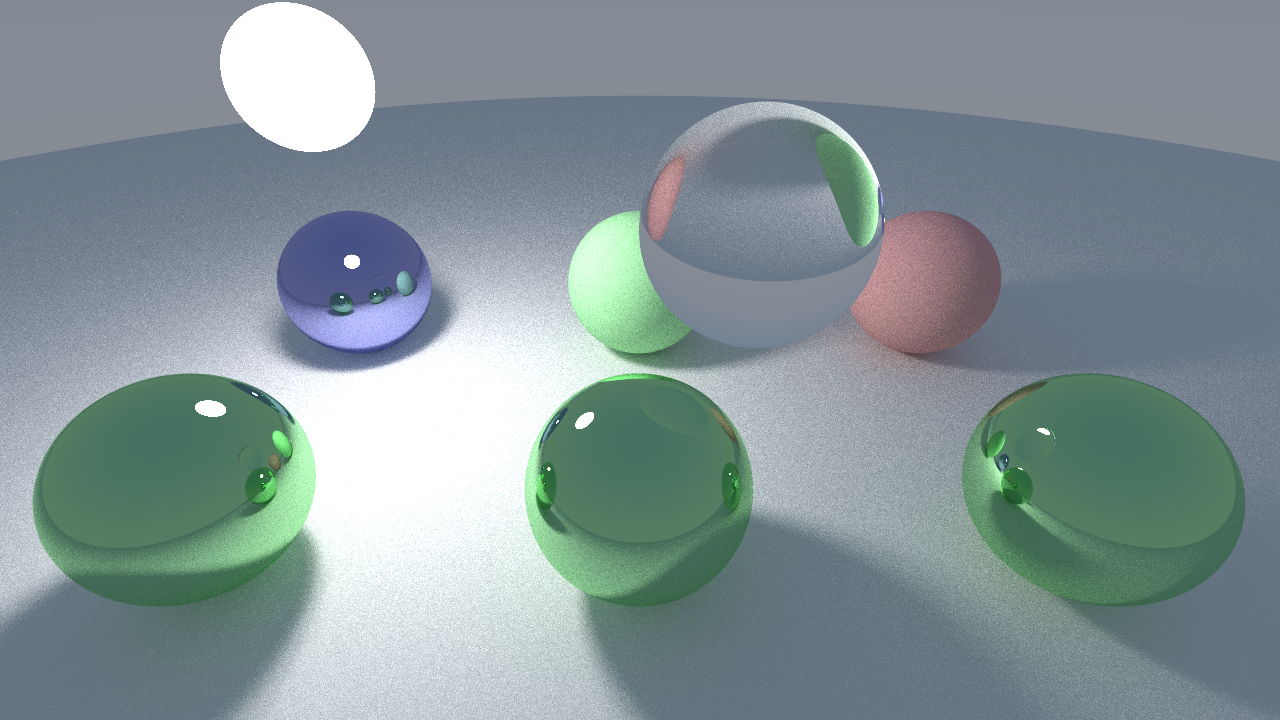
\includegraphics[width=.75\textwidth]{ray-tracing.png}
\caption{Computer generated imagery using ray tracing. The Monte Carlo method is used to ``compute radiance along ray paths between lights and the camera'', in order to generate CGI images~\cite{pharr2016physically}.}
\label{fig:ray-trace}
\end{figure}
\newpage
%\chapter{Monte Carlo radiation transport technique}
\label{sec:mcrt}
\section{Introduction and Background}
This chapter will provide an overview of the Monte Carlo method and how it is used within the context of \gls{mcrt}. The chapter will then present the details of the MCRT code used as the basis of the subsequent chapters. Validation of this code and details of computational speed up are also presented. Subsequent chapters will expand upon the code for each individual projects needs.

\subsection{Monte Carlo method}\label{sec:mcmethod}
The Monte Carlo method is a numerical analysis technique based upon random numbers, which are used to calculate unknown variables in problems. 

The earliest use of the method is in Buffon's needle experiment of the 18$^{th}$ century~\cite{badger1994lazzarini,beckmann2015history,buffon1785histoire}. Buffon asked the question;

\medskip

``Suppose we have a floor made of parallel strips of wood, each the same width, and we drop a needle onto the floor. What is the probability that the needle will lie across a line between two strips?"

\medskip

The solution to this question is as:
for a needle length \textit{l}, strip separation \textit{s}, and where \textit{x} is the distance from the needle to the closest line. Then using a simple geometrical argument, a needle crosses a strip if $x \leq \tfrac{l}{2} sin \theta$.

$x$ is distributed uniformly in [0, $\tfrac{s}{2}$], and $\theta$ in [0, $\tfrac{\pi}{2}$]. Therefore the probability density function for $x$ is $p(x)=\tfrac{2}{s}$, and $\theta$ is $p(\theta) = \tfrac{2}{\pi}$. The \gls{pdf}, is a function of a variable that gives probability for a variable to a take a given value. The \gls{pdf} is normalised over the whole range of the variable, in this case $x$, and $\theta$.
Thus, as $x$ and $\theta$ are independent variables, giving a joint probability of $p(x,\theta) = \tfrac{4}{s \pi}$.
So the probability of a needle of length l ($l<s$) is:

\begin{equation}
P=\int_0^{\frac{\pi}{2}}\int_0^{\frac{l}{2}sin\theta}\frac{4}{s\pi}dx d\theta = \frac{2 l}{s \pi}\label{eqn:buffon}
\end{equation}


\Cref{eqn:buffon} can be used to carry out a Monte Carlo estimation of pi. A simple rearrangement yields: $\pi = \tfrac{2l}{sP}$ where P is the ratio of needles crossing the line over total number dropped. Laplace was the first to suggest that Buffon's needle experiment could be used to estimate $\pi$~\cite{beckmann2015history}. \Cref{fig:buffon-needle} shows an example of simulation of Buffon's needle experiment.

\begin{figure}[!htb]
\centering
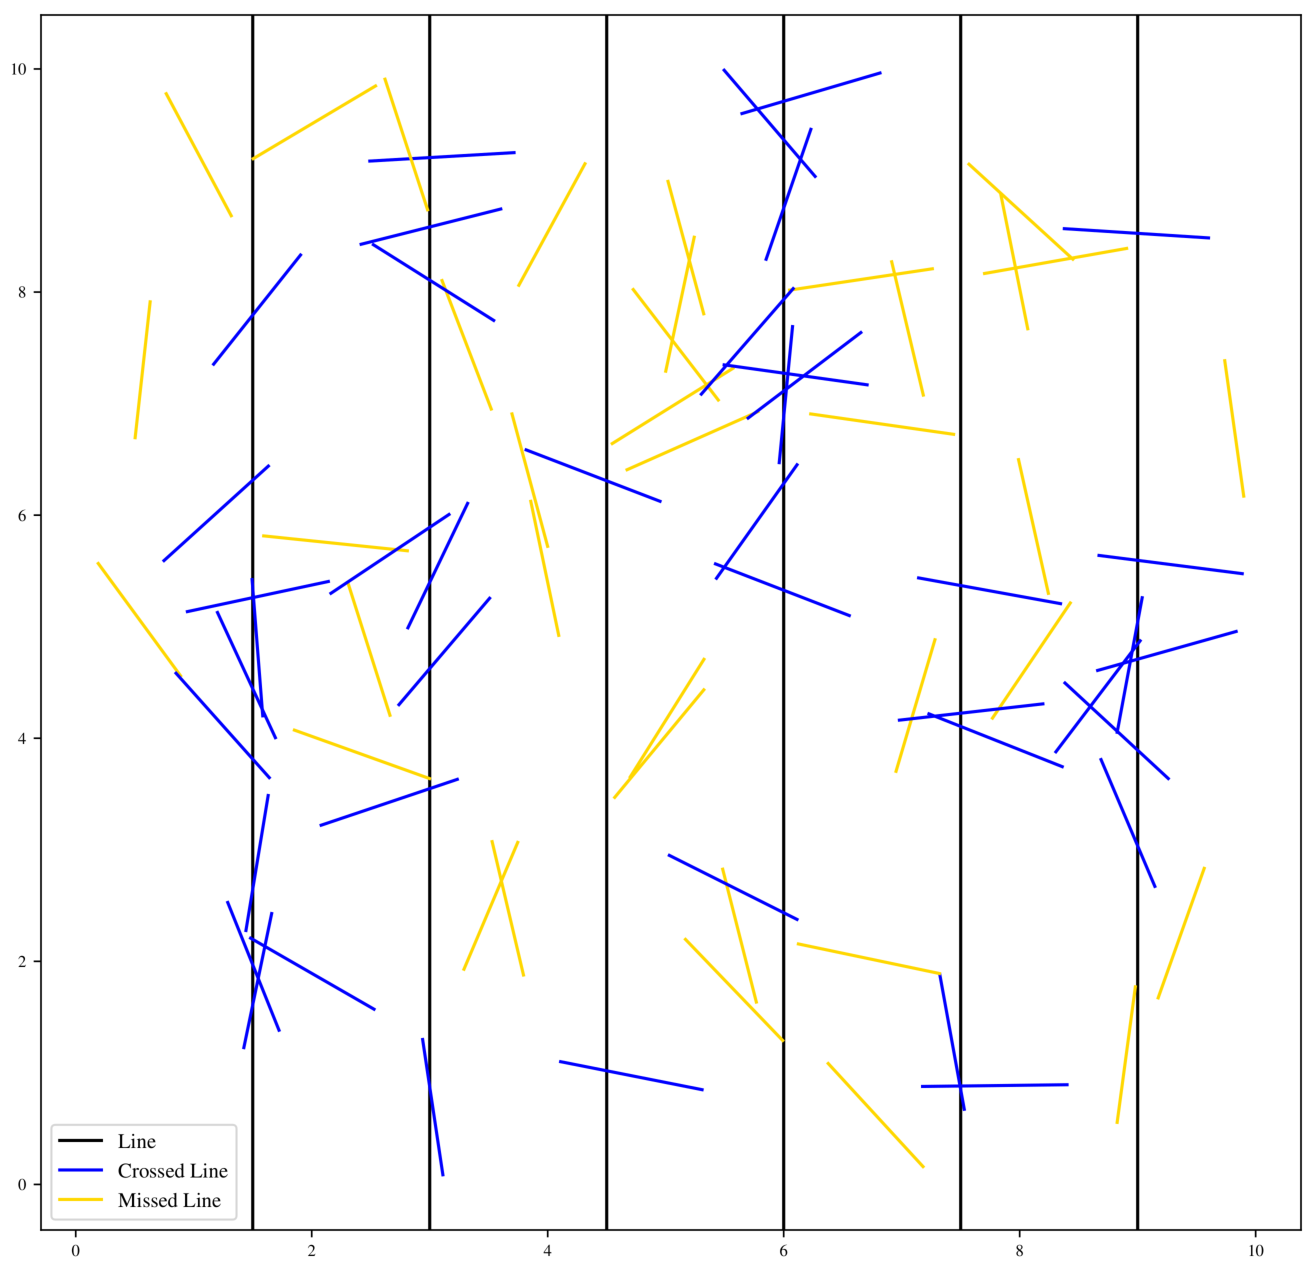
\includegraphics[width=\columnwidth/2]{buffon-pi=317.pdf}
\caption{Sample buffon needle experiment. 100 needles are dropped on a 10 by 10 cm area with lines spaced 1.5cm apart. If a needle lands on a line it is recorded and coloured blue, else it is yellow. This simulation gave a value of pi as 3.17.}
\label{fig:buffon-needle}
\end{figure}

The Monte Carlo method is used in various different disciplines. Ranging from use in the financial sector to analyse investments and stocks by simulating the sources of uncertainty which affect their values~\cite{jackel2002monte,finaceprrof}, use in statistical analysis~\cite{wall2012practical}, and in modern computer generated images (see \cref{fig:ray-trace})~\cite{Kajiyarendering,Cookraytracing}. It is also widely used in astronomy and medicine, in order to simulate the propagation of particles through turbid media. This technique, Monte Carlo radiation transfer, is what makes up the bulk of this thesis and is described in depth in the following sections.

\begin{figure}[!htb]
\centering
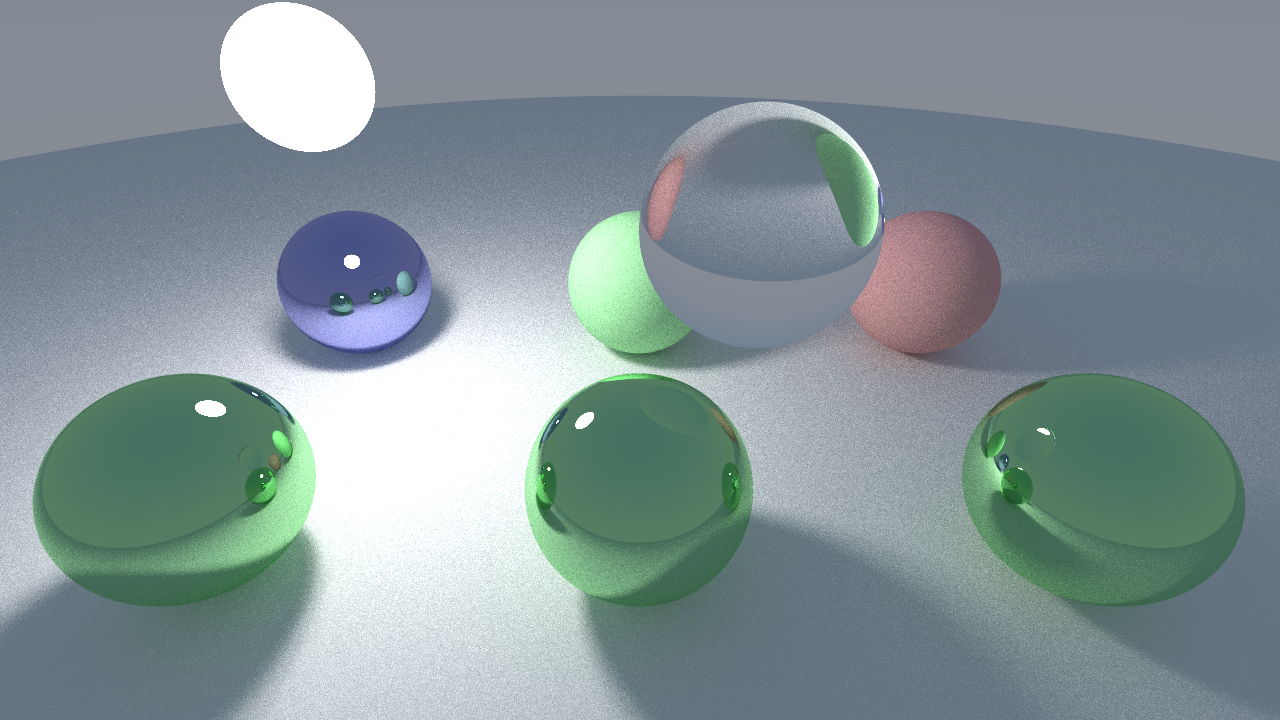
\includegraphics[width=\columnwidth]{ray-tracing.png}
\caption{Computer generated imagery using ray-tracing. Code usd to create image available at: \url{https://github.com/lewisfish/RayTran}}
\label{fig:ray-trace}
\end{figure}
\newpage
\section{Monte Carlo radiation transport algorithm}

\subsection{Introduction \texorpdfstring{$\&$}{and} background}%texorpdfstring supresses warning about pdf bookmarks
The technique that makes up the bulk of this thesis, is the \gls{mcrt} technique. This method was developed at the tail end of the Second World War at the Los Alamos National Laboratory, for the purpose of calculating neutron diffusion though shielding material~\cite{montybeg1,eckhardt1987stan,anderson1986metropolis,ulam1947statistical}. It has since found a myriad of applications from light transport through dusty clouds~\cite{wood1999model}, calculating doses for radiotherapy~\cite{rogers1995beam} to light transport through tissue~\cite{1stmonty}.***more here + link to next section***



\subsubsection{Radiative transfer}
Transport of photons through turbid media, can be modelled analytically using the \gls{rte}. The \gls{rte} models the the radiative losses, and gains by a beam of radiation as it travels through a medium, including: loss of energy due to absorption, loss/gain of energy due to scattering, and energy gain due to emission. Before we derive the \gls{rte}, we first define some terms and physical quantities.


The first term is spectral irradiance, $L_\nu$. Spectral irradiance is defined as the energy flow in a direction \textbf{n}, for a solid angle $d\Omega$, per unit time per unit temporal frequency bandwidth.	
Irradiance is defined as the spectral irradiance over a small frequency range $[\nu, \nu+\Delta \nu]$:

\begin{equation}
	L(\vec{r},\hat{s},t) = L_{\nu}(\vec{r},\hat{s},t)\Delta \nu	
\end{equation}

\noindent Where:

\indent $\vec{r}$ is the position;

\indent $\hat{s}$ is the unit normal vector;

\indent $t$ is the time;

\indent and $L(\vec{r},\hat{s},t)$ is the irradiance [$W \cdot m^{-2}\cdot sr^{-1}$].

\medskip

\begin{figure}[!htb]
	\centering
	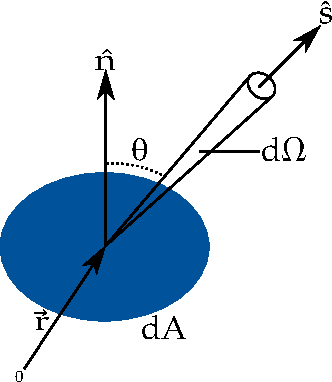
\includegraphics[scale=1.]{diffelement.pdf}
	\caption{Energy flow through area $dA$ within solid angle $d\Omega$ in a direction $\hat{s}$.}
	\label{fig:energydiag1}
\end{figure}

The irradiance can be used to determine the energy, $dE$, transported across an area $dA$, in a solid angle $d\Omega$ in a time $dt$ (see~\cref{fig:energydiag1}) is:

\begin{equation}
	dE = L(\vec{r},\hat{s},t) \cdot (\hat{s} \cdot \hat{n})\ dAd\Omega dt
\end{equation}

\noindent Where:

\indent $\hat{n}$ is the unit normal to $dA$;

\indent and $\hat{s}\cdot\hat{n}$ is the angle of the solid angle.

\medskip

Irradiance can also be used to determine the fluence rate, $\phi$, which is defined as the energy flow per unit time, independent of the flow direction.

\begin{equation}
	\phi(\vec{r},t)=\int_{4\pi}L(\vec{r},\hat{s},t)\ d\Omega
\end{equation}

\noindent Where:

\indent $\phi$ is the fluence rate [$W \cdot m^{-2}$].

\medskip

Irradiance is also the main variable in the \gls{rte}, as it describes the light distribution throughout the medium, and by solving the \gls{rte} yields the irradiance, which in turn gives information on the state of the system and all the physical properties of it.

With the irradiance defined, as well as the other quantities that follow, we can now derive the \gls{rte}. We first consider conservation of energy, as shown in~\cref{eqn:enegyconvo}.

\begin{equation}
	dP = -dp_{div} - dp_{ext} + dP_{scatt} + dP_{src}
	\label{eqn:enegyconvo}
\end{equation}

\noindent Where:

\indent $dP$ is the total change in energy in the volume $dAds$ within the solid angle, $d\Omega$, per unit time (see~\cref{fig:energydiag2});

\indent $dP_{div}$ is the energy loss due to the divergence of the radiation beam per unit time;

\indent $dP_{ext}$ is the energy loss due to absorption and scattering within $dAdsd\Omega$;

\indent $dP_{scatt}$ is the energy gain due to scattering from $\hat{s}'$ into $d\Omega$ per unit time;

\indent and $dP_{src}$ is the energy gain due to emission within the medium, per unit time.

\medskip

The total change in energy in the volume element within the solid angle $d\Omega$, $dP$, is equal to:

\begin{equation}
	dP=\frac{1}{c}\frac{\partial L(\vec{r},\hat{s},t)}{\partial t}\ dAdsd\Omega
	\label{eqn:p}
\end{equation}

\noindent Where c is the speed of light.

\medskip

The first loss term, $dP_{div}$, is the energy loss due to divergence of the radiation beam. This is modelled as:

\begin{align}
	dP_{div}&=\frac{\partial L}{\partial s}\ d\Omega dV \\
		    &=\hat{s} \cdot \nabla L(\vec{r},\hat{s},t)\ d\Omega dV
    \label{eqn:pdiv}
\end{align}

$dP_{ext}$ is the second loss term, and accounts for energy loss due to scattering and absorption in the volume element within the solid angle $d\Omega$. This is modelled as:

\begin{equation}
	dP_{ext}=\mu_t ds\ L(\vec{r},\hat{s},t)\ dAd\Omega
	\label{eqn:pext}
\end{equation}

The first energy gain term, $dP_{src}$, is due to emission in the volume element within the solid angle $d\Omega$. 

\begin{equation}
	dP_{src}=S(\vec{r},\hat{s},t)\ dVd\Omega
	\label{eqn:psrc}
\end{equation}

The second energy gain term, and final term, is due to the incident energy on the volume element within the solid angle $d\Omega$ in direction $\hat{s}$ due to scattering from any direction $\hat{s}'$.

\begin{align}
	dP_{scatt}&=N_sdV\left(\int_{4\pi}L(\vec{r},\hat{s}',t)P(\hat{s}',\hat{s})\sigma_s\ d\Omega' \right)\ d\Omega \\
			  &=\mu_sdV\left(\int_{4\pi}L(\vec{r},\hat{s}',t)P(\hat{s}',\hat{s})\ d\Omega' \right)\ d\Omega 
			  \label{eqn:pscatt}
\end{align}

\noindent Where:

\indent $N_s$ is the number density of scatters;

\indent $P(\hat{s}',\hat{s})$ is the scattering phase function (see~\cref{sec:optprop} for further discussion);

\indent and $\sigma_s$ is the cross section of the scatters, thus $\mu_s=N_s\sigma_s$ (again see~\cref{sec:optprop} for further discussion).

\medskip


Finally substituting~\cref{eqn:pext,eqn:psrc,eqn:pdiv,eqn:pscatt,eqn:p} into~\cref{eqn:enegyconvo} yields the \gls{rte}:

\begin{equation}
\frac{1}{c}\frac{\partial L(\vec{r},\hat{s},t)}{\partial t} + s\cdot \nabla L(\vec{r},\hat{s},t)=-\mu_tL(\vec{r},\hat{s},t)+\mu_s\int_{4\pi}p(\hat{s},\hat{s}')L(\vec{r},\hat{s}',t)d\Omega' + S(\vec{r},\hat{s},t)
\label{eqn:rte}
\end{equation}

\begin{figure}[!htb]
	\centering
	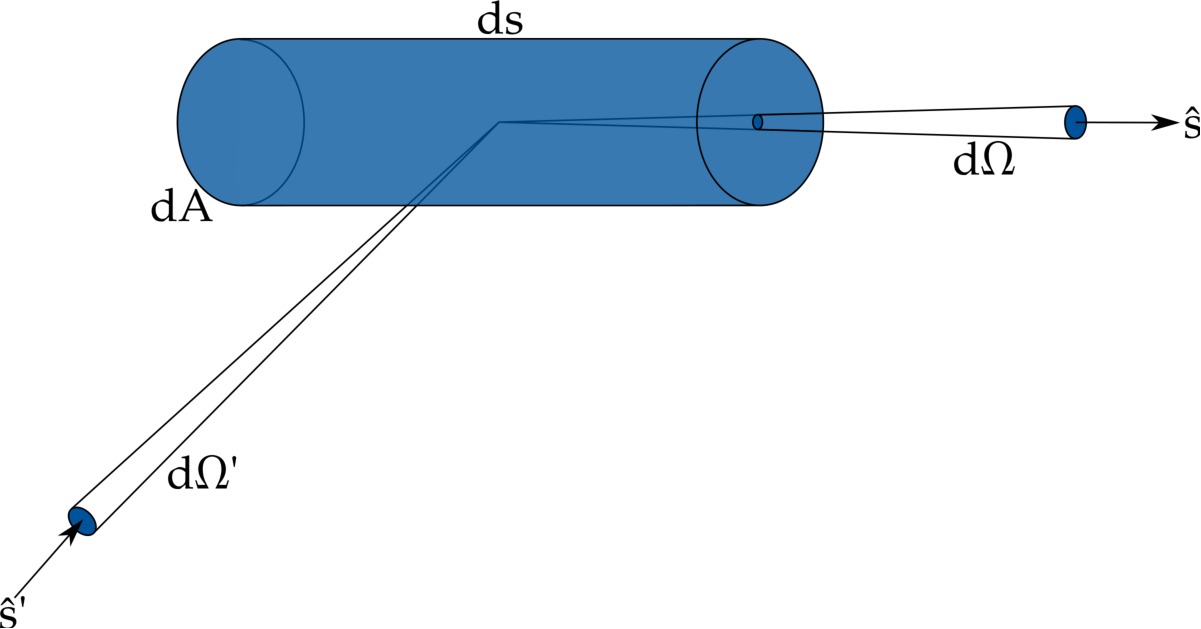
\includegraphics[scale=0.75]{cylinderelement.pdf}
	\caption{Cylindrical volume element, $ds \cdot dA$, with solid angle $d\Omega$ in direction $\hat{s}$ and solid angle $d\Omega'$ in direction $\hat{s}'$. Energy flowing through this element is used to derive the \gls{rte}.}
	\label{fig:energydiag2}
\end{figure}



In general, the \gls{rte} is hard to solve in arbitrary 3D geometries, however there are a number of approximations, and numerical methods available. Diffusion approximation, \gls{km}, and \gls{mcrt} are the common methods used to approximate the \gls{rte}.

\paragraph{Kubelka-Munk theory}
\gls{km} was originally developed in order to calculate the light distribution in thin layered materials, such as paint or paper. The theory is rather simple and makes many assumptions about the medium and the incident light. The main assumptions of \gls{km} are: only scattering and absorption take pace in the medium, the incident light is already diffuse, the medium is uniform, only isotropic scattering, no external or internal reflections, and the medium is planar and infinitely wide.

These assumptions make \gls{km}, very poor for modelling light-tissue interactions. This is as in tissue, scattering is not isotropic, but rather forward biased (see~\cref{sec:optprop}). Tissue is rarely, if ever, planar and infinitely wide. Tissue also has some reflections at its external and internal boundaries, due to change in refractive indices. Many medical and biophotonic treatments/methods use laser light which is not diffuse. Finally tissue can also exhibit fluorescence, which \gls{km} is not able to model, along with polarization. 
\Gls{km} does have some positive aspects. It is good at calculating the diffuse reflectance of simple mediums, and can be used to roughly estimate calculations. Though it is not well suited for modelling light-tissue applications.

\paragraph{Diffusion approximation}
The diffusion approximation for the \gls{rte}, is where the irradiance is separated into two components:

\begin{equation}
	L(\vec{r},\hat{s}) = L_c(\vec{r},\hat{s}) +l_d(\vec{r},\hat{s})
\end{equation}
Where $L_c$ is the unscattered contribution, which satisfies Beer's law, and $L_d$ is the diffuse contribution. The $L_d$ component is expanded using Legendre polynomials and truncated. 
The diffusion approximation also has a number of assumptions and restrictions. The main assumption is that scattering dominates over absorption, and that the scattering is nearly isotropic.

Diffusion theory is computationally fast, and simple. However it is poor at modelling light-tissue interactions due to it's assumptions and restrictions, mainly the inaccurate modelling near the boundaries of the medium and its lack of modelling fluorescence and other microphysics.

The Monte Carlo radiation transfer method is a method of numerically solving the \gls{rte}. The \gls{rte} is the equation that governs how light propagates through a medium with sources and sinks.


***diff theory, kubelka-munk, why mcrt***


\subsection{MCRT algorithm}

The \gls{mcrt} algorithm can be as simple as a $\sim$ 20 line program to as complex as needed for the problem at hand. This section will provide a detailed description a simple \gls{mcrt} algorithm for a 3D voxel based grid.

\subsubsection{Grid set-up}\label{sec:photsetup}

The first step of the \gls{mcrt} algorithm is to set-up the grid which acts as the simulated medium. This grid consists of $n \times n \times n$ voxels\footnote{A voxel is a 3D pixel} of which each voxel has it's own optical properties~(see \cref{sec:optprop} for discussion). This allows the medium of interest to be discretised onto a grid, which gives a good approximation of the real-life medium (see~\cref{sec:codefurther} for discussion on this). along with setting up the medium, arrays which store the locations of the voxel walls in each cardinal direction are created for reference in later parts of the code. Once the medium has been set-up photon packets are launched and propagated through the voxel structure.


%\begin{figure}
%\centering
%\caption{test}\label{fig:voxeldemo}
%\end{figure}

\subsubsection{Photon launch}\label{sec:photlaunch}

The initial step (besides medium set-up and other book keeping) of any \gls{mcrt} algorithm is to launch a photon packet. Depending on the source of photon packets for a given simulation, this step varies from simulation to simulation. The general idea of launching a photon packet is that the packet is given an initial direction vector and position (which consists of a physical position and a voxel position)\footnote{all variables given in this section are the same as they are in the code.}:

\begin{align}
	direction &= \begin{bmatrix}
		n_{xp}\\
		n_{yp}\\
		n_{zp}
	\end{bmatrix}\\
	position &= \begin{bmatrix}
		x_p, y_p, z_p\\
	\end{bmatrix}\\
	voxel &= \begin{bmatrix}
		x_{cell}, y_{cell}, z_{cell}
	\end{bmatrix}	 
\end{align}

In order to set the direction vectors, the components of the direction vectors must be first set. The packets position is tracked using a Cartesian coordinate system, however for ease of computation for calculating scattering angles (see~\cref{sec:photscatterabsorb}), the direction vectors are computed in a spherical system thus the direction vectors are: 

\begin{align}
n_{xp} &= sin(\theta) \cdot cos(\phi) \\
n_{yp} &= sin(\theta) \cdot sin(\phi) \\
n_{zp} &= cos(\theta)
\end{align}

$\theta$ and $\phi$ are generated dependant on the photon source used. The individual sine and cosine terms are saved for use in the scattering routines, see~\cref{sec:photscatterabsorb}.

\subsubsection{Photon move}\label{sec:photmove}

The next step in the algorithm is moving a packet to the next interaction point. The probability a packet will interact over a distance $dL$ is $\mu_tdL$, where $\mu_t$ is the interaction probability (see~\cref{sec:optprop}). Thus the probability of travelling $dL$ without any interaction is $1-\mu_tdL$. Therefore over a distance $L$, with N segments of length $L/N$ the probability of travelling $L$ before any interaction:

\begin{align}
P(L) &= (1-\mu_t\frac{L}{N}) \cdot (1-\mu_t\frac{L}{N}) ...\ (1-\mu_t\frac{L}{N}) = (1-\mu_t\frac{L}{N})^N \\
P(L) &= \lim_{N \to \infty}(1-\mu_t\frac{L}{N})^N=e^{-\mu_tL}=e^{-\tau}\label{eqn:pdfdist}
\end{align}

Where $\tau$ is the number of mean free paths over a distance L. We now have a \gls{pdf}, \cref{eqn:pdfdist}, for the distance a packet will travel before an interaction occurs. For this to be of use we need to be able to sample from this \gls{pdf} in order to get a random optical depth. Using the Monte Carlo method described in~\cref{sec:mcmethod}, with $\xi$ as our random variable, we get:

\begin{equation}
\xi=\int_{0}^{\tau}e^{-\tau'}=1-e^{-\tau}\rightarrow \tau=-log(1-\xi)
\end{equation}

As $\xi$ is symmetric about 0.5 we can substitute $1-\xi$ for $\xi$ yielding:

\begin{equation}
\tau=-log(\xi)\label{eqn:taueqn}
\end{equation} 

We now have an optical distance, however we need to convert this into a physical distance so that we can move our photon packet. From our definition of $\tau$ we know that $\tau=\int_0^L\mu_tdS$, and if we have a smooth, homogeneous medium (i.e not a gridded medium) thus 

\begin{equation}
L=\frac{\tau}{\mu_t}\label{eqn:physicaldist}
\end{equation}

Therefore in order to update the packets position is simply:

\begin{align}
x_p &= x_p+L\cdot n_{xp}\label{eqn:update1}\\
y_p &= y_p+L\cdot n_{yp}\label{eqn:update2}\\
z_p &= z_p+L\cdot n_{zp}\label{eqn:update3}
\end{align}

However as the code in this thesis is a 3D gridded Cartesian code, we have to slightly adjust how we move and update the packets position. As stated in~\cref{sec:photsetup}, the medium has been discretised onto a grid, so that each voxel can have a different $\mu_t$, thus~\cref{eqn:physicaldist} becomes:

\begin{equation}
L=\frac{\tau}{\mu_{t,\zeta}}\quad\quad \zeta=(x,y,z)
\end{equation}

with $\mu_{t,\zeta}$ the $\mu_t$ for the $\zeta^{th}$ voxel. The position is then updated as before using~\cref{eqn:update1,eqn:update2,eqn:update3}. The next step in the algorithm is the interaction event, which can consist of either: scattering, absorbing or fluorescing.

\subsubsection{Photon scatter and absorbing}\label{sec:photscatterabsorb}

The first part of this section of the algorithm is to decide what kind of interaction the packet has with the medium. This section will focus on scattering and absorbing with other interaction events left for the chapters that detail these behaviours.
\medskip

To decide whether a packet scatters or absorbs involves `throwing' a random number and comparing it against the albedo. As detailed in~\cref{sec:optprop} the albedo is the scattering probability $a=\tfrac{\mu_a}{\mu_a+\mu_s}$. The random number is compared to the albedo, and if the random number is less than the albedo then the packet scatters, otherwise the packet is absorbed.

\paragraph{Packet absorption}\hspace{0pt}\\
\\
If the interaction event is a photon packet absorption, then the algorithm terminates the photon packets and starts the next photon packet,~\cref{sec:terminator}.

\paragraph{Packet scattering}\hspace{0pt}\\
\\
If the interaction event is a packet scattering, then the packet is scattered into a new direction and the above process are carried out until a termination clause is met, see~\cref{sec:terminator}.

Depending of the medium being simulated, it can either be isotropically scattering or preferentially scattering in a direction. In the case of simulating photon propagation in tissue, tissue is highly forward scattering.

Anisotropy is the degree of deviation in the photon packets path at each interaction event. The measure of anisotropy is the g value, $g$. With $g$ taking any value from $-1$ to $1$, $-1$ is highly backward scattering, $0$ is isotropic scattering and $1$ is highly forward scattering. 


\subsubsection{Termination}\label{sec:terminator}

\subsection{Code details}

This section details the the actual implementation of the \gls{mcrt} algorithm detailed in the previous section, along with any computational necessities and speed ups on the original algorithm.

\section{Validation of MCRT code}
\section{Optical properties}\label{sec:optprop}

Optical properties of a medium are the properties that determine how light is transport though that medium. Usually the optical properties of a medium are defined by four main parameters: the scattering and absorption coefficients ($\mu_s$ and $\mu_a$), the anisotropy coefficient (g), and the refractive index (n). There are several other optical properties the medium can be defined with, however these in general are only used for specific applications, such as Raman cross-sections.

\subsection{Scattering}

The scattering coefficient defines how much a photon will scatter in the medium per distance

\subsection{Anisotropy}

\subsection{Absorption}

\subsection{Refractive index}

\subsection{Other parameters}



\section{Further extensions to the code}\label{sec:codefurther}
%\chapter{Computational modelling of tissue ablation}
%More background on why developing the laser ablation model. 
%What is the medical reason to want this. %What medical procedures are done with laser ablation? 
%What are the outstanding issues/questions that your model can be used to answer? mention pig skin
%Details of laser pulsing. now add this in experimental results section
%Time steps, convergence tests, etc%Time for holes to be drilled by laser.
%Low intensity damage%in equation 9, could A and Delta-E be functions of temperature?
\section{Introduction and background}%*********************************************************************************************************************************************************
Lasers are used in wide variety of medical procedures not limited to: coagulating scalpels, port wine stain removal, tattoo removal, hair removal, and skin rejuvenation~\cite{amini2010ultrafast, tan1989treatment,kuperman2001laser,liew2002laser,hardaway2002nonablative}.
One class of laser used in these procedures are ablative lasers. Ablative lasers are usually high powered lasers targeted at a specific chromophore in the skin, to partially or fully remove layers of skin. These types of lasers are commonly used for aesthetic procedures such as: skin rejuvenation~\cite{hardaway2002nonablative}, and removal of various diseases such as Rhinophyma~\cite{shapshay1980removal} or lesions/nodules~\cite{valcavi2010percutaneous}. They have also recently been investigated as a means of better drug delivery in the skin for \gls{pdt} treatments~\cite{haedersdal2010fractional}.

One downside to using lasers to remove tissue, it that unlike a scalpel, where the surgeon has full control of the depth of the incision, ablative lasers are not as predictable. Lasers can also cause  unwanted thermal damage to the surrounding areas, leading to unwanted effects.

 Currently the only reliable method to measure the depth of the ablative holes, is via a biopsy, which is an invasive procedure. We propose to use \gls{oct} to measure the ablative crater non-invasively \textit{in-vivo}. The \gls{oct} measurements are then backed up by a computational model. This computational model could then be used to predict the depth of the ablative crater when using a certain power for various different applications such as: laser assisted drug delivery, and various cosmetic applications.

This chapter examines using \gls{mcrt} techniques coupled to a heat transfer simulation, in order to study the thermal damage to tissue due to fractional lasers. Fractionated ablative lasers  are ablative lasers where the power is spread over several beams, such as to leave viable tissue around zones of damaged/necrotic tissue~\cite{manstein2004fractional}. We present experimental work carried out by our collaborators at the University of Dundee and the photobiology department at Ninewells hospital, along side our computational model of tissue ablation.

\section{Methods}

In order to replicate the experimental work \textit{in silico}, our numerical model has three main portions. The first is the \gls{mcrt} that models light transport through tissue so that we can calculate the laser energy deposited as a function of time and space. The second, a \gls{fdm} which is used to calculate the heat diffusion within the tissue due to the absorbed laser energy. Finally, a tissue damage model to track the damage to the tissue caused by the laser. All these individual portions are connected together to create our numerical model. Each portion of the numerical model is described below in more detail.

\subsection{Monte Carlo radiation transport (MCRT)}%**************************************************************************************************************************************************

*This part is here as it will be needed for paper. probably not needed in chapter though...*
\gls{mcrt} is the `gold standard' for simulating the transport of light through biological tissue~\cite{kong2008efficient}. This is due to its flexibility in modelling non standard geometries, and its ability to model various light sources and micro-physics, such as fluorescence. It uses interaction probabilities and random numbers in order to model the `random walk' that photons undergo in a turbid medium. These `packets' can undergo go scattering, absorption and various other physical process \cite{yao1999monte,welch1997propagation}. \gls{mcrt} has been used to model light-tissue interactions in many different medical and biophotonic applications \cite{campbell2015monte,boas2002three,patwardhan2005monte}. \gls{mcrt} is used here to calculate the energy deposited by the laser, which is then passed to the heat transport simulation.

The tissue medium for the \gls{mcrt} and heat transport simulations is a 3D voxel model (\cref{fig:voxel-model}). This allows the variation of optical and thermal properties from voxel to voxel, making it the ideal type of grid for modelling tissue ablation. We use  80 x 80 x 80 voxels *still changing this*, representing a tissue sample size of 1.1 $\times$ 1.1 $\times$ 0.5 cm. We assume the porcine skin is uniform, so that initially our voxel model is uniform, and the optical properties of porcine skin at the wavelength of interest is mainly that of water mixed with protein, see \cref{fig:waterabsor}.


\begin{figure}
\centering
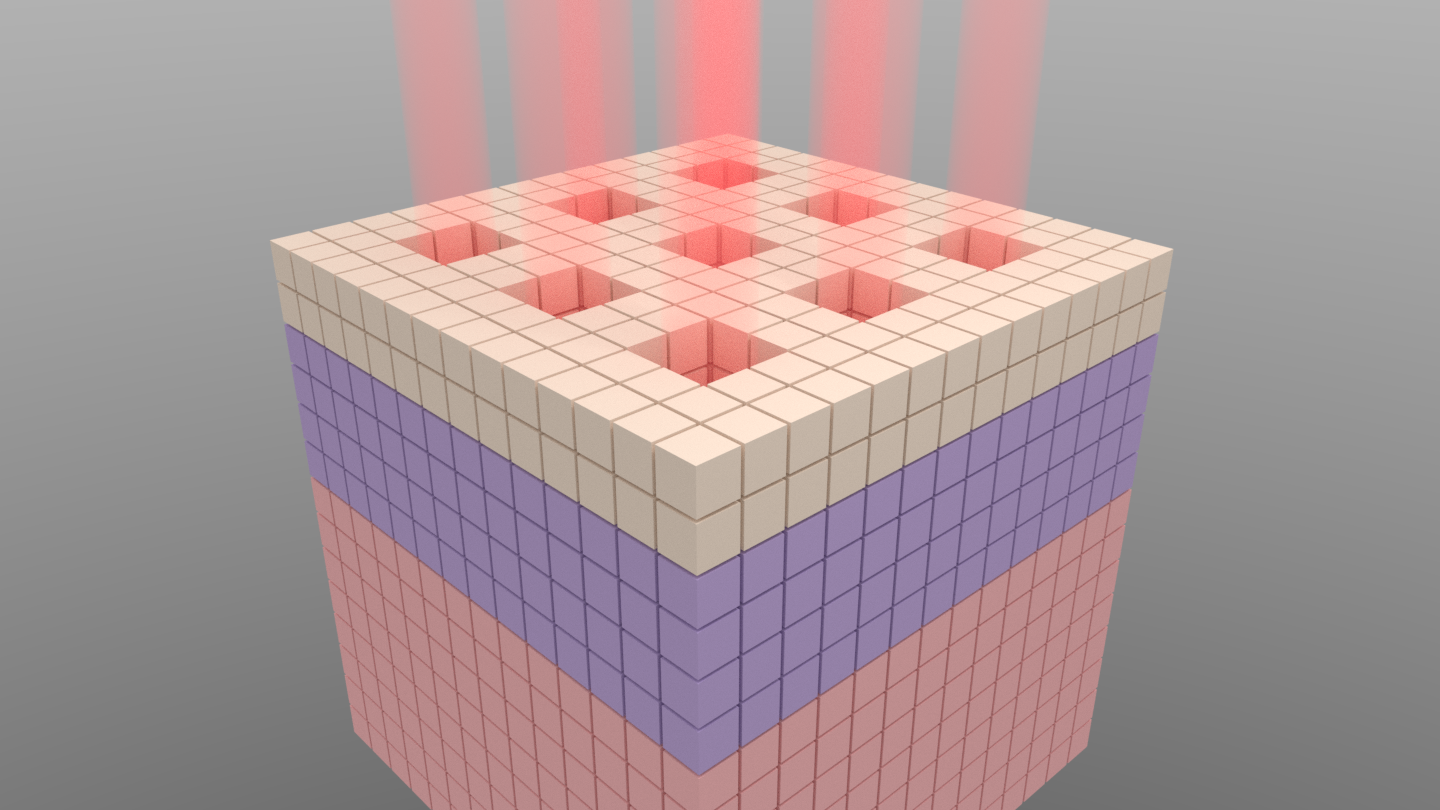
\includegraphics[scale=0.25]{./ablation/images/voxel-model-render.png}
\caption{Example of a possible voxel model, with three different layers, various holes due to ablative pixel beam lasers. Each voxel represents a different optical/thermal propertty of the tissue medium.}\label{fig:voxel-model}
\end{figure}

The original \gls{mcrt} code was developed for astronomy applications \cite{wood1999model,wood2005estimating}, and has since been adapted for medical applications~\cite{campbell2015monte,barnard2018quantifying}.

\Cref{fig:algo}. shows the overall algorithm for the simulation, including the \gls{mcrt} portion. 
The \gls{mcrt} portion of the algorithm begins with determining where the photon enters the medium. This is calculated by randomly selecting one of the pixel beams, from the 9 x 9 array of pixel beams. Next the position on the surface of the medium is calculated. As the profile of the pixel beams are unknown, they are assumed to be uniformly circular *maybe change to gaussian??*. Thus, the packets position is uniformly sampled on a circle the width of the pixel beam.

Once the packet enters the simulation, a propagation distance for the packets is calculated using \cref{eqn:propdist}. The packet then moves this distance before undergoing an interaction event. This can be either scattering or absorption, however in this simulation absorption dominates, and thus we assume no scattering takes place. This process is repeated until the photon has either been absorbed or exits the medium.

\begin{equation}
L = -\tfrac{ln(\xi)}{\mu_a}
\label{eqn:propdist}
\end{equation}

\noindent Where:

\indent $\xi$ a random number ($\tau = -ln(\xi)$, $\tau$ is the optical depth);

\indent $\mu_a$ is the absorption coefficient;

\indent L is the physical distance.

\medskip

\Cref{eqn:propdist} is the equation for a uniform medium. As the medium we are simulating changes over time due to thermal damage this equation has to be adapted for a 3D Cartesian grid. Each voxel 
can have different optical properties, thus the photon packet is moved on a voxel by voxel basis. To start the movement process, a random number is generated, which is used to sample an optical depth the photon packet will travel. Next the photon enters the voxel and the maximum distance the photon can travel in the new voxel is calculated along the photons trajectory. If this optical distance is less than the optical depth sampled, then the photon enters the next voxel. If the distance is larger than the sampled optical distance then the photon has an interaction event in that voxel. The photon packet moves to the interaction event in the voxel and then undergoes scattering or absorption. The whole process is repeated until the photon `dies' via absorption or leaving the medium.
This in turn is again repeated for all the photons, until all the photons have been absorbed or have escaped the tissue medium. We use 1 million photons per \gls{mcrt} simulation run.

\begin{figure}
\centering
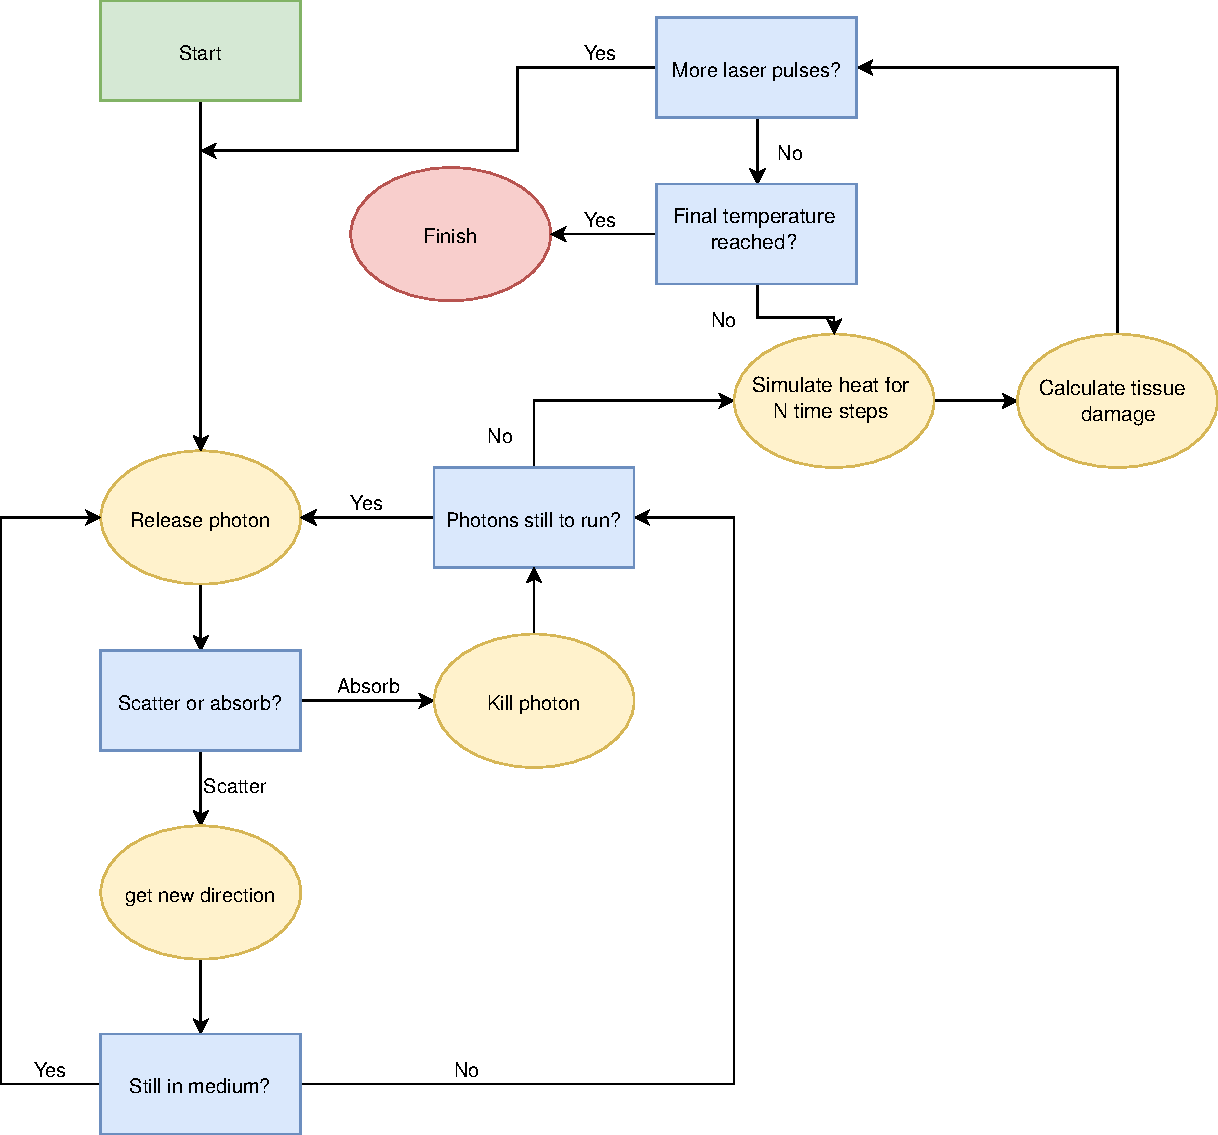
\includegraphics[scale=0.5]{./ablation/images/flowchart.pdf}
\caption{Flowchart of the tissue ablation algorithm.}
\label{fig:algo}
\end{figure}

To calculate the energy absorbed in the porcine tissue via the laser we use the path length counter method devised by Lucy \cite{lucy1999computing}. Thus energy absorbed per voxel is calculated as:

\begin{equation}
E_{i}^{abs} = \frac{L}{N \Delta V_i}\sum\mu_a s
\label{eqn:Eabs}
\end{equation}

\noindent Where:

	\indent L is luminosity [$W$];
	
	\indent N is the number of photons;
	
	\indent $\Delta V_i$ is the volume of the $i^{th}$ voxel [$m^{-3}$];
	
	\indent $\mu_{a,i}$ is the absorption coefficient of the $i^{th}$ voxel [$cm^{-1}$];
	
	\indent and s is the pathlength of a photon packet through the $i^{th}$ voxel [$cm$].
	
	\medskip
	
\begin{figure}
\centering
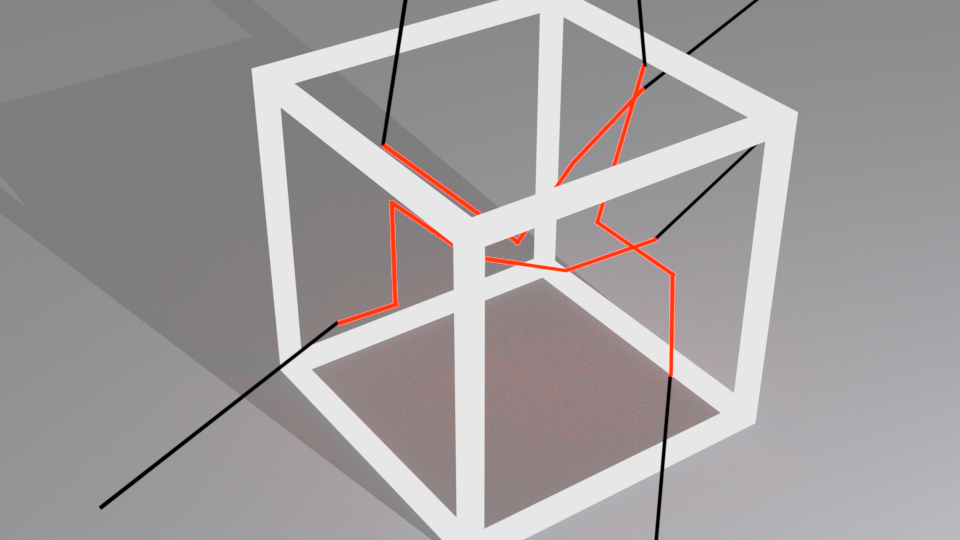
\includegraphics[scale=0.25]{./ablation/images/jmea-explain.png}
\caption{Red lines are photon paths within a voxel. Black lines photon paths outwith the voxel. Red photon paths are summed up in order to calculate the absorbed energy within each voxel.}
\label{fig:jmea-explain}
\end{figure}	
		
This grid of absorbed energy is then passed to the heat transport portion of the simulation, so that the heat diffusion can be calculated.

\subsection{Heat transport}%************************************************************************************************************************************************************************

In order to model the transport of heat in porcine skin, we use the standard parabolic heat equation:

\begin{equation}
\rho c_p \frac{\partial T}{\partial t}= \nabla \cdot (\kappa \nabla T) + \dot{q}
\label{eqn:heat}
\end{equation}

\noindent Where:

	\indent $T(x, y, z, t)$ is the temperature as a function of time and space [\textit{K}];
	
	\indent $\kappa$ is the thermal conductivity [$W\cdot m^{-1}\cdot K^{-1}$];
	
	\indent $\rho$ is the density [$Kg \cdot m^{-3}$];
	
	\indent $c_p$ the specific heat capacity [$J\cdot K^{-1}$];
	
	\indent $\dot{q}(x,y,z,t)$ is the source/sink term as a function of time and space [$W\cdot m^{-3}$].
	
	\medskip

As we are modelling a dynamic system, where the tissue's optical and thermal properties change as a function of space and time, we cannot make the assumption that $\kappa, \rho, \text{and}\  c_p$ are constant and thus we have to solve the non-linear heat equation (\cref{eqn:nonlinearheat}).

\begin{equation}
\frac{\partial T}{\partial t} = \frac{1}{(\rho c_p)_{\xi}}(\nabla k_\xi T + k_\xi\nabla^2T)+\dot{q}\quad \xi=(i,j,k)
\label{eqn:nonlinearheat}
\end{equation}

The $\dot{q}$ term is a heat source/sink term. The heat source in this simulation is due to the laser, and we assume the only loss of heat to the surrounding medium is via convection and conduction.
	
These boundary conditions must be considered. All faces of the cube, bar the laser facing face, are considered to be pinned at 5$^{\circ}$C, as the porcine skin was kept cooled prior to experimental work and the simulation volume is smaller than the porcine tissue samples. The laser facing face has a simple convective BC:	

\begin{equation}
\dot{q}_c = -hA(T - T_\infty)
\label{eqn:bceqns}
\end{equation}

\noindent Where:

	\indent \textit{h} is the heat transfer coefficient [$W\cdot m^{-2}\cdot K$];
	
	\indent \textit{A} is the area of the grid element, that is radiating/convicting heat away [$m^{-2}$];
	
	\indent and $T$, and $T_\infty$ are the temperature in a voxel and the surrounding medium temperature respectively~[$K$].
	
	\medskip

As \cref{eqn:nonlinearheat} is generally hard to solve in arbitrary geometries with complex boundary conditions we employ a numerical method to solve \cref{eqn:nonlinearheat}.
The numerical method we employ is a \gls{fdm}. The \gls{fdm} is derived from the Taylor series approximation for derivatives. A function $f(x)$ is discretised onto a grid with \textit{N} nodes (see~\cref{fig:fdmexplain}). Then at a node \textit{i} we can use the Taylor series approximation in the forward ($+\text{ive}\ x$ direction) and backward ($-\text{ive}\ x$ direction) to give the derivates in~\cref{eqn:fdmfwd,eqn:fdmbck}. Where: \textit{i} is the grid point at $x_o$, $i$+1 is the point at $x_0+\Delta x$, and \textit{i}-1 is the grid point at $x_{o}-\Delta x$. We can then combine these `forward' and `backward' derivatives to give a `central' derivative~\cref{eqn:fdmcent}. We can also give expressions for the $2^{nd}$ order derivatives for backward, forward and central (forward and backward $2^{nd}$ order equations omitted for brevity)~\cref{eqn:fdmcent2}.

\begin{figure}
  \begin{center}
    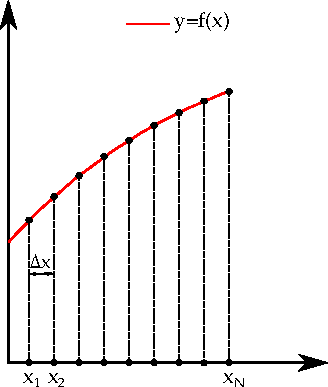
\includegraphics[width=0.48\textwidth]{./ablation/images/fdm.pdf}
  \end{center}
  \caption{Discretisation of \text{f(x).}}\label{fig:fdmexplain}

\end{figure}

\begin{subequations}
\begin{align}
\frac{df}{dx} &= \frac{f_{i+1} - f_{i}}{\Delta x}  &(forward) \label{eqn:fdmfwd}\\
\frac{df}{dx} &= \frac{f_{i} - f_{i-1}}{\Delta x}  &(backward) \label{eqn:fdmbck}\\
\frac{df}{dx} &= \frac{f_{i+1} - f_{i-1}}{2\Delta x}  &(central)\label{eqn:fdmcent}\\
\frac{d^2f}{dx^2} &= \frac{f_{i-1}-2f_i+f_{i+1}}{\Delta x^2} &(central)\label{eqn:fdmcent2}
\end{align}
\end{subequations}


Thus the linear heat equation~\cref{eqn:heat}, in 1D, taking a $1^{st}$ order forward time derivative, and a $2^{nd}$ order central spatial derivative gives:

\begin{subequations}
\begin{align}
\frac{T^{n+1}_i-T^{n}_i}{\Delta t} &= \alpha\frac{T^n_{i-1}-T^n_{i}+T^n_{i+1}}{\Delta x^2}  + \frac{\dot{q}}{\rho c_p}\\
T_{i}^{n+1} &=  \alpha\Delta t \frac{T_{i-1}^n-2T_i^n+T_{i+1}^n}{\Delta x^2} + \frac{\dot{q}}{\rho c_p}
\label{eqn:simplefdm}
\end{align}
\end{subequations}

\begin{figure}
  \begin{center}
    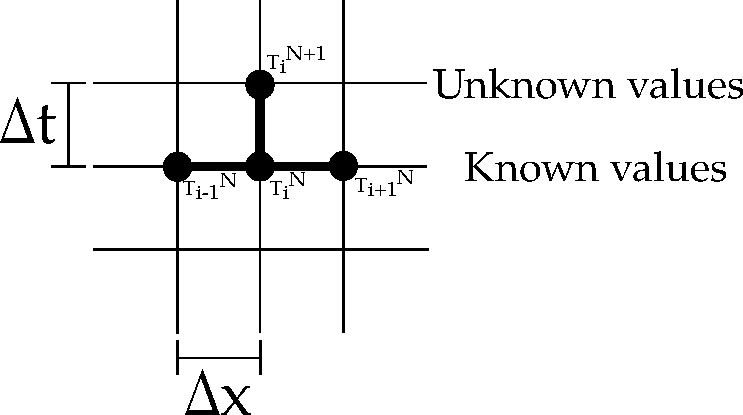
\includegraphics[width=0.48\textwidth]{./ablation/images/fdm-stencil.pdf}
  \end{center}
  \caption{Finite difference method stencil for simple explicit scheme}\label{fig:fdmstencil}
\end{figure}

\Cref{eqn:simplefdm} is called the `simple explicit form of finite-difference approximation'\cite{ozisik1994finite}. \Cref{fig:fdmstencil} shows the `stencil' of this scheme, where there are three known points at time \textit{N}, and just one unknown at time \textit{N+1}. There are various other scheme that can be used to calculate the temperature at the the next time step. However we use a simple explicit scheme here, due to its ease of implementation despite its stability being constrained in comparison to an implicit method. This method is also easily scaled up to 3D with little difficulty.

\medskip

For the more complicated non-linear heat equation we have to account for the change of the medium between points in the space and time. The two easiest methods~\cite{ozisik1994finite} of achieving this is: One, lag the value behind by one step, i.e $c_{p}^{n+1}=c_{p}^{n}$. Two, average $\kappa,\ \rho,\ \text{and}\ c_p$ using a half difference scheme:

\begin{align}
\kappa^{\pm}&=\frac{\kappa_i+\kappa_{i\pm 1}}{2}\\
\rho^{\pm}&=\frac{\rho_i+\rho_{i\pm 1}}{2}\\
c_p^{\pm}&=\frac{c_{p,i}+c_{p,i\pm 1}}{2}
\end{align}

Thus for the simple 1D case as in~\cref{eqn:simplefdm}, we average the thermal properties when computing the coefficients of the temperature nodes, and lag the thermal properties when adding the heat from the laser:

\begin{equation}
T^{N+1}=\Delta t (AT^N_{i-1}-2BT^N_{i}+DT^N_{i+1})+ T_i^N + \frac{\dot{q_L}}{\rho c_p}\label{eqn:heatnonlin1d}
\end{equation}

Where:
\begin{align}
A=&\frac{\kappa^{-}}{\rho^{-}c_{p}^{-}2\Delta x^2} \nonumber \\
B=&\frac{\kappa^{+}}{\rho^{+}c_{p}^{+}2\Delta x^2} \label{eqn:coeffsABD}\\
D=&\frac{(A+B)}{2} \nonumber
\end{align}

\Cref{eqn:heatnonlin1d} can be generalised to higher dimensions easily. The 3D case gives:

\begin{align}
U_{xx} &=  (A T^N_{i-1,j,k} - 2B T^N_{i,j,k} + D T^N_{i+1,j,k}) \label{eqn:FDMheat1}\\
U_{yy} &=  (A T^N_{i,j-1,k} - 2B T^N_{i,j,k} + D T^N_{i,j+1,k}) \label{eqn:FDMheat2}\\
U_{zz} &=  (A T^N_{i,j,k-1} - 2B T^N_{i,j,k} + D T^N_{i,j,k+1}) \label{eqn:FDMheat3}\\
T^{N+1}_{i,j,k} &= \Delta t\ (U_{xx} + U_{yy} + U_{zz}) + T^{N}_{i,j,k} + \tfrac{\Delta t}{\rho c_p}\dot{q_L} \label{eqn:FDMheat4}
\end{align}

\noindent Where:

	\indent $T^{N+1}_{i,j,k}$ is the new temperature at node $i,j,k$ [$K$];
	
	\indent $T^N_{i,j,k}$ is the temperature at node $i,j,k$ at the current time step [$K$];
	
	\indent $\alpha$ is the thermal diffusivity [$m^2\cdot s^{-1}$];
	
	\indent $\kappa$ is the thermal conductivity [$W/m\cdot K$];
	
	\indent $\Delta x\ etc.$ is the size of the grid element in the $p^{th}$ direction [$m$];
	
	\indent and $A, B,D$ are the coefficients in their respective dimension (\cref{eqn:coeffsABD}).

	\medskip
	
Incorporating B.Cs on the top air exposed face:

\begin{equation}
U_{zz} = \tfrac{\alpha}{\Delta z^2} (\tfrac{2 \Delta z}{\kappa} (-h(T^N_{i,j,k}-T^N_\infty) ) -2 T^N_{i,j,k} + 2T^N_{i,j,k+1}) 
\end{equation}

As the lasers *maybe remove s?* operate in a pulsed mode, we account for this in our simulation. We assume that the pulse shape is a top-hat pulse for simplicity. In the heat simulation we have an additional variable in the term $laserOn\cdot\tfrac{\alpha \Delta t}{\kappa}\dot{q_L}$ in \cref{eqn:FDMheat4}. This additional variable, laserOn, is a boolean value, which is defined as:

\[   
laserOn = 
     \begin{cases}
       \text{1,} &\quad\text{if time}\le\text{pulse length}\\
       \text{0,} &\quad\text{if time}>\text{pulse length}.\\
     \end{cases}
\]

In the instance where there is more than one pulse, the laser is turned on and off based upon the pulse frequency.

\medskip

As we are using a simple explicit \gls{fdm}, the time step is constrained in order to make the solution stable. For a cubic 3D \gls{fdm} without prescribed flux BCs, yields the constraint: $\Delta t \leq \tfrac{\alpha \Delta x^2}{2\beta}$. However as we have a flux prescribed boundary condition, the constraint on the time is more severe. Along with this time restraint, the pulse length of the laser also has to be considered. If the time step of the heat simulation is too large it will not account for the heat deposited by the laser. Thus, the timestep has to be an order of magnitude smaller than the shortest laser pulse.

As the timestep is small, and the grid resolution large, the resultant simulation is slow. Thus the code has been fully parallelised to improve performance. Both the \gls{mcrt} and heat simulation are independently parallelised. As discussed in *ref here*, the \gls{mcrt} simulation is fully parallelised, and the results are passed to the heat simulation.

\medskip

Parallelisation of the heat simulation is more involved than the `embarrassingly parallel' class of problems that \gls{mcrt} belongs to. This is due to the heat simulation needing to know the temperature of adjacent nodes. Thus information will have to be passed from each individual core during computation, as opposed to doing the information passing at the end of the simulation \textit{\`a la} \gls{mcrt} parallelisation.
The heat simulation is parallelised using a technique called `halo swapping'. This involves splitting up the computational domain (see \cref{fig:griddecomp}), in this case the tissue medium, and doing the calculations on each domain on a separate core. The `halo swapping' comes in when cores need to communicate with each other about updating their boundary temperature nodes (see \cref{fig:haloswap}).

On a workstation computer these simulations were carried out on (Intel Xeon E3-1245 v5, 8 core @ 3.5GHz) led to a speed up of $\sim$6, over the serial simulation. Using Amdahl's law\cite{amdahl1967validity}, the serial portion of the simulation is $\sim$ 5\%, giving a theoretical speed up $\sim$ 20 times the serial simulation.


\begin{figure}
\vspace{-45pt}
\centering
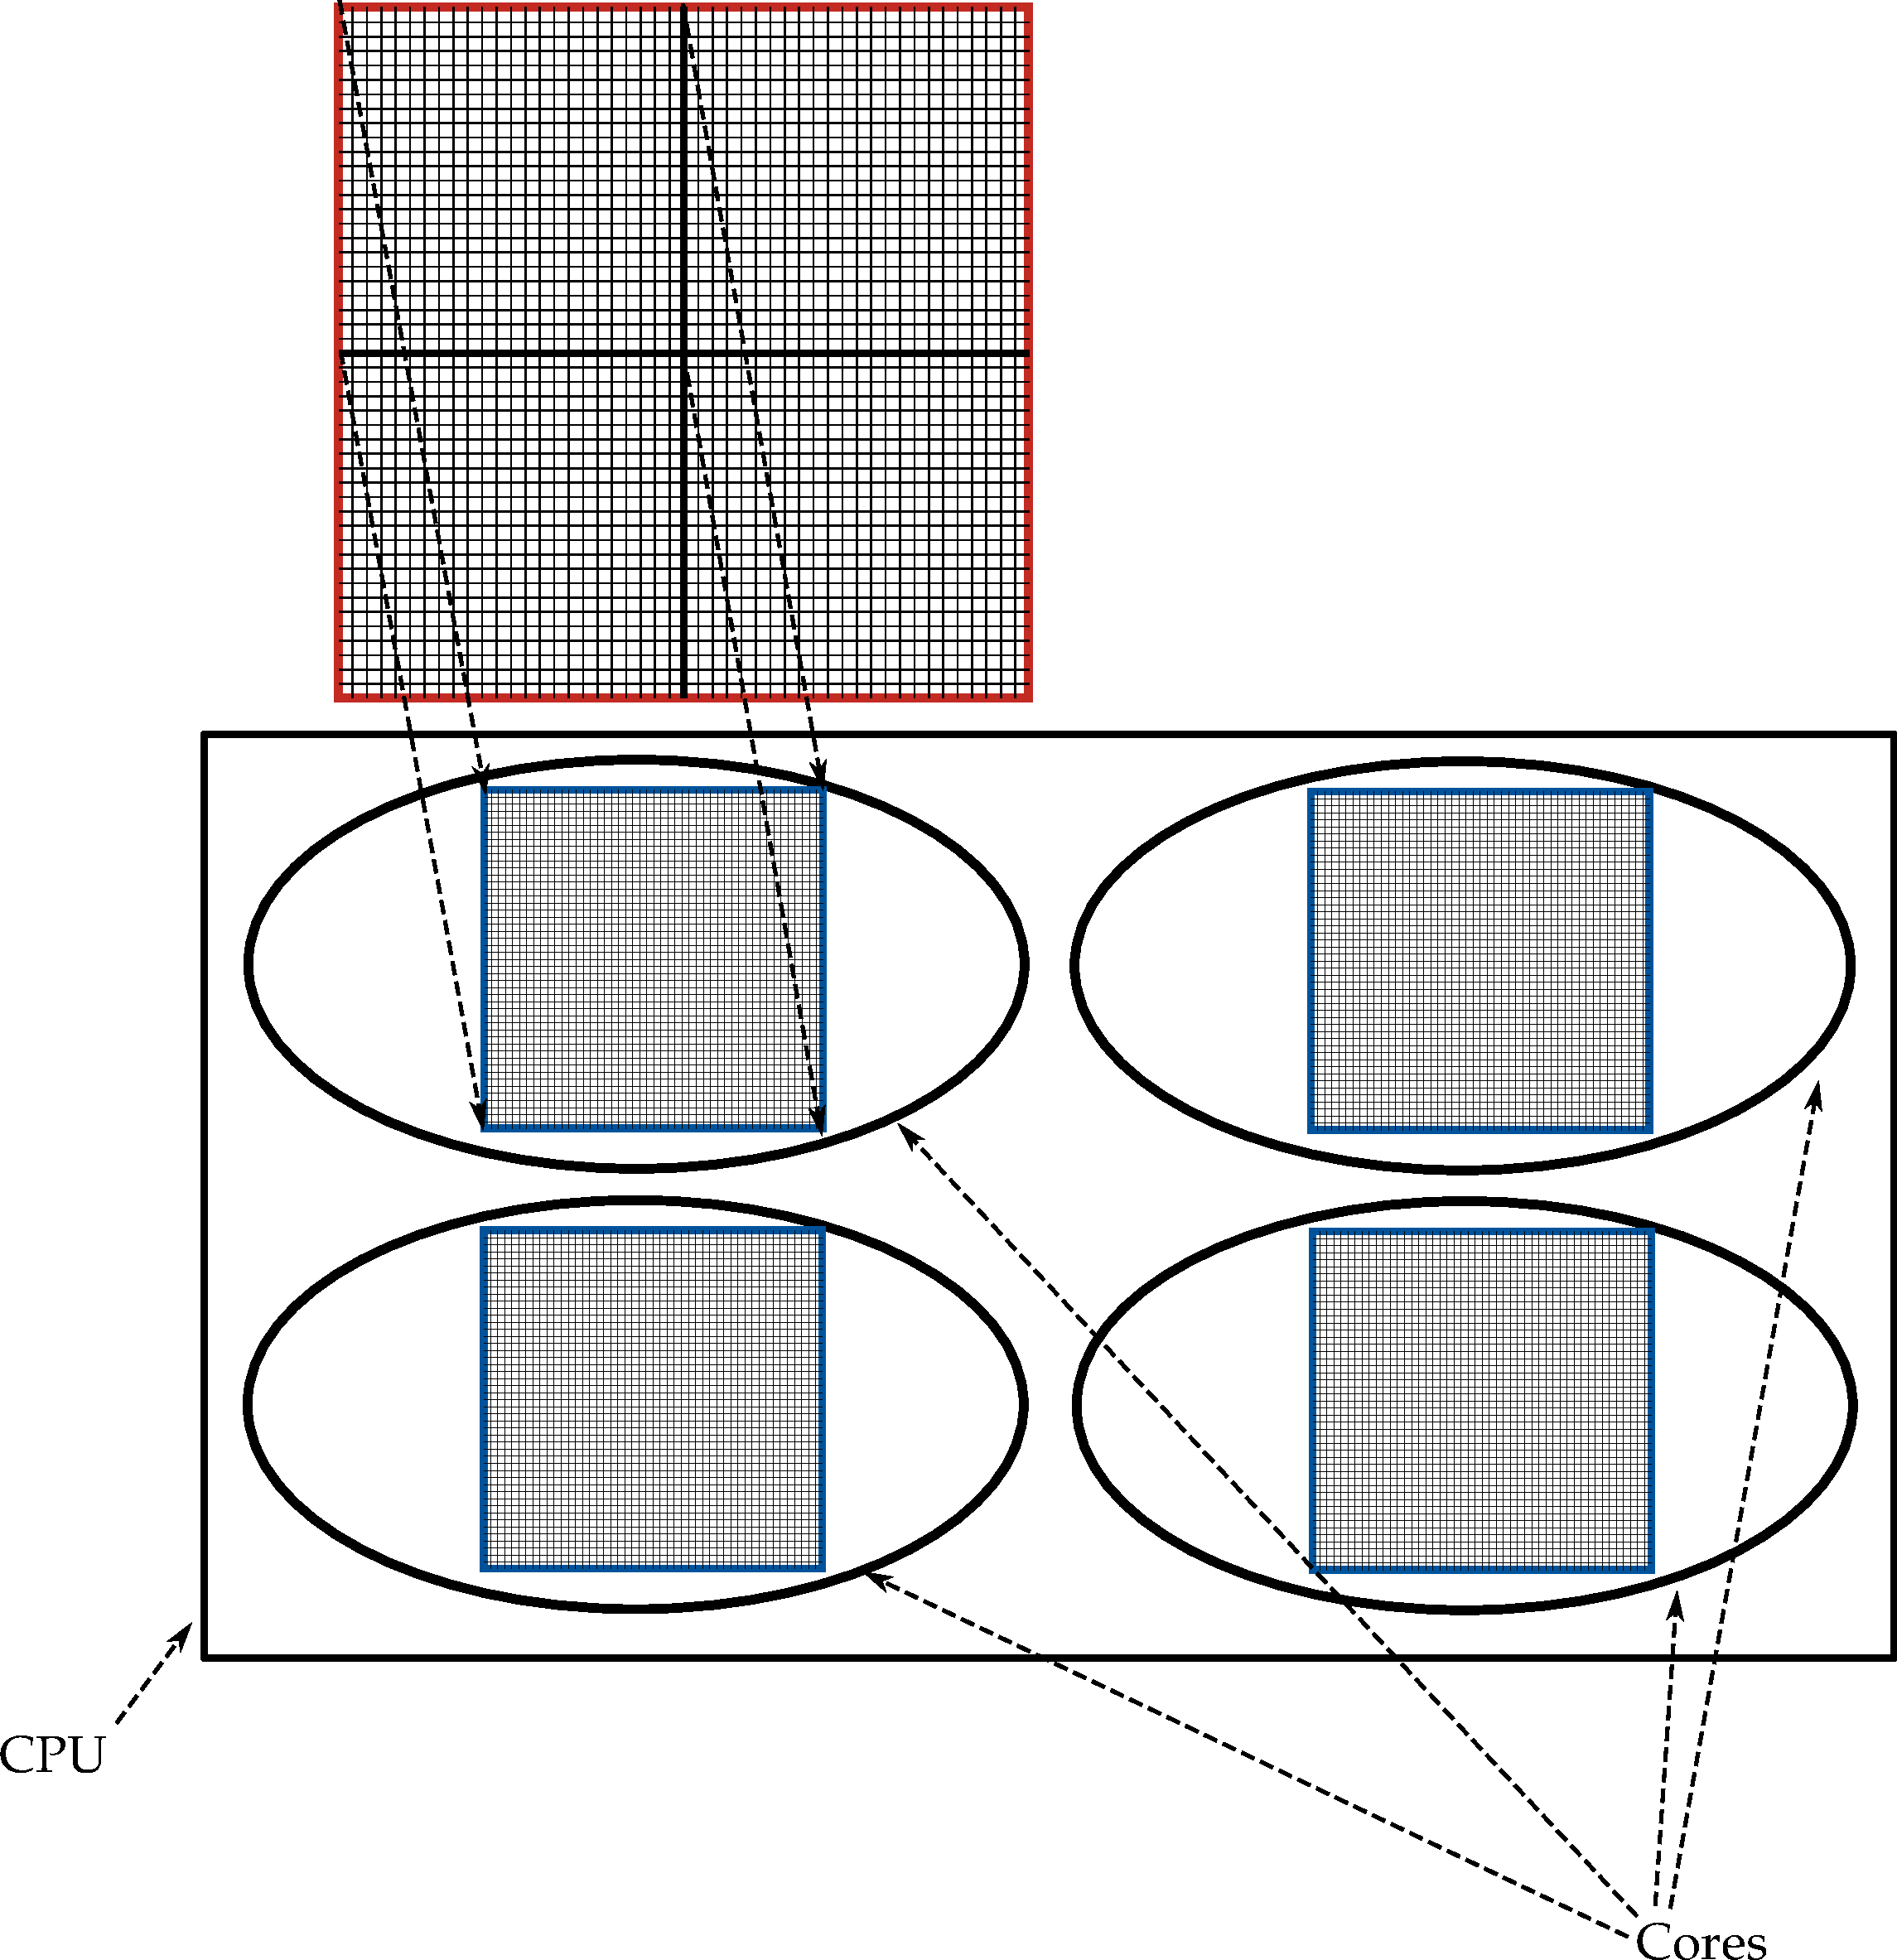
\includegraphics[scale=.35]{./ablation/images/grid-decomp.pdf}
\caption{Computational domain decomposition. Total computational domain is evenly divided between cores in the CPU. This is done via layers of the domain in the z direction. Information is passed to/from cores via the `halo swap' process (see~\cref{fig:haloswap}).}
\label{fig:griddecomp}
\vspace{-10pt}
\end{figure}

\begin{figure}
\centering
\def\svgwidth{350pt}
\input{./ablation/images/halo.pdf_tex}
\caption{Halo swapping. Process A updates the area in red and blue on the left. It updates the blue area which is sent to process B as B's `halo'. Process B cannot update it's own halo, but rather updates the halo for process A.}
\label{fig:haloswap}
\end{figure}


After the heat transport has been completed, the grid of temperatures is passed to the tissue damage portion of the simulation.
\newpage
\subsection{Validation}%************************************************************************************************************************************************************************



\subsubsection{Heat transport validation}

In order to thoroughly validate the numerical method we employ to solve the heat equation, we compare the numerical method against an easily solvable case. We solve the heat equation on a cube, side L, in a surrounding medium of 0$^{\circ}$C. The cube is initially at temperature 37$^{\circ}$C and we calculate the temperature at time \textit{t=0.1s}. Thus the boundary conditions are:

\begin{align}
T(0,y,z,t)&=T(x,0,z,t)=T(x,y,0,t)=0^{\circ}\text{C} \label{eqn:bc1}\\
T(L,y,z,t)&=T(x,L,z,t)=T(x,y,L,t)=0^{\circ}\text{C} \label{eqn:bc2}\\
\end{align}

The thermal diffusivity~($\alpha$), density~($\rho$), and heat capacity~($c_p$) are all set to 1. Assuming a separable solution in Cartesian coordinates for the heat equation yields:

\begin{equation}
\begin{split}
T(x,y,z,t)=&(A_1Cos(\alpha x) + A_1Sin(\alpha x))\cdot\\
&(B_1Cos(\beta y) + B_1Sin(\beta y))\cdot\\
&(C_1Cos(\gamma z) + C_1Sin(\gamma z))\cdot e^{-\alpha\mu^2t}\\
\end{split} 
\end{equation}

\begin{equation}
\mu^2=\alpha^2+\beta^2+\gamma^2
\end{equation}

Applying the boundary conditions (\cref{eqn:bc1,eqn:bc2}) gives:

\begin{equation}
A_1=B_1=C_1=0\
\text{and}\ \alpha=\frac{\pi n}{L}\ \beta=\frac{\pi m}{L}\ \gamma=\frac{\pi p}{L}
\end{equation}

\begin{equation}
\therefore  T_{nmp}(x,y,z,t)=A_{nmp}Sin\left(\frac{\pi n x}{L}\right)\cdot Sin\left(\frac{\pi m y}{L}\right)\cdot Sin\left(\frac{\pi p z}{L}\right)
\end{equation}

This yields the following solution for the heat equation using the principle of superposition, and solving \cref{eqn:heatfactoranalytic} with $f(x,y,z)$ as the initial temperature profile of the cube:

\begin{equation}
A_{nmp}=\frac{8}{L^3}\int_0^L\int_0^L\int_0^L f(x,y,z)\cdot sin(\frac{\pi n x}{L})\cdot sin(\frac{\pi n y}{L})\cdot sin(\frac{\pi n z}{L})\ dx\cdot dy\cdot dz
\label{eqn:heatfactoranalytic}
\end{equation}

\begin{equation}
T(x,y,z,t)=\sum^\infty_{n=1,3,..}\sum^\infty_{m=1,3,..}\sum^\infty_{p=1,3,..}\frac{2368}{\pi^3nmp}Sin(\frac{\pi n x}{L})Sin(\frac{\pi m y}{L})Sin(\frac{\pi p z}{L})e^{(-\lambda^2t)}
\end{equation}

\noindent Where:

	\indent $\lambda^2=\alpha\pi^2(\tfrac{n^2}{L^2}+\tfrac{m^2}{L^2}+\tfrac{p^2}{L^2})$;
	
	\indent $n,m,p$ are odd integers;
	
	\indent and $L$ is the length of the cube.
	
	\medskip
	
At time, $t=0.1$s, a slice through the middle of the cube, $L=1~cm$,  yields \cref{fig:validation-heat}.

\begin{figure}	
\vspace{-10pt}
	\centering
	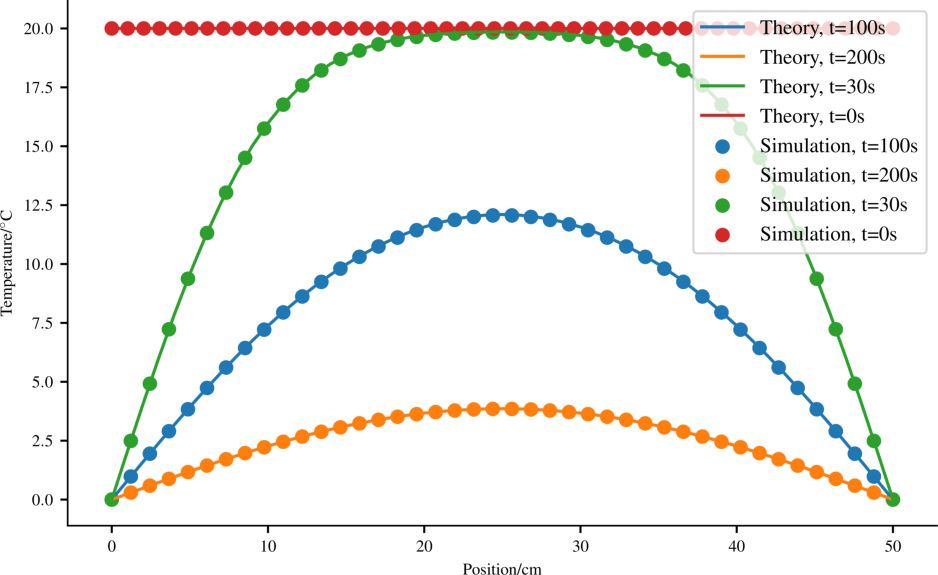
\includegraphics[width=\columnwidth]{./ablation/images/validation.pdf}
	\caption{Comparison between analytical solution and numerical method.}
	\label{fig:validation-heat}
	\vspace{-10pt}
\end{figure}	

\subsubsection{MCRT $\&$ heat transport validation}

As a first test of our code, both \gls{mcrt} and heat simulation, we compare to a simple analytical model of ablation. The simple model of ablation is as this: We define the ablation energy ($E_a$) as the minimum energy required to raise the temperature of the medium to 100~$^{\circ}$C, and then boil off the water in a volume dV, mass M. Thus in 1 dimension we have~\cref{eqn:ablationenergy}, where the symbols have their usual meanings. If the energy for ablation is delivered in a time \textit{dt} by a laser of power density ($Wcm^{-2}$) this gives \cref{eqn:midequationablation}.~\Cref{eqn:midequationablation} can be rearranged in order to give an ablation front velocity, \cref{eqn:ablationvelo}.


\begin{align}
E_a &= c_p \rho dx \Delta T + L_v \rho dx \label{eqn:ablationenergy}\\
P\cdot dt &= \rho dx (c_p \Delta T + L_v) \label{eqn:midequationablation} \\
u &= \frac{P}{\rho(c_p\Delta T+ L_v)} \label{eqn:ablationvelo}
\end{align}

Assuming the ablation front moves with constant velocity during the ablation, and using $L_v=2.53\cdot 10^6\ J\cdot Kg^{-1},\ c_p=4181\ J\cdot Kg^{-1}\cdot K^{-1}$ and the medium is a cube side $2\ mm$, with a starting temperature is 37~$^{\circ}$C with a water content of 70\% giving a density of 700~$Kg\cdot m^{-3}$. For these parameter this gives an ablation velocity, $u\simeq 0.77\ cm\cdot s^{-1}$, and a time to ablate through 2~$mm$ of $t \simeq 0.26~s$.
As the code developed in this chapter simulates the diffusion of heat in a medium due to an incident laser, the expected time to ablate through the same medium should be slightly less as heat diffuses away from the voxel while it is heated being heated. When the full heat + \gls{mcrt} code is used to simulate this experiment, it gives a time, $t \simeq 0.33~s$.	
	
\subsection{Tissue Damage}%************************************************************************************************************************************************************************
\label{sec:tissuedamage}

\subsubsection{Introduction}
The final portion of the simulation is the tissue damage model. To be able to model damage to the tissue we first need to be able to describe the tissue damage process due to heating from a laser.

When the laser is turned on, the temperature starts to rise within the tissue due to the absorption of photons by the tissue. The temperature rise causes damage to the tissue when above a threshold temperature, $T_d$, approximately 43$^{\circ}C$~\cite{welch2011optical}*p539*. From the temperature, $T_d$, we define four main areas of tissue damage:


\begin{equation}
T = 
     \begin{cases}
       \text{coagulation,} &\quad T_d\leq T \leq 100\\
       \text{water boils,} &\quad T=100\\
       \text{carbonisation,} &\quad 100 \leq T \leq T_a\\
       \text{ablation,} &\quad T=T_a.\\
     \end{cases}
\end{equation}


The area of tissue damage we term `coagulation' is a multifaceted process. At 43$^{\circ}$C - 50$^{\circ}$C, bonds break within cell membranes, causing ruptures, and some cell death~\cite{welch2011optical}. This process is usually termed \textit{hyperthermia}. Around 50$^{\circ}$C, enzyme activity decreases, cells become immobile, and various cell repair mechanisms are disabled, leading to more cell death. Temperatures of 60$^{\circ}$C +, proteins become denatured. Thermal denaturation is a structural and functional change in a protein due to the heating it undergoes. This means they change from a highly organised structure with specific purposes, to disorganised structures with no function at all.  A classic example of denaturation of proteins, is in cooking eggs. Denaturation occurs when the clear fluid egg white, rich in protein albumin, becomes a solid white~\cite{niemz2013laser}.

The next stage in the tissue damage process is the vaporisation of water. As the temperature of the tissue starts to approach 100${^{\circ}}$C (at 1 atm), water starts to vaporise. If the vaporised water cannot escape the tissue it forms steam vacuoles, little pockets of steam. These vacuoles can easily been seen when viewing tissue samples after tissue has been treated with a high powered laser (see \cref{fig:histology}). In certain conditions these steam pockets can explode, with these `explosions' being audible by the human ear~\cite{petrella2013popcorn}.


The third stage of tissue damage is carbonisation or carmelisation of the tissue. This occurs when most of the water has boiled off, leaving the remaining tissue to heat up and reduce to its elemental carbon form. This carbonisation of tissue, when it occurs, is generally only a thin layer of 5-20~$\mu m$~\cite{welch2011optical}.

The final stage of tissue damage is the removal of the remaining tissue, i.e tissue ablation. There is no agreement in the literature how tissue undergoes ablation with a number of methods proposed~\cite{vogel2003mechanisms}. The tissue ablation process is not a simple process, with various unknowns which depend on everything from tissue composition to laser power and pulse length. The literature however, does suggest that it takes place when the tissue temperature is between 177 and 500${^{\circ}}$C\cite{gerstmann1994char,mckenzie1986three}.

\begin{figure}	
\vspace{-10pt}
	\centering
	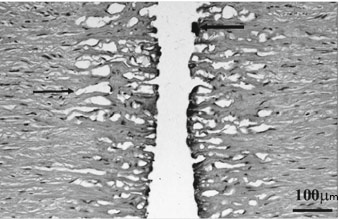
\includegraphics[width=\columnwidth]{./ablation/images/steam_vacoule.png}
	\caption{Tissue ablations, as viewed under a microscope. Steam vacuoles are clearly visible either side of the ablation area. Carbonisation is also evident at the edges of the ablation fronts. Adapted from~\cite{welch2011optical}.}
	\label{fig:histology}
	\vspace{-10pt}
\end{figure}

\subsubsection{Modelling coagulation damage}

With the description of the various process that tissue undergoes during ablation, we can now create a numerical model of these processes.
First, in order to model the full extent of the damage done under 100${^{\circ}}$C, i.e in the coagulation regime, we use the Arrhenius damage model. The Arrhenius damage model was originally used as a kinetic model of reaction products in chemistry~\cite{pearce2009relationship}. It has since been adapted by various authors for modelling tissue damage \cite{hendriques1947studies,jiang2002effects}. These authors and various others, adapted this model by fitting \cref{eqn:arrhenius} to experimental data for burn damage. The two paramters fitted in this way are the A, the frequency factor, and $\Delta E$, the activation energy.

\begin{equation}
\Omega(t)=\int^{t_{f}}_{t_i} Ae^{(-\tfrac{\Delta E}{RT})}d\tau
\label{eqn:arrhenius}
\end{equation}


\noindent Where:

	\indent $\Omega$ is the damage value;
	
	\indent A is `frequency factor' [$s^{-1}$];
	
	\indent $\Delta E$ is activation energy [$J\cdot mol^{-1}$];
	
	\indent R is the universal gas constant [$J\cdot mol^{-1}\cdot K^{-1}$];
	
	\indent T is the temperature [$K$];
	
	\indent and $t_i$ and $t_f$ are the initial time and final time at $t_{crit}$.
	
	\medskip

It is reported that a value of $\Omega$ of 0.53, 1.0, and 10$^4$ relate to first, second, and third degree burns respectively~\cite{diller1983finite}. We use the Arrhenius damage model in order to better understand the amount of damage caused by the laser in the non-ablated areas of tissue. This can give us an insight into the various physical phenomena encountered in the \gls{oct} results.

\subsubsection{Modelling physical tissue damage}

As tissue is generally mostly consists of water *ref* when the temperature of the tissue approaches 100$^{\circ}$C (at 1 atm), water in the tissue begins to boil off. This acts as a large heat sink for the absorbed laser energy, slowing down the rate of ablation. The energy required to boil the water is $Q_{vapor}=m_v\cdot L$, where $m_v$ is the mass of a voxel, and $L$ is the latent heat of vaporisation. The energy to boil off the water is provided via the laser and heat diffusing into the voxel:

\begin{equation}
Q_{vapor}=\underbrace{laserOn\cdot\dot{q}\cdot \Delta t\cdot V_{i,j,k}}_\text{laser heating} + \underbrace{c\cdot M_{i,j,k}\cdot\Delta T}_\text{heat diffusion}
\end{equation}

\noindent Where:

	\indent $Q_{vapor}$ is the current energy in Joules that has been used to boil off the water in the voxel [$J$];
	
	\indent $laserOn$ is a boolean variable that determine if the laser is on or off [$-$];
	
	\indent $\dot{q}$ is the energy absorbed by the voxel due to the laser [$W\cdot m^{-3}$];
	
	\indent $\Delta t$ is the timestep [$s$];
	
	\indent $V_{i,j,k}$ is the volume of the $i^{th}$, $j^{th}$, $k^{th}$ voxel [$m^3$];
	
	\indent $c$ is the heat capacity of the voxel [$J\cdot K^{-1}$];
	
	\indent $M_{i,j,k}$ is the mass of the $i^{th}$, $j^{th}$, $k^{th}$ voxel [$Kg$];
	
	\indent and $\Delta T$ is the change in temperature the voxel would undergo, if the water was not boiling off.

	\medskip
	
As water boils off, the water content of each voxel changes. This affects the absorption coefficient, density, thermal conductivity, and heat capacity. Each of these vary linearly with water content per voxel\cite{choi2001analysis};

\begin{align}
W &= W_{init} - \left(W_{init} \cdot \left(\tfrac{Q_{current}}{Q_{vaporisation}}\right)\right) \\
\rho &= \frac{1000}{W + 0.649\cdot P} \\
c_p &= 4.2\cdot 10^{3}\cdot W + 1.09\cdot 10^{3}\cdot P \\
\kappa &= \rho \cdot (6.28\cdot 10^{-4}\cdot W + 1.17\cdot 10^{-4} \cdot P)\\
\mu_a &= W \cdot \mu_{water} + \mu_{protein}\\
\end{align}

\noindent Where:

\indent $W$ is the water content (i.e W = 0.7 equates to 70\% water content);

\indent $W_{init}$ is the initial water content;

\indent $Q_{current}$ is the total energy absorbed by the $i^{th}$ voxel since the temperature reached 100$^{\circ}$C [$J$];

\indent $P$ is the protein content (i.e P = 1.0 - W);

\indent $\kappa$ is the Thermal conductivity [$W\cdot m^{-1}\cdot K^{-1}$];

\indent $c_p$ is the heat capacity [$J\cdot Kg^{-1}\cdot K^{-1}$];

\indent and $\mu_a$ is the total absorption coefficient, and $\mu_{water}\ \text{and}\ \mu_{protein}$ are the absorption coefficients of water and protein respectively.

\medskip

We define the \gls{ta} as occurring between 177 and 500$^{\circ}$C\cite{gerstmann1994char,mckenzie1986three}. At \gls{ta} the tissue is removed and the thermal, optical, and physical properties set to that of air.

The tissue structure is then fed back to the \gls{mcrt} model and the whole process repeats until the predefined time limit is reached. This process is outlined in \cref{fig:algo}.

\section{\textit{In silco} results} 

\subsection{Introduction}%************************************************************************************************************************************************************************

In order to match the experimental results, we must first create as accurate model of the experimental setup \textit{in silico}. However due to computational constraints, such as memory and time available, we must make some approximations to the experimental setup. The porcine skin was a large thin slice of the top most layers of the skin. However as the area of interest is where the ablation occurs, we initially  model the porcine skin as a cuboid, dimensions:  1.1 $\times$ 1.1 $\times$ 0.5 cm. The initial temperature of the porcine skin is assumed to be around 5$^{\circ}$, as the tissue was kept on ice or was kept cooled. 
As mentioned in the previous sections, there are several unknowns in the model: \gls{ta}, water content, temperature of air after ablation, and the exact thermal and optical properties of the porcine tissue. Therefore we run several models so that the full parameter space of these unknowns can be explored.
Results from these \textit{in silico} experiments are presented in this section along with a comparison of the model to the experimental work carried out in collaboration with the University of Dundee and the photobiology department at Ninewells hospital.


\subsubsection{Optical \& thermal properties}

As mentioned, the thermal and optical properties of porcine tissue are not known exactly for a given tissue sample. This is due to no one tissue sample being exactly the same as another sample, due to various factors. As such the thermal and optical properties used in this section are taken from various literature source and are modified over a range that is deemed acceptable according to various sources.

Both of the lasers used in the experimental work are infrared lasers, this means that the optical properties of the tissue are dominated by water absorption (see \cref{fig:waterabsor}). The lasers used in the experiment are the Lynton lumina 576 Er:YAG, and the Pixel CO$_2$. The Er:YAG laser has a wavelength 2940$~nm$ which corresponds to an absorption coefficient of water: $\sim 11200~cm^{-1}$. The CO$_2$ laser has a wavelength 10.6$~\mu m$ which corresponds to an absorption of coefficient of $\sim 850~cm^{-1}$. As the absorption coefficient is large, we assume that scattering is negligent at these wavelengths.
\Cref{table:values} summarises the thermal properties for tissue and air used in the simulations.  

\begin{figure}	
\vspace{-10pt}
	\centering
	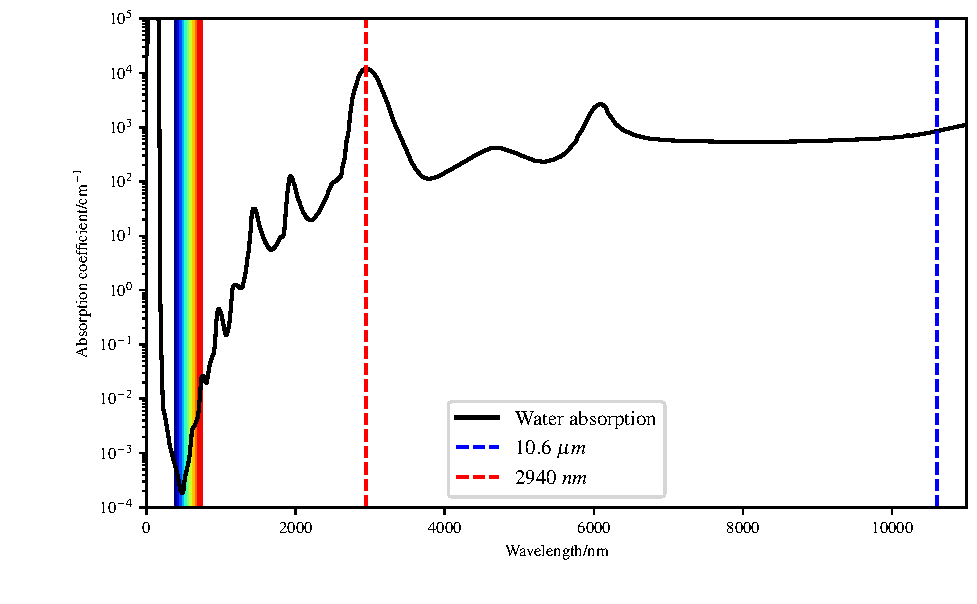
\includegraphics[width=\columnwidth]{./ablation/images/water.pdf}
	\caption{Water absorption coefficient for wavelengths 0-12000nm \cite{segelstein1981complex}. Data shows that water is highly absorbing in the infra-red portion of the spectrum.}
	\label{fig:waterabsor}
	\vspace{-10pt}
\end{figure}

\begin{table}
\begin{tabular}{|c|c|c|c|}
\hline 
• & Thermal conductivity, $\kappa$  & Density, $\rho$ & Heat capacity, c \\ 
\hline 
Tissue & $\rho \cdot (6.28\cdot 10^{-4}\cdot W + 1.17\cdot 10^{-4} \cdot P)$ & $\frac{1000}{W + 0.649\cdot P}$ & $4.2\cdot 10^{3}\cdot W + 1.09\cdot 10^{3}\cdot P$  \\ 
\hline 
Air & $a e^{-b(T-273.15)} +c$  & $\tfrac{p_{atm}}{R_{spec} T}$ & 1006 \\ 
\hline 
\end{tabular}
\caption{blah blah}\label{table:values}
\end{table}  

Both lasers were used in `Pixel beam' mode. This means that the laser beam is split into an array of smaller beams. The Er:YAG laser used a pattern of 5 x 5 lasers, with the corners missing, giving a total of 21 `Pixel beams'. The CO$_2$ laser used an array of 81 pixel beams with no missing `Pixels'. As the CO$_2$ laser was upgraded during the period in which the experimental data was taken, we present both sets of data, pre-upgrade and post-upgrade. The upgrade consisted of an update to the laser power, from 30~$W$ to 70~$W$.

Both lasers operated in different modes; the Er:YAG delivered multiples pulses of either 350~$mJ$ or 700~$mJ$, and the CO$_2$ delivered one single pulse of varying energy over the range 50~$mJ$ to 400~$mJ$. The experiment consisted of ablating the porcine tissue, as a function of energy per `pixel' beam. This was achieved by either stacking multiple pulses on top of each other for the Er:YAG laser over a range of 350~$mJ$ to 3500~$mJ$. For the CO$_2$ the pulse length of each pulse was adjusted, so that the energy per pulse was varied over a range 50~$mJ$ to 400~$mJ$. The energy range for the CO$_2$ laser was kept the same pre and post-upgrade.

\subsubsection{Computational speed up:}
As mentioned in the introduction, the volume of interest is the are around the ablation craters. The volume is 1.1 $\times$ 1.1 $\times$ 0.5~$cm$. However, in order for the simulation to have good resolution of the ablation craters, this volume would require a large number of voxels for the tissue model. This is unfeasible due to: the memory required to store the various counters, and variables, and the time that would be required in order to carry out the computation. Thus the volume of interest is reduced to focus on just one of the ablation craters that is created by the laser.
As a sanity check to ensure that we are not omitting any phenomena by focusing on just one ablation crater, an initial simulation that simulates the full volume of interest was carried out to investigate the possibility of overlapping craters or other related phenomena. The simulation, as shown in~\cref{fig:sizecheck}, gives us validation that the shrinking of the volume of interest is a valid approximation to make.

\begin{figure}
	\centering
    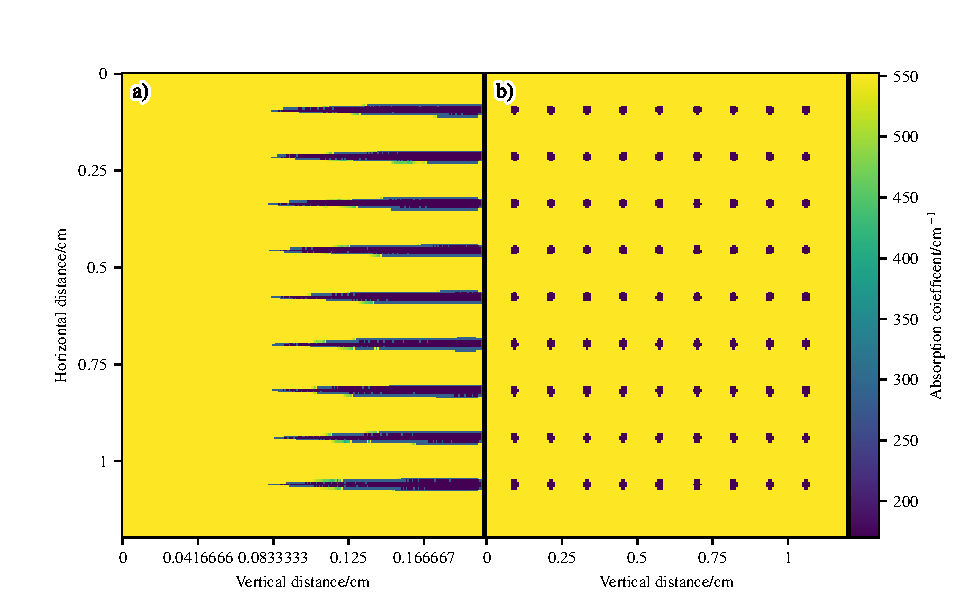
\includegraphics[width=\columnwidth]{./ablation/images/slice.pdf}
    \caption{Simulation of 81 pixel beams. Figure is a slice through the optical properties at the end of the simulation. Yellow is unchanged tissue, and purple is completly ablated tissue.}\label{fig:sizecheck}
\end{figure}

\subsection{Results}

\subsubsection{Investigating ablation temperature, \texorpdfstring{$T_a$}{Ta}}

Various literature sources report the ablation temperature ranging from 177$^{\circ}$ to 500$^{\circ}$~\cite{gerstmann1994char,mckenzie1986three}. Thus, we run several models over this range in order to establish a `good' \gls{ta} to use for the rest of the simulations. \Cref{fig:ta} shows how \gls{ta} affects the crater depth as a function of pixel beam energy for the CO$_2$ laser. Both the 70~$W$ and 30~$W$ simulations agree, that a `good' \gls{ta} is around $T_a=400~^{\circ}C$.

Increasing the ablation temperature, has the obvious affect of requiring more energy to be deposited by the laser before ablation takes place. As more energy is required to heat the porcine tissue up to the ablation temperature before it can be ablated. Decreasing the ablation temperature has the converse affect.

Over the full range of \gls{ta}, as the energy per pixel beam increases, there is a trend that at higher energies the crater depth tapers off.  


\begin{figure}
	\centering
    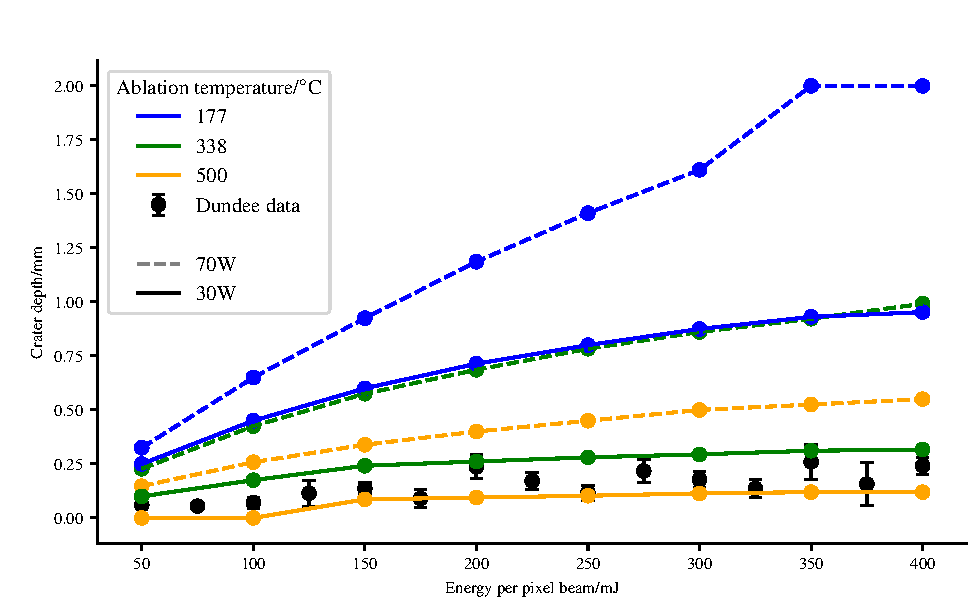
\includegraphics[width=\columnwidth]{./ablation/images/both.pdf}
    \caption{Simulations of 30~$W$ and 70~$W$ CO$_2$ ablative laser. Crater depths as a function of pixel beam energy for various \gls{ta}'s. *placeholder until I get 70W dundee data. need to rerun the upper 177 points on larger z depth as it crashes currently*}\label{fig:ta}
\end{figure}
 

\subsubsection{Investigating Thermal damage} 
 
\subsubsection{Comparison to experimental work} 
 
*The work below will possibly be done. If so it will be in 2019 if not needed for the paper*
\subsubsection{Effect of thermal and optical properties on crater depth}

As mentioned in the introduction to this section, the thermal and optical properties vary over a wide range in the literature. Thus there is no one `correct' value we can choose for out simulations. In order to better understand how the thermal and optical properties affect the crater depth reached by the fractional laser, we vary the properties by $20\%$. This section presents the results of changing the thermal optical properties: heat capacity, thermal conductivity, protein and water absorption, and density.

\paragraph{Heat capacity, $c_p$}
\paragraph{Thermal conductivity, $\kappa$}
\paragraph{Absorption coefficient, $\mu_a$}
\paragraph{Density, $\rho$}


\subsubsection{Investigating water content}
 
\subsubsection{Investigating temperature of air after ablation}  
*****************************************************************
\section{Conclusion}
\chapter{Quasi-wave/particle Monte Carlo Algorithm, \texorpdfstring{$\varphi MC$}{phiMC}}\label{sec:phase}

\section{Introduction}\label{sec:besintro}

Complex shaped light beams have been used in a wide variety of applications in biophotonics and medicine.
From using Airy beams to move particles and cells~\cite{baumgartl2008optically}, Bessel beam ``tractor beams''~\cite{ruffner2012optical}, Airy and Bessel beams for better field of view in light-sheet microscopy~\cite{vettenburg2014light}, and utilising Laguerre-Gaussian beams to optical trap optically reflective particles~\cite{simpson1996optical}.


However, simulation techniques for modelling complex shaped beams in biological tissue is lacking.
Currently there are several techniques that can model these beams in biological tissue, however they all have downsides.
These methods include diffusion approximation to the~\gls*{rte}, \gls*{fdtd}, \gls*{pstd}, \gls*{bpms}, and \gls*{mcrt}.

As discussed in~\nameref{sec:diffusionapprox}, the diffusion approximation has many issues when it comes to modelling light propagation in biological tissue.
\gls*{fdtd} involves using a finite difference method to solve Maxwell's equations.
This is computationally intensive and requires a grid resolution of $\sim \lambda/20$ and thus most models are restricted to 2D~\cite{glaser2016fractal,elmaklizi2015penetration}. 
\gls*{pstd} like the \gls*{fdtd} is also computationally intensive, though to a lesser extent~\cite{glaser2016fractal}.
\Gls*{bpm} is a fairly computational efficient method of propagating light beams, compared to~\gls*{fdtd} or~\gls*{pstd}.
However, the~\gls*{bpm} uses the slowly varying envelope approximation, which limits some of the problems it can be applied.
\Gls*{bpm} is also generally a uni-directional propagation method, though it can be adapted to model bidirectional propagation, this can lead to issues in the model's accuracy~\cite{van1981beam,glaser2016fractal}.

\medskip

The final method,~\gls*{mcrt}, in general, cannot model complex beams where the wave-like behaviour of photons is required to form, or propagate the beam.
For example, traditional \gls*{mcrt} methods cannot model Gaussian beams, as Gaussian beams have a finite beam waist at their focus (see~\cref{fig:gbeamills}).
\Gls*{mcrt} (along with geometric optics) predicts that Gaussian beams have an infinitely small waist.

Various authors have tried to model complex beams that require wavelike behaviours using~\gls*{mcrt}.
Some of the techniques used by these authors include: artificial beam steering~\cite{hokr2015modeling}, generating skew rays~\cite{arnaud1985representation}, complex ray tracing~\cite{harvey2015modeling}, decomposition~\cite{worku2018decomposition}, electric field Monte Carlo~\cite{cai2014electric}, and wavefront tracing~\cite{volpe2017huygens}.
However, all these techniques either inaccurately model Gaussian beams, can model Gaussian beams but are complex to implement or computational intensive (more so than \gls*{mcrt} usually is).
There have been some attempts at using the techniques presented in this chapter, to modify MCRT algorithms into algorithms that can model diffraction and interference~\cite{mignon2016fractional,peter2014combining,mahan2018monte,mout2016simulating,fischer2008monte}.
These authors have good results, but either do not detail their methods, do not attempt to treat scattering or are in the x-ray regime.


This chapter modifies the MCRT method, from a ``ballistic'' photon method into a quasi-ballistic/wave photon method so that the wave behaviour of photons can be modelled.
This algorithm, $\varphi MC$, allows the modelling of complex shaped beams such as Bessel beams and Gaussian beams, without much modification of the underlying \gls*{mcrt} code.

We present a thorough investigation of the method used to turn a ballistic regime~\gls*{mcrt} method in to a quasi-wave/ballistic method.
The method is validated against theoretical and experimental data for various different beam types including: Bessel (including higher orders), and Gaussian beams.
Treatment of the propagation through scattering media is also discussed.


\section{Theory}\label{sec:bestheory}

To convert a MCRT simulation to be able to model wave-like behaviour of photons, we introduce two concepts: tracking the complex phase of packets and the Huygens-Fresnel principle.
This section presents a description of the modifications to the traditional MCRT algorithm, alongside the theoretical background to both the concepts.

\subsection{Complex Phase Tracking}

The first concept we add to the MCRT method is assigning a complex phase to each packet.
The phase is given to a packet at the beginning of the simulation depending on the input field.
The packet is also given an initial electric field of the form:

\begin{equation}
E_0 = \frac{1}{N}\sqrt{\frac{P}{A}}
\label{eqn:initefield}
\end{equation}

Where $N$ is the number of packets run in a simulation, $P$ is the power of the incident beam, and $A$ is the area of the beam.
This initial electric field is needed to compare different beams as in~\cref{sec:compBeams}, and to normalise for number of packets run.

The phase is then tracked as the packet moves through the medium, over a distance $l$.
~\Cref{eqn:phase} shows how the phase is calculated.

\begin{equation}
    \varphi = cos\left(\frac{2 \pi l}{\lambda}\right) + i\ sin\left(\frac{2 \pi l}{\lambda}\right)
    \label{eqn:phase}
\end{equation}

Where $\varphi$ is the complex phase of a photon packet, $l\ [m]$ is the distance the packet has travelled, $\lambda~[m]$ is the wavelength of the packet.
Now we can calculate the complex phase of a packet at a position $P_o$, if we know the distance it has travelled, and its original phase, see~\cref{fig:phase-diag}.

\begin{figure}[!htbp]
    \centering
    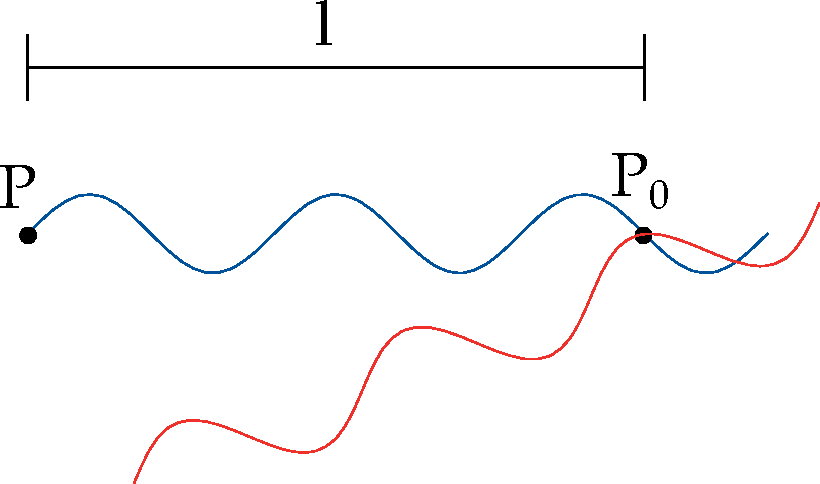
\includegraphics[width=0.5\textwidth]{phase-diag.pdf}
    \caption{Example of phase calculation when a photon has travelled a distance l. The figure also shows an example of interference between two photons via addition of the complex amplitudes at the point $P_0$.}
    \label{fig:phase-diag}
\end{figure}

To model interference, we let the photon packets interfere with one another in a volume or area element. 
We do not model the interference at a point in space where photon packets cross, due to the ballistic nature of the \gls*{mcrt} simulation this does not occur with enough frequency to give a good signal to noise ratio. 
Therefore, interference takes place in a volume, $dV$, or area element, $dA$, instead.
To calculate the intensity from the complex phase, the absolute value of the phase is squared.
Therefore to calculate the intensity for a given voxel or area, the phase is first summed in each voxel or area before the absolute value is squared.~\Cref{eqn:intense} shows the equation for intensity for a volume element $dV$. A similar relation for calculating the interference on an area element $dA$ also exists.

\begin{equation}
I(\zeta)= \left| \sum\limits_{\zeta}E_0\ cos\left(\frac{2\pi l}{\lambda}\right) + i \sum\limits_{\zeta}E_0\ sin\left(\frac{2\pi l}{\lambda}\right)\right|^2,\ \ \ \zeta=(x,y,z)
\label{eqn:intense}
\end{equation}

\noindent Where:

\indent $l$ is the total distance travelled by a photon [$m$];

\indent $\lambda$ is the wavelength of the photon [$m$];

\indent $I$ is the intensity at the $\zeta^{th}$ cell [$W m^{-2}$];

\indent $E_0$ is the initial electric field of the packets as in~\cref{eqn:initefield} [$Vm^{-1}$]

\indent and $\zeta$ is the $x^{th}$, $y^{th}$, $z^{th}$ cell, volume $dV$.

\medskip

In addition to tracking the phase, the next principle needed to simulate the wave behaviour of light in MCRT is the Huygens-Fresnel principle.

\subsection{Huygens-Fresnel Principle}

The Huygens-Fresnel principle is a method that is used to help model the propagation of waves in the far field limit and the near field limit. 
The Huygens principle was first postulated in 1678 and states~\cite{huygens2012treatise,hecht2017optics,huygens1900wave}: 

\medskip

``\textit{Every point on a propagating wavefront serves as the source of spherical secondary wavelets, such as the source at some time later is the envelope of these wavelets.}''

\medskip

The principle is illustrated in~\cref{fig:huygensillis}.
The principle allowed Huygens to derive laws of refraction and reflection, but it failed to describe diffraction effects.
This led to Augustin-Jean Fresnel in 1818, combining the Huygens principle with his own theory of interference~\cite{fresnel1819memoire,huygens1900wave}.
This Huygens-Fresnel principle, gave an accurate description of the propagation of light and diffraction effects.
This was achieved by allowing the secondary wavelets to self interfere, giving rise to an accurate description of the physical phenomena.
Later, Gustav Kirchhoff gave a rigours mathematical description of the Huygens-Fresnel principle, which is the basis of diffraction theory~\cite{kirchhoff1883ann,born2000principles}. 

The Huygens-Fresnel principle allows the modelling of diffraction in both the near and far field.
As the principle states that every point on the wavefront is a source of secondary spherical waves, this implies that there are ``backward'' waves.
These ``backward'' waves are un-physical, and there is no experimental evidence of their existence.
Thus, Fresnel introduced an inclination factor to eliminate these ``backward'' waves.
This inclination factor was later put on a rigorous mathematical standing by Kirchoff, as it naturally fell out of his theory~\cite{kirchhoff1883ann,born2000principles}.
\Cref{eqn:kirchhoffeqn}, the Rayleigh-Sommerfeld diffraction integral of the first kind\footnote{If diffraction occurs in a plane, the Kirchoff diffraction integral can be modified to this}, shows the equation for the complex field at a point on a plane.

\begin{equation}
u(\mathbf{r_1})=\frac{1}{i\lambda}\int\int u(\mathbf{r_0})\frac{\mathbf{\hat{s_0}} \cdot (\mathbf{r_1} - \mathbf{r_0})}{\left|\mathbf{r_1} - \mathbf{r_0}\right|^2}e^{ik\left|\mathbf{r_1} - \mathbf{r_0}\right|}dS_0
\label{eqn:kirchhoffeqn}
\end{equation}

\noindent Where:

    \indent $u$ is the complex electric field [$Vm^{-1}$];

    \indent $\lambda$ is the wavelength [$m$];

    \indent $S_0$ is a plane with surface normal $\mathbf{\hat{s_0}}$ [-];

    \indent $k$ is the wavenumber [$m^{-1}$];

    \indent and $\mathbf{r_n}$ are spatial coordinates [-]. 

\medskip

The Huygens-Fresnel principle is implemented by sampling the light source on the surface of any lens or in a slit.
In practise this means when for example, a plane wave is incident on a slit width \textit{a}, and length \textit{b}, the slit area is uniformly sampled for the initial position of the photon packets.
The packets are then given a random direction, sampled towards the detector thus avoiding the non-existent ``backward'' waves.
For the case of modelling propagation through a lens, the usual geometric optics approach is taken to propagate the packets through the lens.
When the packet lies on the surface of the lens, the Huygens-Fresnel principle is invoked, and the packet is given a random direction (in the direction of the medium) and propagated as usual.

\medskip

Our algorithm uses the Huygens-Fresnel principle and the tracking of complex phase to simulate diffraction effects, that would otherwise be absent from the simulation.
The principle allows the algorithm to calculate the complex amplitude at a point, and thus the intensity at that point, essentially numerically simulating~\cref{eqn:kirchhoffeqn}.
These two concepts underpin the algorithm that allows various complex beams, and wave phenomena to be simulated within a ballistic method. The following sections validate the method against the theory and experimental data for propagation of various complex beams.

\begin{figure}[!htbp]
    \centering
    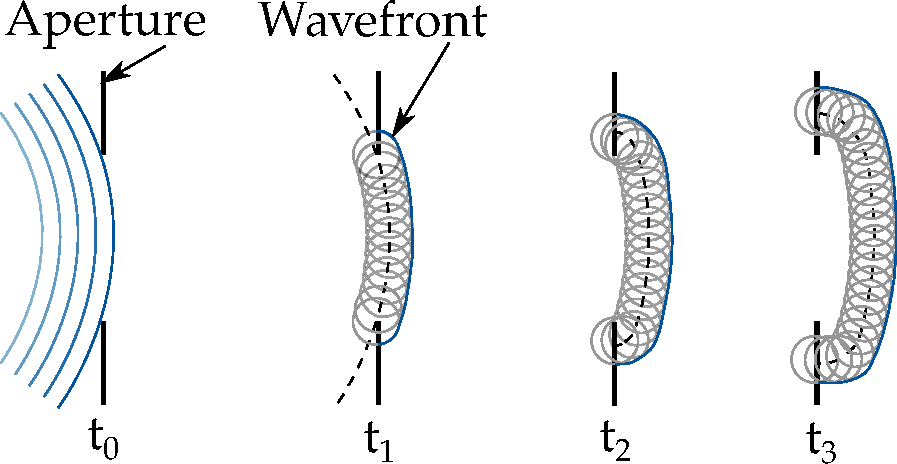
\includegraphics[width=0.7\textwidth]{huygens.pdf}
    \caption{Illustration of the Huygens-Fresnel principle. At $t_0$ a wave is incident on an aperture. Times $t_1,\ t_2,\ \text{and}\ t_3$ show the evolution of the wavefront using the Huygens-Fresnel principle. Dashed lines illustrate the wavefront position at the previous time step, and is the source of the Huygens-Fresnel wavelets.}
    \label{fig:huygensillis}
\end{figure}

\subsection{Validation of Phase Tracking Algorithm}

\subsubsection*{Double Slit Experiment}

The first test of our quasi-wave/particle MCRT algorithm\footnote{Though this example is not strictly MCRT, but rather ray tracing, as it involves no scattering. The full MCRT method will be used in later sections.}, $\varphi MC$, is to compare our simulation to a double slit experiment.
The double slit experiment, is a simple experiment where a monochromatic plane wave of light is incident on two slits distance apart $d$, and width $b$, and an interference pattern is observed on a screen a distance $L$ away from the slits. The experiment is usually carried out with the detector screen in the far field (the so called Fraunhofer regime).
The intensity pattern on the detector screen is as in~\cref{eqn:doubleslit}:

\begin{equation}
    I(x) \propto cos^2\left(\frac{kdx}{2\sqrt{L^2+x^2}}\right)sinc^2\left(\frac{kax}{\sqrt{L^2+x^2}}\right)
    \label{eqn:doubleslit}
\end{equation}

Where the $sinc$ function is defined as $\tfrac{sin(x)}{x}$, for $x\ \neq 0$, $k$ is the wavevector, $k=\tfrac{2\pi}{\lambda}$, and $x$ is the horizontal position on the detector screen.

The simulation was carried out for a wavelength, $\lambda$,  of $488~nm$, a slit width of $10\lambda$, slit separation of $80\lambda$, and the detector screen positioned $10000\lambda$ away from the slits.
Using the Huygens-Fresnel principle, each slit is a source of Huygens wavelets.
The detector screen has dimensions, $1~mm^2$ and there are $2051^2$ bins, giving a bin an effective size: $\sim 488~nm$ or $\sim \lambda$.
The initial position of the photon packets is sampled uniformly from the slit area, after randomly choosing one of the slits to emit from.
A random direction is then chosen to ensure that the packets will hit the detector screen.
The simulation was run with $10^9$ packets, which took $\approx10~mins$ to run on an 8 core Intel Xeon machine.
This gave an accurate match to the theoretical expression, as seen in~\cref{fig:doubleslitcomp}.

\begin{figure}[!htbp]
    \centering
    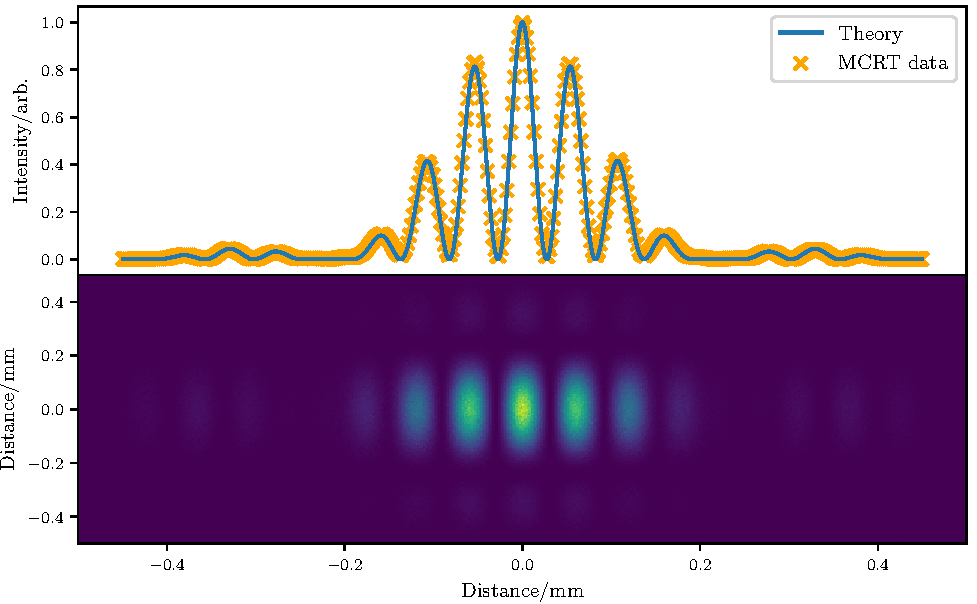
\includegraphics[width=0.75\textwidth]{doubleslit.pdf}
    \caption{Comparison of theory and simulation for the double slit experiment. Top image shows a slice through the computed image and the expected profile from theory. For clarity only every $5^{th}$ MCRT data point is plotted. Bottom image shows the computed image.}
    \label{fig:doubleslitcomp}
\end{figure}

\subsubsection*{Diffraction by a Square Slit}
$\varphi MC$ is also validated by simulating diffraction from a square aperture in the far and near field. 
Fresnel diffraction occurs in the near field when the \textit{Fresnel number},~\cref{eqn:fnumber}, is greater than 1.0.
Fraunhofer diffraction occurs when the \textit{Fresnel number} is less than 1.0.

\begin{equation}
F = l\sqrt{\frac{2}{\lambda r_0}}
\label{eqn:fnumber}
\end{equation}

\Cref{eqn:fnumber} is the Fresnel number, where \textit{l} is the slit width, $\lambda$ is the wavelength of the incident radiation, and $r_0$ is the distance from the aperture to the detector screen, as shown in~\cref{fig:aperture}. 

\medskip
\begin{figure}[!htbp]
    \centering
    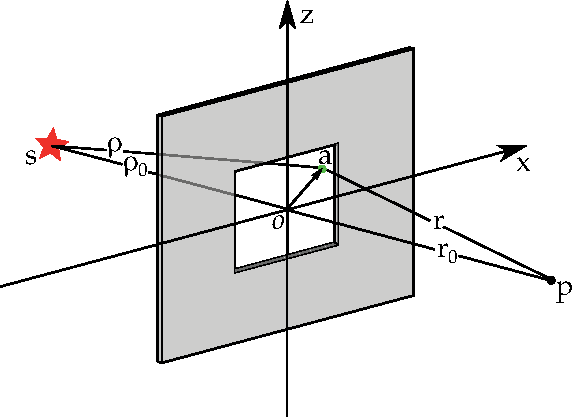
\includegraphics[width=0.75\textwidth]{aperture.pdf}
    \caption{Geometry of the square aperture used in the validation.}
    \label{fig:aperture}
\end{figure}

To compare $\varphi MC$ to the theory, the theory must first be discussed.
Consider the setup as shown in~\cref{fig:aperture}, to calculate the intensity at a point $P$ the contribution by an area element $dS$ at the point $a$, to the optical disturbance at a point \textit{P} is considered.
Accounting for the unobstructed optical disturbance from $S$ as well and using~\cref{eqn:kirchhoffeqn}, yields: 


\begin{equation}
U(P)=\frac{1}{i\lambda}\iint\limits_{\Sigma} \frac{Ae^{i(k\rho-\omega t)}}{\rho} \frac{e^{ikr}}{r}cos(\theta)\ dS
\label{eqn:disturb}
\end{equation}


In the case where $\rho_0$ and $r_0$ are large compared to the size of the aperture, then $\cos\left(\theta\right) = 1$ and $\tfrac{1}{\rho r}=\tfrac{1}{\rho_0 r_0}$.
The lengths of $r_0$ and $\rho_0$ are:

\begin{align}
r=&\sqrt{r_0^2+y^2+z^2}\label{eqn:r} \\
\rho=&\sqrt{\rho_0^2+y^2+z^2}\label{eqn:rho}
\end{align}

Using the binomial theorem to expand~\cref{eqn:r,eqn:rho} yields:

\begin{equation}
\rho + r \approx \rho_0 + r_0 + (y^2+z^2)\frac{\rho_0r_0}{2\rho_0r_0}
\label{eqn:binomial}
\end{equation}

Substituting~\cref{eqn:binomial} into~\cref{eqn:disturb} with $k=2\pi/\lambda$

\begin{equation}
U(P)=\frac{Ae^{-i[k(\rho_0+r_0)\omega t]}}{i\lambda\rho_0r_0}\iint\limits_{\Sigma} e^{i2\pi y^2\tfrac{(\rho_0+r_0)}{2\lambda\rho_0r_0}+i2\pi z^2e^{\frac{i\pi u^2}{2}}\tfrac{(\rho_0+r_0)}{2\lambda\rho_0r_0}} \ dS
\label{eqn:midway}
\end{equation}


Introducing the dimensionless variables \textit{u} and \textit{v}

\begin{align}
u&=y\sqrt{\frac{2(\rho_0+r_0)}{\lambda\rho_0r_0}}\\
v&=z\sqrt{\frac{2(\rho_0+r_0)}{\lambda\rho_0r_0}}
\end{align}

and substituting them into~\cref{eqn:midway}.

\begin{equation}
U(P)=\frac{\tilde{E}_u}{2}\int_{u_1}^{u_2} e^{\tfrac{i\pi u^2}{2}}\ du\int_{v_1}^{v_2} e^{\tfrac{i\pi v^2}{2}} \ dv
\label{eqn:pentdisturb}
\end{equation}
\Cref{eqn:pentdisturb} describes the optical disturbance at the point $P$, with $\tilde{E}_u$ the unobstructed disturbance at $P$.
\Cref{eqn:pentdisturb} can be evaluated using the Fresnel integrals, $C(w)$ and $S(w)$:


\begin{equation}
\int_{0}^{w}e^{i\pi w'^2/2}dw'=C(w)+iS(w)
\label{eqn:fresneleqn}
\end{equation}


\begin{align}
S(w)&=\int^w_0 sin\left(\frac{\pi w'^2}{2}\right)dw'\label{eqn:fresint1}\\
C(w)&=\int^w_0 cos\left(\frac{\pi w'^2}{2}\right)dw'\label{eqn:fresint2}
\end{align}


Using~\cref{eqn:fresneleqn}, where $C(w)$ and $S(w)$ are the Fresnel integrals as in~\cref{eqn:fresint1,eqn:fresint2}.
\Cref{eqn:pentdisturb} can then be transformed into an intensity, by taking the absolute value and squaring, yielding~\cref{eqn:fresIntensityp}:


\begin{equation}
I_p = \frac{I_u}{4} \{[C(u_2) - C(u1)]^2 + [S(u_2) - S(u_1)]^2\} \times \{[C(v_2) - C(v_1)]^2 + [S(v_2) - S(v_1)]^2\}
\label{eqn:fresIntensityp}
\end{equation}

\Cref{eqn:fresIntensityp} gives the intensity of the field at the point $P$ on axis for a square aperture where $I_u$ is the unobstructed intensity at the point $P$. 

\medskip

As the mathematics of calculating the optical disturbances at all points on a plane at point $P$ is difficult, instead the aperture is moved by small displacements, with $\overrightarrow{SOP}$ fixed.
This effectively achieves the translation of the origin, $O$, with respect to the fixed aperture. 
Thus, for each displacement new aperture coordinates $y_1$, $y_2$, $z_1$, and $z_2$ are generated and therefore new $u_1$, $u_2$, $v_1$, and $v_2$.
Therefore the intensity at a point $P +\delta d$, where $\delta d$ is the displacement, can be calculated.
This approximation holds for displacements that are small compared to the $\rho_0$~\cite{born2000principles,hecht2017optics,goodman2017introduction}.
Using this method and~\cref{eqn:fresIntensityp} gives the theoretical curves in~\cref{fig:frescompare}.

\medskip

In $\varphi MC$, the above experiment is simulated. 
A square slit is uniformly sampled in the $x$, and $z$ direction to get the packets initial position. 
A random direction is then sampled, by uniformly picking a point on the detector screen.
This ensures the algorithm does not waste time by calculating packets trajectories that are not registered by the detector.
We assume a plane wave is incident on the aperture and each photon is given the same initial complex electric field.

The distance between the detector screen and the aperture is varied and the intensity on the screen is measured for $\sim 10^{10}$ photons released from the aperture as Huygens wavelets.
For \textit{Fresnel numbers} greater than 1.0, the number of bins is 300, covering a distance of 600~$\mu m$. 
For the case of Fraunhofer diffraction, the number of bins is 100 covering a distance of 6000~$\mu m$.
The simulations take $\sim$ 3 minutes for $10^{10}$ packets to be run on an Intel Xeon E3--1245 v5, 8 cores @ 3.5GHz machine.
The number of bins, and photons packets simulated had to be increased for the cases where the Fresnel number was large (i.e the detector screen was near the aperture).
This is due to the diffraction pattern becoming ``noisy'' and thus needs a higher resolution to accurately simulate.
\cref{fig:frescompare} shows the comparison between the theory and the $\varphi MC$ simulations.

\begin{figure}[!htbp]
    \centering
    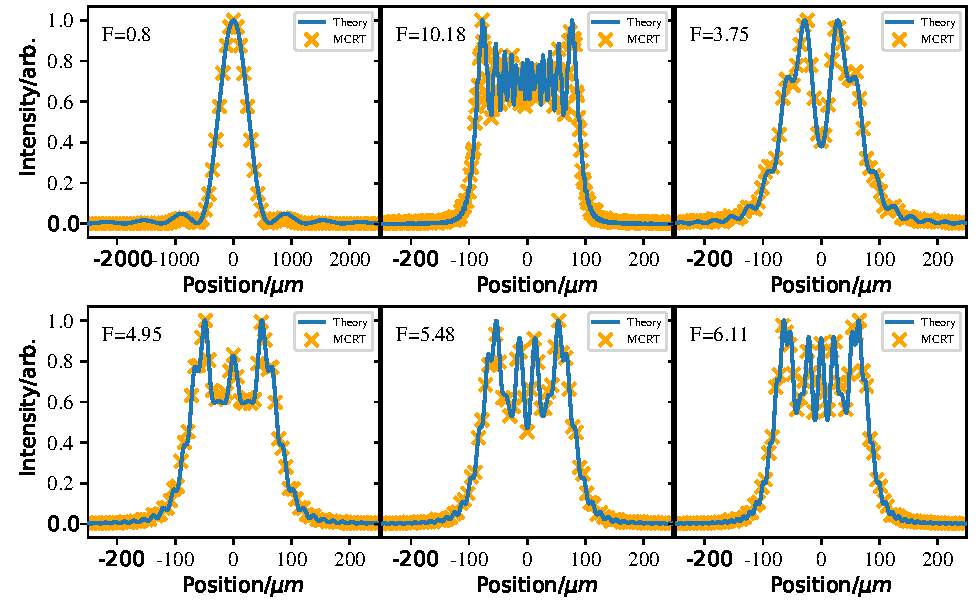
\includegraphics[width=0.95\textwidth]{Fresnel-compare.pdf}
    \caption{Comparison of theory and simulation for diffraction through a square aperture in the Fresnel and Fraunhofer regimes.}
    \label{fig:frescompare}
\end{figure}

\FloatBarrier
\newpage
\section{Gaussian Beams}

Now that the method of tracking the complex phase of packets and using the Huygens-Fresnel principle has been verified against theoretical results, we can now turn our attention to modelling the propagation of beams that require the wave behaviour of light to either form or propagate.
The first beam type we will examine is the Gaussian beam.
Gaussian beams are important as most laser beams have the profile of the fundamental (TEM$_{00}$) Gaussian mode.
This section will show that $\varphi MC$ can accurately model all the physical phenomena of Gaussian beams, within the \gls*{mcrt} regime.

Before discussing how $\varphi MC$ can model a Gaussian beam, the theory and various physical parameters of the beam must be described. 
The electric field of a Gaussian beam can be defined as in~\cref{eqn:gaussefield}~\cite{milonni2010laser}:

\begin{equation}
E(r,z)=E_0\frac{w_0}{w(z)}e^{\frac{-r^2}{w(z)^2}}e^{-i(kz+k\frac{r^2}{2R(z)}-\varphi(z))}
\label{eqn:gaussefield}
\end{equation}

\noindent Where:

    \indent $r$ is the radial distance from the optical axis [$m$];

    \indent $z$ is the axial distance from  the beams waist [$m$];

    \indent $k$ is the wavenumber, $k=\frac{2\pi}{\lambda}$ [$m^{-1}$];

    \indent $E_0$ is the electric field amplitude at the origin [$Vm^{-1}$];

    \indent $w(z)$ is the radius of the beam at which the amplitude has fallen to $\frac{1}{e}$, at the distance z along 

    \indent the beam,~\cref{eqn:gwaist} [$m$];

    \indent $w_0$ is the waist radius [$m$];

    \indent $R(z)$ is the radius of curvature of the beams wavefronts at z,~\cref{eqn:radiuscurve} [$m$];

    \indent and finally, $\varphi(z)$ is the Gouy phase at z,~\cref{eqn:gouyphase} [-].

\medskip

~\Cref{eqn:gwaist,eqn:gouyphase,eqn:rayleighrange,eqn:beamwaist,eqn:radiuscurve} give the definitions of key physical properties as outlined above or as shown in~\cref{fig:gbeamills}. 
$z_r$ is the Rayleigh range,~\cref{eqn:rayleighrange}, and defines the point at which the beams waist grows to $\sqrt{2}$ times the size of the beam at its waist.
The waist of the beam at the focal point is defined as~\cref{eqn:beamwaist}, where $f$ is the focal length and $D$ is the $\tfrac{1}{e^2}$ diameter of the beam at the lens.

\begin{align}
    w(z) &= w_0\sqrt{1+\left(\frac{z}{z_r}\right)^2} \label{eqn:gwaist} \\
    R(z) &= z\left[1+\left(\frac{z_r}{z}\right)^2\right]\label{eqn:radiuscurve}\\
    \varphi(z) &= arctan\left(\frac{z}{z_r}\right)\label{eqn:gouyphase}\\
    z_r &= \frac{\pi w_0^2}{\lambda}\label{eqn:rayleighrange}\\
    w_0 &= \frac{2\lambda f}{\pi D}\label{eqn:beamwaist}\\
\end{align}

\begin{figure}[!htbp]
    \centering
    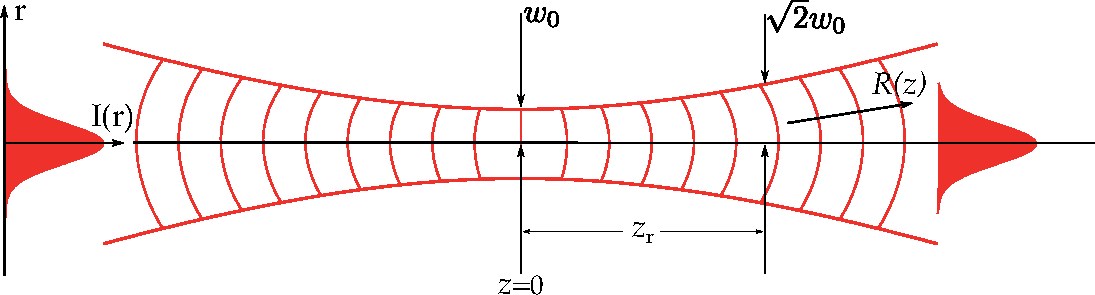
\includegraphics[width=0.95\textwidth]{gaussian-radius-curve.pdf}
    \caption{Illustration of a Gaussian beam focusing to its waist then diverging away. Image shows the various defined properties of a Gaussian beam along side the radius of curvature changing direction at the waist.}
    \label{fig:gbeamills}
\end{figure}

With the physical properties of the Gaussian beam outlined, a Gaussian beam can now be modelled using our algorithm.
To simulate a Gaussian beam, we set up the simulation as shown in~\cref{fig:gausssetup}.
The simulated lens used is a convex-plano lens, with radius of curvature, $4.6~mm$, thickness, $L_t$, of $2.2~mm$, and working distance, $W_d$, 8.5~$mm$.
A Gaussian beam wavelength $488~nm$ and $\tfrac{1}{e^2}$ waist diameter $0.5~mm$, is incident on the lens.
Using~\cref{eqn:beamwaist} yields the size of the focal spot as $3.1\mu m$.

\begin{figure}[!htbp]
    \centering
    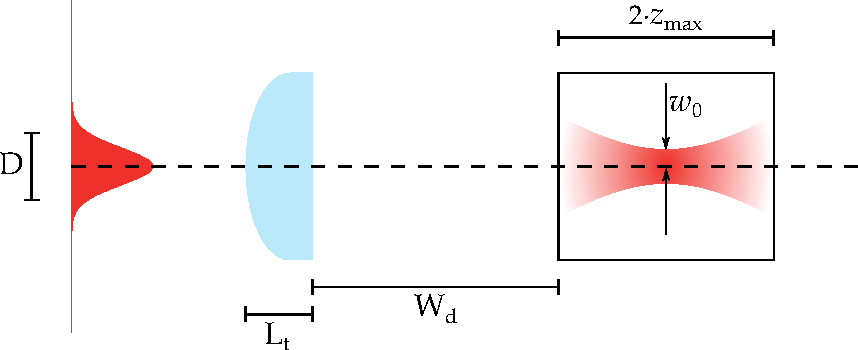
\includegraphics[width=0.75\textwidth]{gaussiansetup.pdf}
    \caption{Simulation setup of focusing a Gaussian beam through a lens. Lens is convex-plano and is modelled on ThorLabs LA4249 UV fused silica lens~\cite{thorlens}.  $L_t$ is the lens thickness, D is the $\tfrac{1}{e^2}$ input beam diameter, $W_d$ is the working distance or back focal length, $2 \cdot z_{max}$ is the depth of the medium, and $w_0$ is the beam waist.}
    \label{fig:gausssetup}
\end{figure}

To model the lens in $\varphi MC$ the photons initial z position is set just in front of the lens.
The $x$ and $y$ are randomly sampled from a Gaussian distribution with a waist of $\sqrt{2}w_0$.
The factor of $\sqrt{2}$ accounts for the conversion from intensity to electric field beam waist.
This is because the electric field is $\propto \exp{\left(\tfrac{-r^2}{4\sigma'^2}\right)}$, and the intensity is $\propto \exp{\left(\tfrac{-r^2}{2\sigma^2}\right)}$.
Thus, for the input electric field waist to be equal to the intensity,  $\sigma'=\sqrt{2}\sigma$.
The packet is given an electric field of the form~\cref{eqn:initefield}, with $P=1~mW$, and $A=\tfrac{1}{2}\pi w_0^2$.

The packet is then propagated to the surface of the convex side of the lens.
This is achieved by finding the intersection of a sphere, which represents the convex side of the lens, and the packets path.
With the packet on the surface of the lens, Fresnel coefficients are calculated to determine if the packet is reflected or refracted.
If the packet is reflected the packet is killed and the process starts again.
%***need exlanation of refraction here***
If the packet is refracted, and moved in the new direction to the planar surface of the lens.
The new direction vector is calculated using a vector version of Snell's law.
The packets are then uniformly sampled onto the surface of the voxel medium and the usual~\gls*{mcrt} method is used to propagate the packet whilst tracking the phase.

\begin{figure}[!htpb]
    \centering
    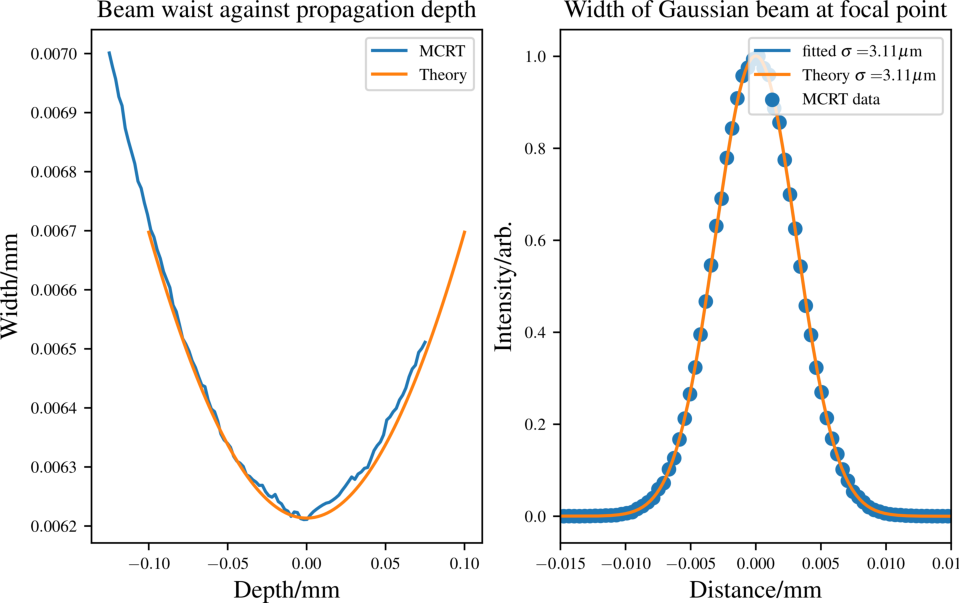
\includegraphics[width=0.75\textwidth]{gaussian.pdf}
    \caption{Results of \textit{in-silico} experiment of focusing a Gaussian beam though a convex-plano lens.}
    \label{fig:simgaussexp}
\end{figure}


\Cref{fig:simgaussexp} shows the comparison of theory and \textit{in-silico} experiment, with excellent agreement between the two.

$\varphi MC$ also correctly models the change of direction of the radius of curvature, $R(z)$, as is predicted by theory.
This process is described by~\cref{eqn:radiuscurve}, before the waist the curvature is negative, at the waist it is infinite, and past the waist its is positive.
This can be seen in~\cref{fig:proofchgrz}, where the beam (direction of propagation right to left) undergoes this:

\begin{figure}[!htpb]
    \centering
    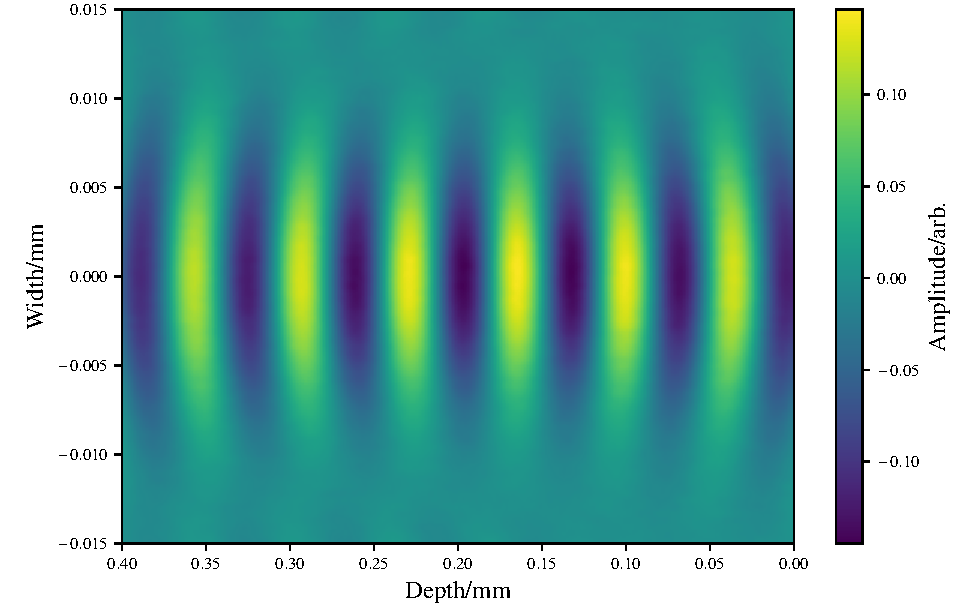
\includegraphics[width=0.75\textwidth]{radcurvechange.pdf}
    \caption{Slice through the real part of the complex electric field of the \textit{in-silico} experiment as in~\cref{fig:gausssetup}. Figure shows the radius of curvature changing direction at the waist as predicted by theory.}
    \label{fig:proofchgrz}
\end{figure}

$\varphi MC$ can also model spherical aberrations caused by lenses.
\Cref{fig:spheraberr} shows aberrations caused by a plano-convex lens along side an illustration of the paths that light take through the imperfect lens, causing spherical aberrations.

\begin{figure}[!hbtp]
    \centering
    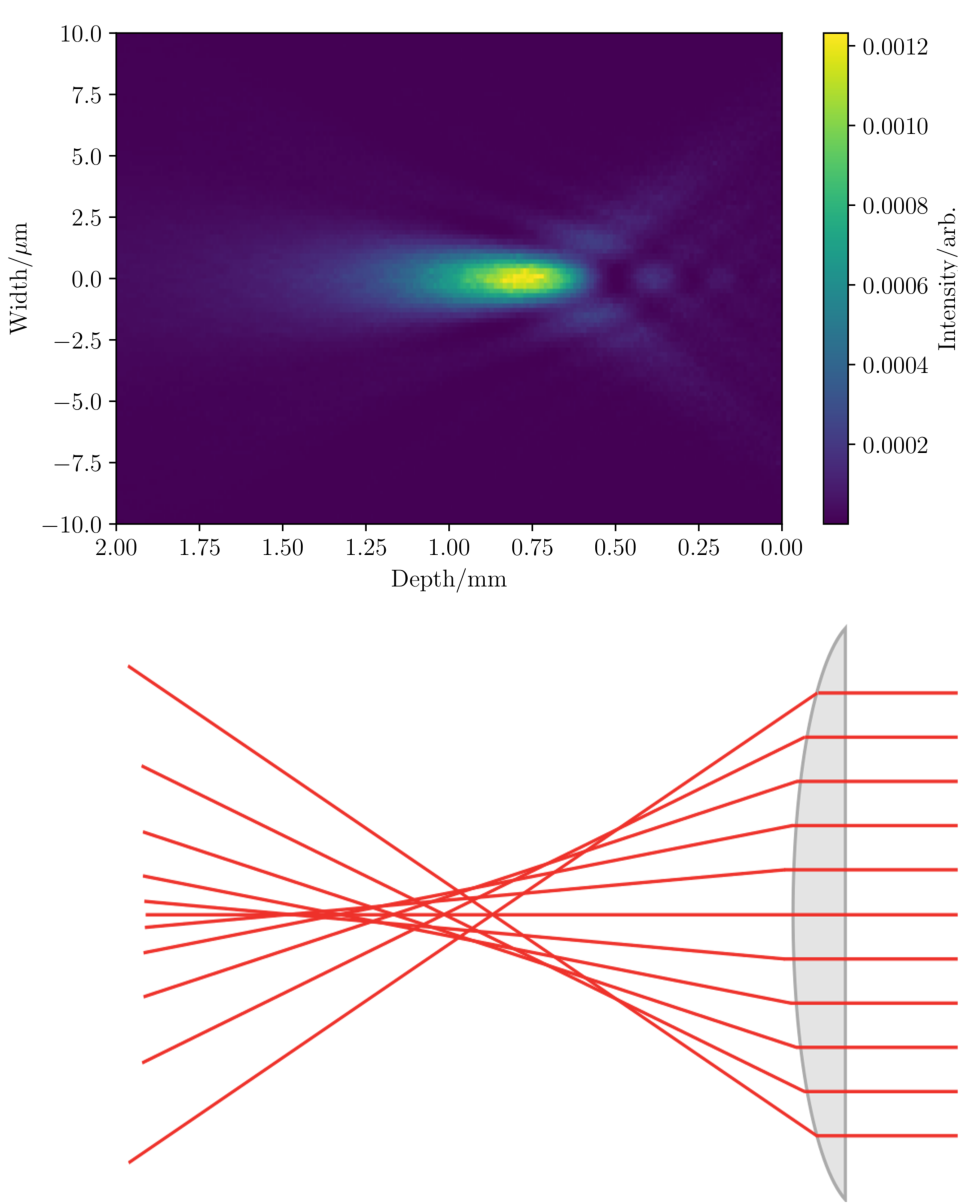
\includegraphics[width=0.65\textwidth]{spher-aber.pdf}
    \caption{Illustration of $\varphi MC$'s ability to model spherical aberrations. Top image generated using same setup as in~\cref{fig:gausssetup}, but with $D=1.5~mm$ within $\varphi$MC. Image shows the elongated focus and characteristic interference pattern behind the focus. Bottom image shows illustration of rays traced through a lens which suffers from spherical aberration.}
    \label{fig:spheraberr}
\end{figure}


This section has shown that Gaussian beams, and their physical phenomena can be accurately modelled using $\varphi MC$.
A convex-plano lens was used to focus a Gaussian beam, but it is simple to implement other lenses given a triangulated mesh of the lens or an equation that describes the shape of the lens, e.g an aspheric lens.
\FloatBarrier

\section{Bessel Beams}

Bessel beams have been the subject of intense research since their discovery in 1987~\cite{durnin1987diffraction,durnin1987exact}. 
Durnin noticed that the solution to the Helmholtz equation of the Bessel type were independent of the direction of propagation.
This means that the central core of the beam is generally more diffraction resistant when compared to a Gaussian beam with a similar spot size.
Bessel beams also have a property of ``self-healing'', this means if an obstruction is placed in the path of the central lobe of the Bessel beam, the Bessel beam can then ``heal'' and reform past the obstruction~\cite{mcgloin2005bessel}.
However, it is physically impossible to create a ``real'' Bessel beam, as the Bessel beam can have infinite rings, which each carry the same amount of power, thus would require infinite amount of power~\cite{durnin1987diffraction}.
Therefore all Bessel beams that are created experimentally are quasi-Bessel beams which are similar to their theoretical counterpart over a finite distance~\cite{durnin1987diffraction}.


These two properties make Bessel beams an attractive avenue of research, as novel solutions to imaging problems.
There is also some debate among physicists as to whether these phenomena are justly labelled, or if they glib terms used to make Bessel beams seem better than they are~\cite{debeer1987comment,harvey1984spot,durnin1987reply,sprangle1991comment,durnin1991durnin}.

\subsection{Theory}
As before with the Gaussian beam, the theory behind the Bessel beam must be discussed before we can model the beam in $\varphi MC$.
The electric field can be described using~\cref{eqn:besselEfield}~\cite{vcivzmar2006opticke}:

\begin{equation}
    E(r,z)=E_0\sqrt{\frac{2\pi k z w_0\sin(\beta)}{z_{max}}}\ \text{exp}^{\left(-\frac{z^2}{z_{max}^2}-\frac{i\pi}{4}\right)}\ J_0\left(kr\sin(\beta)\right)\ \text{exp}^{\left(ikz\cos(\beta)\right)}
    \label{eqn:besselEfield}
\end{equation}

\noindent Where:

    \indent $k$ is the wavevector, $k=\tfrac{2\pi}{\lambda}$ [$m$];

    \indent $z$ is the propagated distance [$m$]; 

    \indent $\beta$ is the angle the wavefront propagates at (see~\cref{fig:besselgeo}) [$rad$]; 

    \indent $w_0$ is the $\tfrac{1}{e^2}$ width of the input Gaussian beam [$m$]; 

    \indent $J_0$ is the Bessel function of the first kind, zeroth order; 

    \indent $r$ is radial distance from the optical axis [$m$]. 

\medskip


~\Cref{eqn:besselEfield} gives the electric field for a Bessel beam. The intensity can be calculated using:

\begin{equation}
    I(r,z)=\frac{c\epsilon_0\left|E\right|^2}{2}
    \label{eqn:besselintsub}
\end{equation}

Using the definition total power transmitted by a beam as:

\begin{equation}
    P=\frac{\pi I_0w_0^2}{2}
    \label{eqn:pwrdef}
\end{equation}

Where $I_0$ is defined as on axis intensity of the incident Gaussian beam.

\begin{equation}
    I_0=\frac{c\epsilon_0E_0^2}{2}
    \label{eqn:intdef}
\end{equation}

Substituting~\cref{eqn:besselEfield,eqn:intdef,eqn:pwrdef} into~\cref{eqn:besselintsub} yields:

\begin{equation}
    I(r,z)=\frac{4k_rP}{w_0}\frac{z}{z_{max}}J_0^2\left(k_r\ r\right)\text{exp}^{\left(-\frac{2z^2}{z^2_{max}}\right)}
    \label{eqn:besselInt}
\end{equation}


\noindent Where:

    \indent $k_r$ is the radial wavevector, $k_r=k\ sin(\beta)$;

    \indent $P$ is the power of the incident Gaussian beam.

    \medskip

A Bessel beam can be formed by an axicon lens (see~\cref{fig:besselgeo}) or by diffraction through a ring, or through the use of a spatial light modulator.
All the simulations of Bessel beams in this thesis use the axicon method of generating a Bessel beam, thus only axicons will be discussed.
\Cref{fig:besselgeo} shows the geometry of a Bessel beam formed by an axicon.
Using simple geometry and Snell's law the following equations can be derived to describe various properties of a Bessel beam formed by an axicon~\cite{merola2012characterization}.

The propagation depth of a Bessel beam is defined as the distance from the tip of the axicon to the end of the ``Bessel region''. However, in reality the Bessel beam will continue to propagate slightly passed this depth.
~\Cref{eqn:besselzmax} shows the propagation depth of a Bessel beam where $cot$ is the cotangent function ($cot x = \tfrac{1}{\tan x}$).
\begin{equation}
z_{max}=R\left(cot\left(\beta\right) - tan\left(\alpha\right)\right)
\label{eqn:besselzmax}
\end{equation}

The propagation angle of the conical waves, $\beta$ can be calculated using Snell's law and $\alpha$ the angle of the axicon:

\begin{equation}
\beta = arcsin\left(n\ sin\left(\alpha\right)\right)-\alpha
\label{eqn:betaangle}
\end{equation}

The central core of a Bessel beam is defined as the distance to the first zero of the Bessel beam.
\Cref{eqn:coreradius} shows the radius of the core, where $2.405$ is derived from the position of the first zero of the Bessel function.

\begin{equation}
r_o = \frac{2.405}{k\ sin\left(\beta\right)}
\label{eqn:coreradius}
\end{equation}

Finally, the spacing between Bessel beam rings is:
\begin{equation}
\Delta \rho = \frac{\lambda}{2\ sin\left(\beta\right)}
\end{equation}

\subsection{Validation}

To ensure that the method described in~\cref{sec:bestheory} works as intended for Bessel beams several tests are compared to theoretical expressions and experimental data.
\begin{figure}[!htbp]
    \centering
    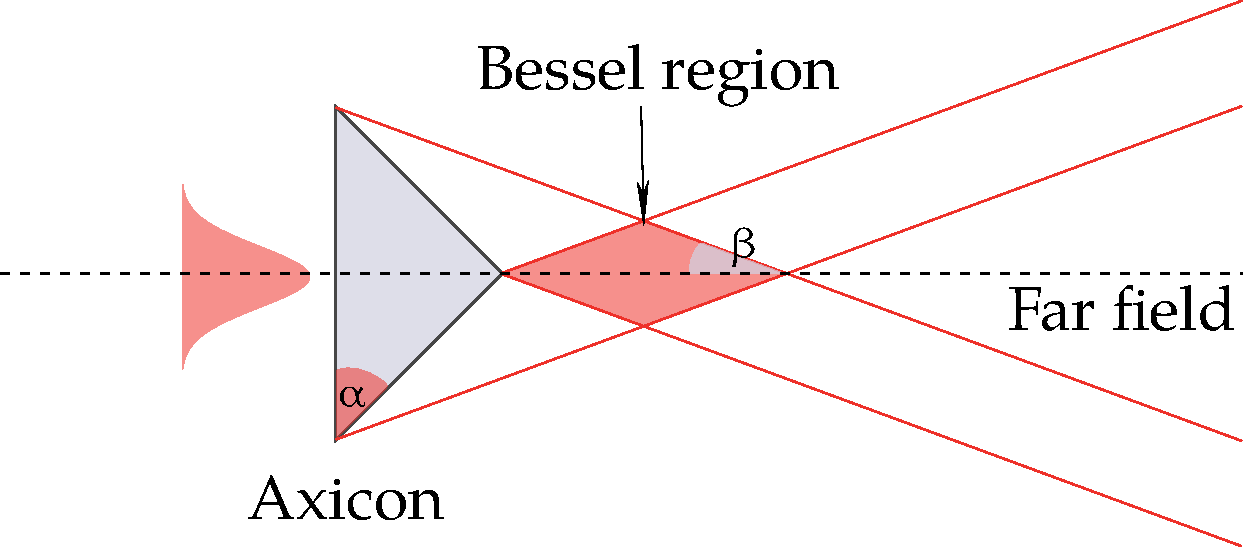
\includegraphics[width=0.5\textwidth]{bessel.pdf}
    \caption{Geometry of a Bessel beam, generated by an axicon lens. $\beta$ is the angle with the optical axis, and the angle of the conical waves. $\alpha$ is the axicon angle.}
    \label{fig:besselgeo}
\end{figure}

\subsubsection*{Comparison to a theoretical Bessel beam}

To compare with a theoretical Bessel beam, a Bessel beam is modelled in $\varphi MC$, and propagated through air into the ``Bessel region'' and then propagated into the far field to ensure the beam follows the theory in both these regions.

\Cref{fig:besselgeo} shows the set-up for the \textit{in-silico} experiments.
The Bessel beam is created with an axicon (conical) lens with an opening angle ($\alpha$) of $5^{\circ}$, and a radius of $12.7~mm$.
The input beam is Gaussian in profile with a $\tfrac{1}{e^2}$ diameter of $1~mm$, and a wavelength of $488~nm$.
The Bessel beam is then propagated to a detector screen $10~mm$ away from the tip of the axicon, which is in the middle of the ``Bessel region'' for the first test.
For the second test the Bessel beam is propagated past the ``Bessel region'' into the far field.
The detector screen has a size of $40~\mu m$ $\times$ $40~\mu m$ with a bin resolution of $1~\mu m$.
$8\times 10^{10}$ photon packets were simulated taking $\sim$ 1 hour on an 8 core Intel Xeon 3.5Ghz machine.


~\Cref{eqn:besselInt} gives the profile of a theoretical Bessel beam at a depth $z_{max}$, this is plotted against the simulation setting the various constants to (see~\cref{eqn:normalise}), with the simulation similarly normalised to the maximum intensity of the image generated. ~\Cref{fig:besselCompare} shows this comparison.

\begin{equation}
\tfrac{4k_rPz}{w_0z_{max}}e^{-2\left(\tfrac{z}{z_{max}}\right)^2}=1
\label{eqn:normalise}
\end{equation}


\Cref{fig:farfield} shows the profile of the Bessel beam in the far field, where the theory predicts it becomes a ring.
$\varphi$MC can also model the self-healing property of Bessel beams, this is shown in~\cref{fig:selfheal}.



\begin{figure}[!htbp]
    \centering
    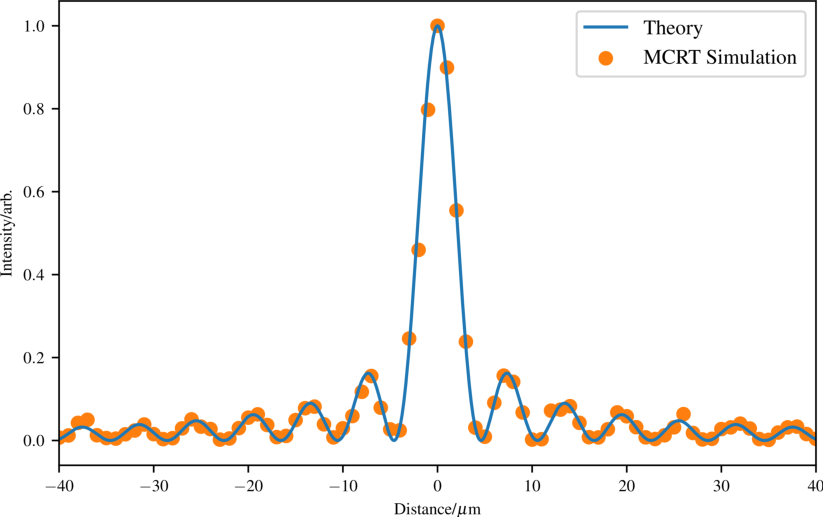
\includegraphics[width=0.65\textwidth]{compare-theory.pdf}
    \caption{Comparison of theoretical and MCRT simulation of a Bessel beams, with intensity normalised. The results from $\varphi MC$ show good agreement with the theory.}
    \label{fig:besselCompare}
\end{figure}

\begin{figure}[!htbp]
\centering
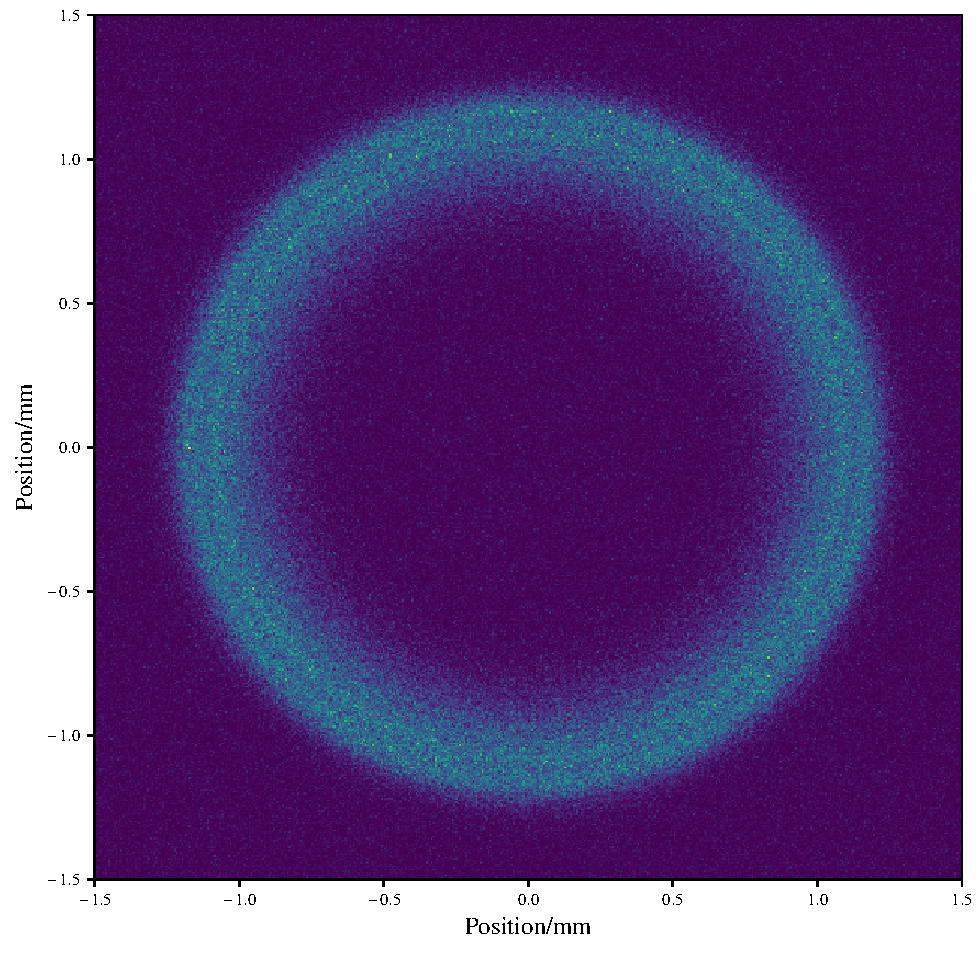
\includegraphics[width=0.5\textwidth]{farfield.pdf}
\caption{Bessel beam in the far field. Bessel beams in the far field become ring beams. Image shows a slice of intensity through the medium.}
\label{fig:farfield}
\end{figure}


\subsubsection*{Comparison to experimental data}

To ensure our algorithm works in turbid media, experiments were carried out by our collaborators, S. Reidt \textit{et al.}, at the University of Dundee.
These experiments allow us to test our algorithms ability to simulate scattering of Bessel beams in turbid media.
S. Reidt \textit{et al.} carried out an experiment where a Bessel beam was propagated through a medium of varying turbidity.
A laser, wavelength $488~nm$, with a Gaussian profile is shone on an axicon lens, with angle $5^{\circ}$.
The laser beam had a $\tfrac{1}{e^2}$ diameter of $2~mm$. 


The Bessel beam was allowed to propagate through the air for $10~cm$ before entering a cuvette of side $2~mm$.
The cuvette was filled with $500~\mu L$ of water, and various volumes of a scattering agent added.
\FloatBarrier

\begin{figure}[!htbp]
\centering
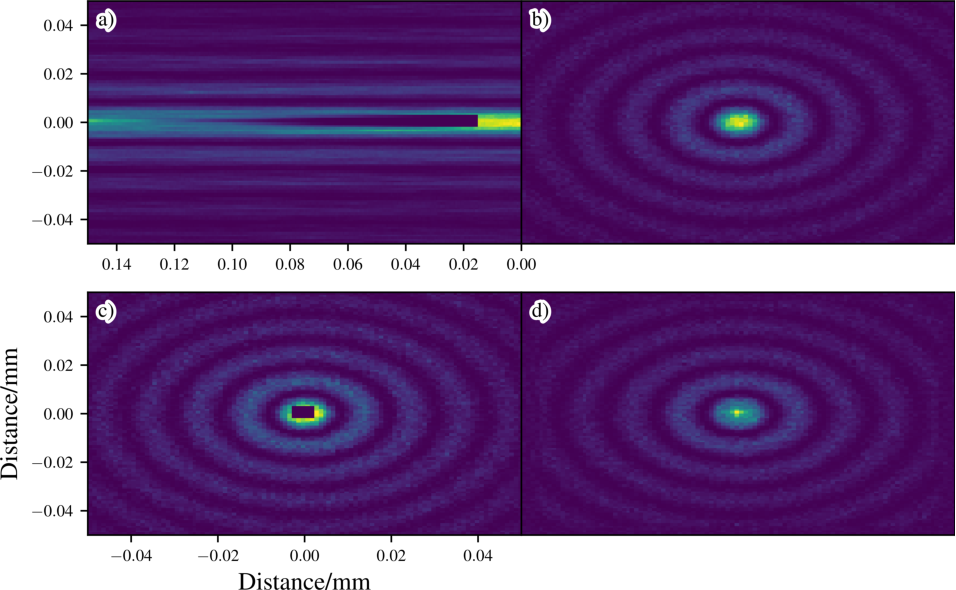
\includegraphics[width=0.75\textwidth]{selfheal.pdf}
\caption{Illustration of the Bessel beams self-healing property. Highly absorbing cube placed near the top of the medium. Figure shows that the Bessel beam forms further down the optical axis. a) shows side on view with the obstacle at $0.02~mm$, b) shows top down view at surface of the simulated b=medium before the obstacle, c) shows top down view in the middle of the obstacle, and  d) shows the top down view after the Bessel beam has ``healed''.}
\label{fig:selfheal}
\end{figure}

The scattering agent used is intralipid $20~\%$ (Sigma-Aldrich), which is diluted as shown in~\cref{tab:intra}.
~\Cref{fig:ilscatprop} shows the optical properties of Intralipid $20~\%$.
Dilutions of Intralipid are kept below 2\% scattering particle concentration, so that the scattering exhibited by the intralipid is in the independent scattering regime\footnote{The independent scattering regime is where $g$ is dependent on the size, shape and material properties of the scattering particle, and the material properties of the bulk material, but not the number of scattering particles~\cite{aernouts2013supercontinuum,mishchenko2018independent}.}.
This allows the linear scaling of the optical properties by concentrations~\cite{aernouts2013supercontinuum,vardaki2015studying,di2011effect}.
Images of the Bessel beam as it emerges from the cuvette are taken for comparison with our algorithm.
~\Cref{fig:expsetup} shows the experimental set-up.


\begin{figure}[!htbp]
    \centering
    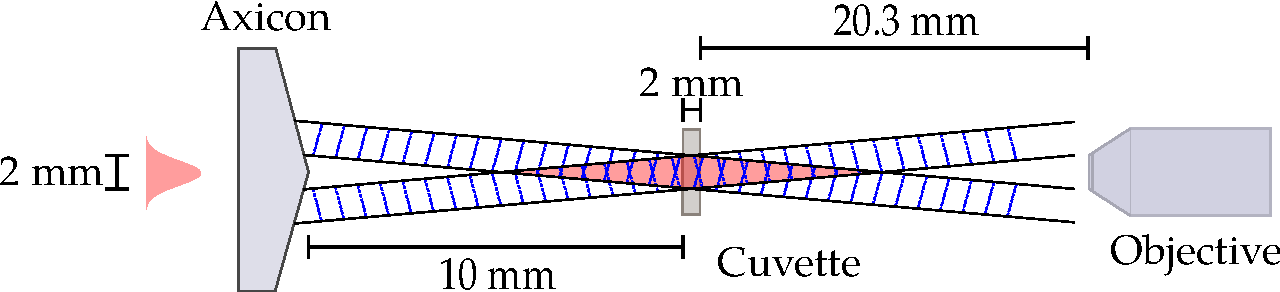
\includegraphics[width=0.8\textwidth]{bessel-exp-setup.pdf}
    \caption{Experimental set-up for propagating a Bessel beam through a cuvette filled with varying concentrations of Intralipid 20\%. Bessel beam is imaged by an $20\times$ objective lens and a Grasshopper 3 camera.}
    \label{fig:expsetup}
\end{figure}


\begin{table}[!ht]
    \begin{tabular}{cc|cc|c}
        \hline
        \multicolumn{2}{c|}{Volume/$\mu L$} & \multicolumn{2}{c|}{Intralipid concentration}                       & Optical properties              \\
        Intralipid                & $H_2O$  & Volume/\%      & Scattering particle/\%                             & Scattering coefficient/$m^{-1}$ \\ \hline
        \multicolumn{1}{c|}{0}    & 500     & \multicolumn{1}{c|}{0.00}    & 0.00                                 & 0.00                            \\
        \multicolumn{1}{c|}{2}    & 500     & \multicolumn{1}{c|}{0.39841} & 0.0908                               & 557.14                          \\
        \multicolumn{1}{c|}{4}    & 500     & \multicolumn{1}{c|}{0.79365} & 0.1816                               & 1114.28                         \\
        \multicolumn{1}{c|}{6}    & 500     & \multicolumn{1}{c|}{1.18577} & 0.2724                               & 1671.42                         \\
        \multicolumn{1}{c|}{8}    & 500     & \multicolumn{1}{c|}{1.57480} & 0.3632                               & 2228.56                         \\
        \multicolumn{1}{c|}{10}   & 500     & \multicolumn{1}{c|}{1.96078} & 0.4534                               & 2785.71                         \\
        \multicolumn{1}{c|}{12}   & 500     & \multicolumn{1}{c|}{2.34375} & 0.5448                               & 3342.84                         \\ \hline
    \end{tabular}
    \caption{Intralipid solutions used for experiment, see also~\cref{fig:ilscatprop}.}
    \label{tab:intra}
\end{table}

\begin{figure}[!htbp]
    \centering
    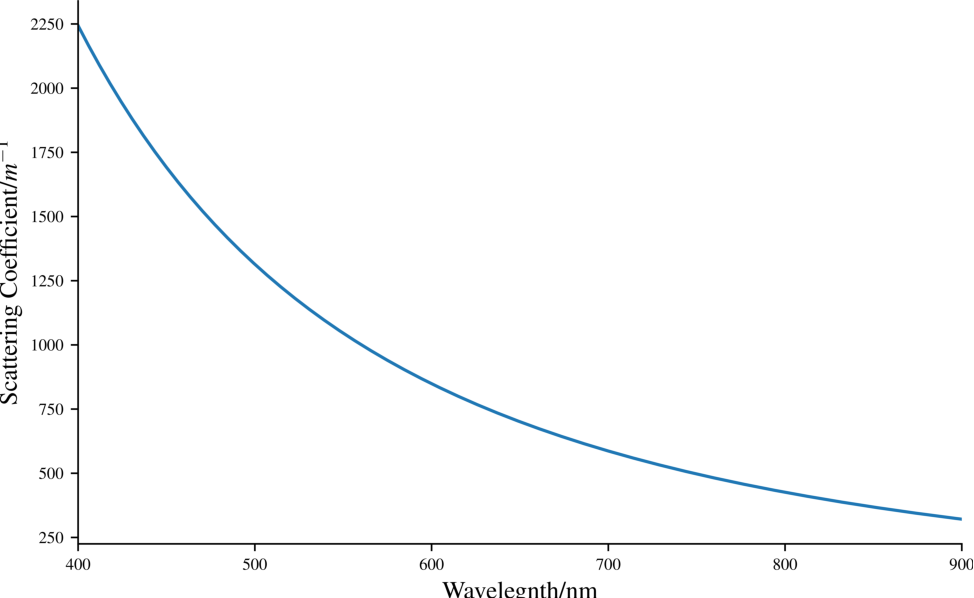
\includegraphics[width=0.5\textwidth]{scat-prop-il.pdf}
    \caption{Scattering properties of 20\% Intralipid~\cite{michels2008optical}.}
    \label{fig:ilscatprop}
    \vspace{-10pt}
\end{figure}

To model within $\varphi MC$, we simplify the experimental setup considerably.
The simulation models the propagation of photon packets through the axicon to its conical surface. 
On the conical surface the Huygens-Fresnel principle is invoked, and the packet is sampled onto the surface of the medium (cuvette).
The sampling of the photon onto the surface of the medium, speeds the algorithm up, as it does not need to simulate the photons that would ``miss'' the medium.
From there the usual~\gls*{mcrt} method propagates the packet through the medium while tracking its phase, and scattering the packet until it leaves the medium.
If the packet leaves the medium to any side other than the far side of the cuvette (e.g any side of the cuvette not facing the objective lens), then it is discarded.
If the packet leaves the medium on the objective lens facing side, then the packet is recorded by its phase onto an area element.
For each intralipid concentration $6.4\times10^{10}$ photons are run over 64 cores, taking $\sim 3$ hours for the $12\mu L$ intralipid volume.
Once all the packets have been run, the phase is converted into intensity, as in~\cref{eqn:intense}, but in 2D.

\Cref{fig:compareexpbessel,fig:compareexpbesselLine} show the results from the experiment and simulation. The simulation shows good agreement with experimental data within experimental and simulation uncertainty.

\begin{figure}[!htbp]
\centering
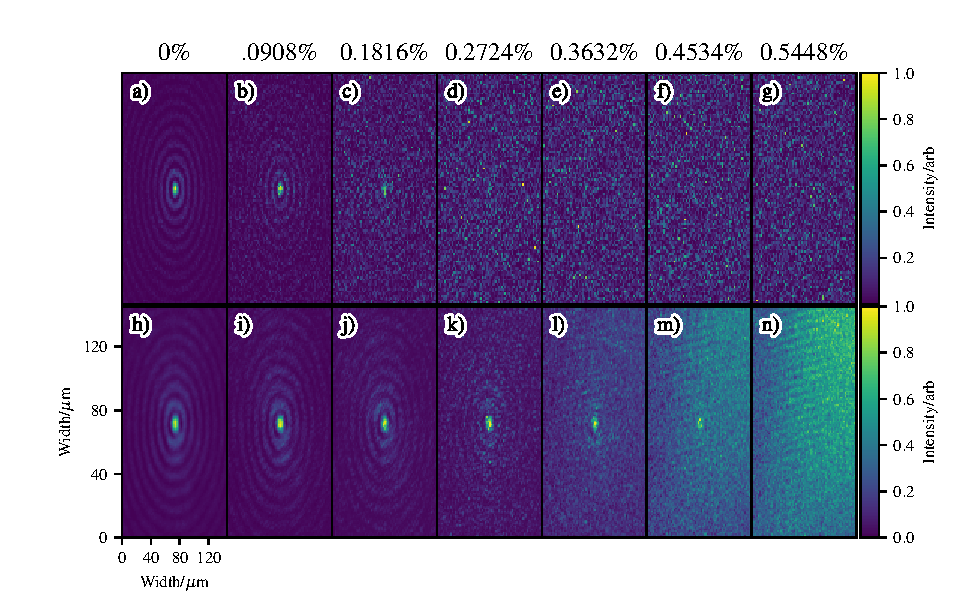
\includegraphics[width=0.95\textwidth]{compare-exp.pdf}
\caption{Comparison of experimental and simulation data for propagation of a Bessel beam produced by an axicon, through mediums of various turbidity. Images a) to g) is the data from $\varphi MC$, and h) to n) are the experimental data. Volumes along the top are the volume of Intralipid in each solution as in~\cref{tab:intra}. All images are cropped so they are the same size and normalised to the maximum value in each image.}
\label{fig:compareexpbessel}
\end{figure}

\begin{figure}[!htbp]
    \centering
    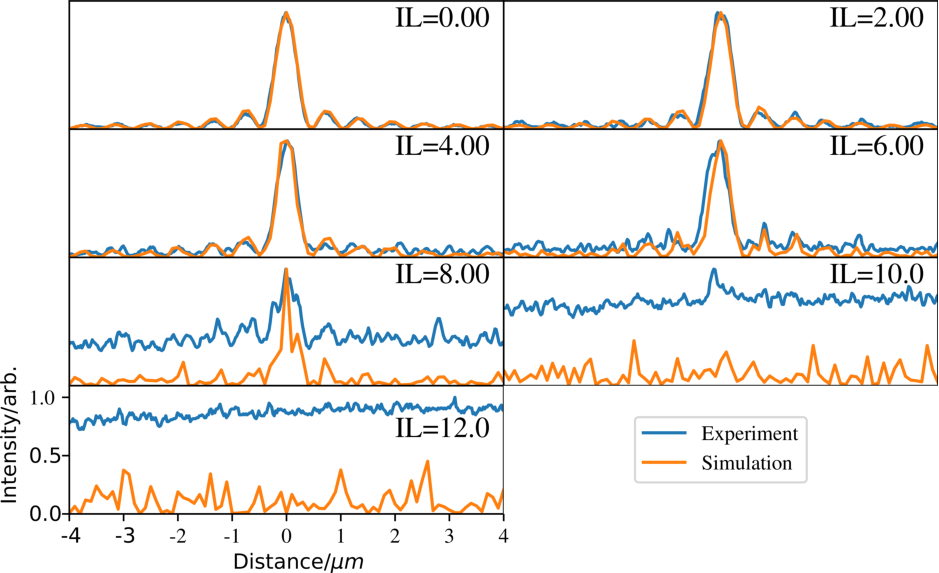
\includegraphics[width=0.75\textwidth]{Exp-sim-lineplots.pdf}
    \caption{Line graph plots of slices taken through the generated and experimental images as shown in~\cref{fig:compareexpbessel}.}
    \label{fig:compareexpbesselLine}
\end{figure}

\subsubsection*{Discussion}

As mentioned in previous sections, the power of the \gls*{mcrt} method is that we can track virtually any quantity in the simulation.
Alongside generating intensity images, we can also track the average number of scattering per packet, a quantity that is hard to measure experimentally.
\Cref{tab:numscatt} shows the average number of scattering per packet alongside the optical depth of the medium from the source to the image plane.
The simulations show that above $\approx$ 2 scatterings of a packet the Bessel beam is ``destroyed'' and the generated image becomes washed out with noise.

\begin{table}[!ht]
    \centering
    \begin{tabular}{c|c|c}
    Volume IL/$\mu L$ & Avg \# scatterings & Optical depth \\ \hline
    2      & 0.734              & 1.114         \\
    4      & 1.225              & 2.229         \\
    6      & 1.594              & 3.342         \\
    8      & 1.899              & 4.457         \\
    10     & 2.168              & 5.571         \\
    12     & 2.417              & 6.686        
    \end{tabular}
    \caption{Average number of scattering per packet and the optical depths for different volumes of Intralipid.}
    \label{tab:numscatt}
\end{table}

Originally the medium was modelled as in the experiment, a $2~mm^3$ volume.
The image created was thus a $2001 \times 2001$ with a resolution of $1~\mu m$.
To achieve a good signal to noise ratio for this set-up $6.4\times10^{12}$ packets needed to be run, taking $\sim$ 70 hours on a computer cluster using 64 cores.
This was sufficient to get a good signal to noise ratios for all the simulations up to $6~\mu L$.
However, the number of packets needed to get a good signal to noise ratio for $8~\mu L$ and above was prohibitively computationally costly.
Therefore the modelled medium was shrunk in the \textit{x} and \textit{y} directions giving: $0.5~mm \times 0.5~mm \times 2.0~mm$.
This allowed a smaller image (501 $\times$ 501), whilst keeping the same resolution.
Shrinking the medium also has the benefit that the photons are confined closer to the image plane, thus ensuring more photons hit the plane in comparison to the larger medium. 

Shrinking the mediums size does have some drawbacks.
First the Bessel beams propagation depth rely on the input beams width (see~\cref{eqn:besselzmax}).
The input beams width was kept constant between the shrinking of the volumes size.
However, shrinking the mediums size in the \textit{x} and \textit{y} directions gives the same effect as using a smaller input beam.
Therefore, the \textit{x} and \textit{y} dimension were carefully chosen such that the Bessel beam would still form a Bessel beam at the image plane.
The second issue with shrinking the medium is that some packets may be lost.
This means that in the larger medium a packet may scatter towards an \textit{x} or \textit{y} medium wall and then scatter back into the centre of the medium and then is recorded.
However, this same packet in the smaller medium would be lost as the packet would exit the medium and cease to be tracked.
It is not expected that this will cause much of an issue as any scattering event already degraded the quality of the beam, as that packet is no longer coherent with the rest of the packets, thus it will not contribute positively to the Bessel beam.
To ensure this is not an issue, results from a larger medium are compared to that of the smaller medium in~\cref{fig:compareBigSmall}.
The larger and smaller medium yield the same results (within Monte Carlo noise) for Intralipid volumes less than $8~\mu L$.
At $8~\mu L$ the smaller medium has a Bessel beams central core, whilst the larger medium is noisy, and forms no Bessel beam.
This test has shown that shrinking the medium allows accurate modelling of the propagation of a Bessel beam through a turbid medium while using less computational resources.

\begin{figure}[!htbp]
    \centering
    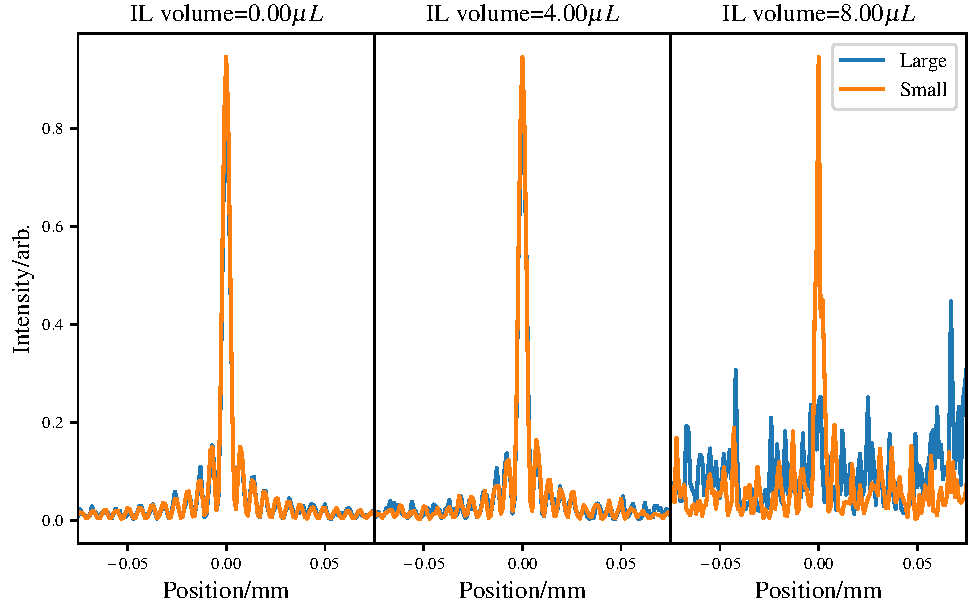
\includegraphics[width=0.7\textwidth]{compare-med-size.pdf}
    \caption{Comparison of a larger medium, $2~mm^3$ versus that of a smaller medium, $0.5~mm \times 0.5~mm \times 2.00~mm$. The figure shows that the smaller medium gives a better signal to noise ratio, whilst still accurately modelling the experiment.}
    \label{fig:compareBigSmall}
\end{figure}

\FloatBarrier

\section{Higher Order Bessel Beams}

Higher order Bessel beams (HOBBs), are Bessel beams where the electric field has an extra term of $e^{-il\varphi}$, as shown in~\cref{eqn:hobb}, and $l \neq 0$.
\Gls*{hobb} have found use for optical trapping targets that are reflective/low refractive index, and optical manipulation~\cite{garces2002transfer,garces2003observation}.
Our technique outlined in the preceding sections, can also be applied to arbitrary higher order Bessel beams. 

As before, the electric field of a $l^{th}$ order Bessel beam is:

\begin{equation}
E(r,\varphi,z)=E_0J_l(k_r r)e^{-i k_z z}e^{-i l \varphi}
\label{eqn:hobb}
\end{equation}

\noindent Where:

\indent l is the order of the beam [-];

\indent $k_{z}^{2} + k_{r}^{2} =k^2$, where $k^2$ is the wavevector [$m^{-1}$];

\indent $r$, $\varphi$, and $z$ are the cylindrical coordinates [$m$, $rad$, $m$];

\indent and $J_l$ is the l-order Bessel function of the first kind [-].

\medskip

%properties of higher order bssel beams

%methods of generating higher orders
To generate higher order Bessel beam, a helicon is used.
A helicon (shown in~\cref{fig:helix-2}) is an axicon attached to a helix phase delay element.
The helical element imparts a helical phase delay to photon packets as they pass through the element.


The distance travelled though the helicon is shown in~\cref{eqn:helix,eqn:axicon,eqn:heightdiff}~\cite{wei2015generation}.
$h_1$ is the path length travelled by a photon through the helical element.
$h_2$ is the path through an axicon, and $\Delta h$ is the height of the helical discontinuity.

\begin{align}
h_1&=\frac{l\phi\lambda}{(n-1)2\pi} \label{eqn:helix}\\
h_2&=r\ tan(\alpha)\label{eqn:axicon}\\
h_3&=h_1+h_2 \label{eqn:helicon}\\
\Delta h &= \frac{l\lambda}{n-1}\label{eqn:heightdiff}
\end{align}

Where $\phi$ is the azimuthal angle, $r$ is the radial position, $l$ is an integer that describes the order of the Bessel beam, and $\alpha$ is the axicon angle.

The path length in the above equations can be converted into a phase delay by considering the transmission functions of the individual elements~\cite{khonina1992trochoson,kotlyar2006diffraction,topuzoski2009conversion,qiong2012generalization}:
\begin{figure}[!htbp]
    \centering
    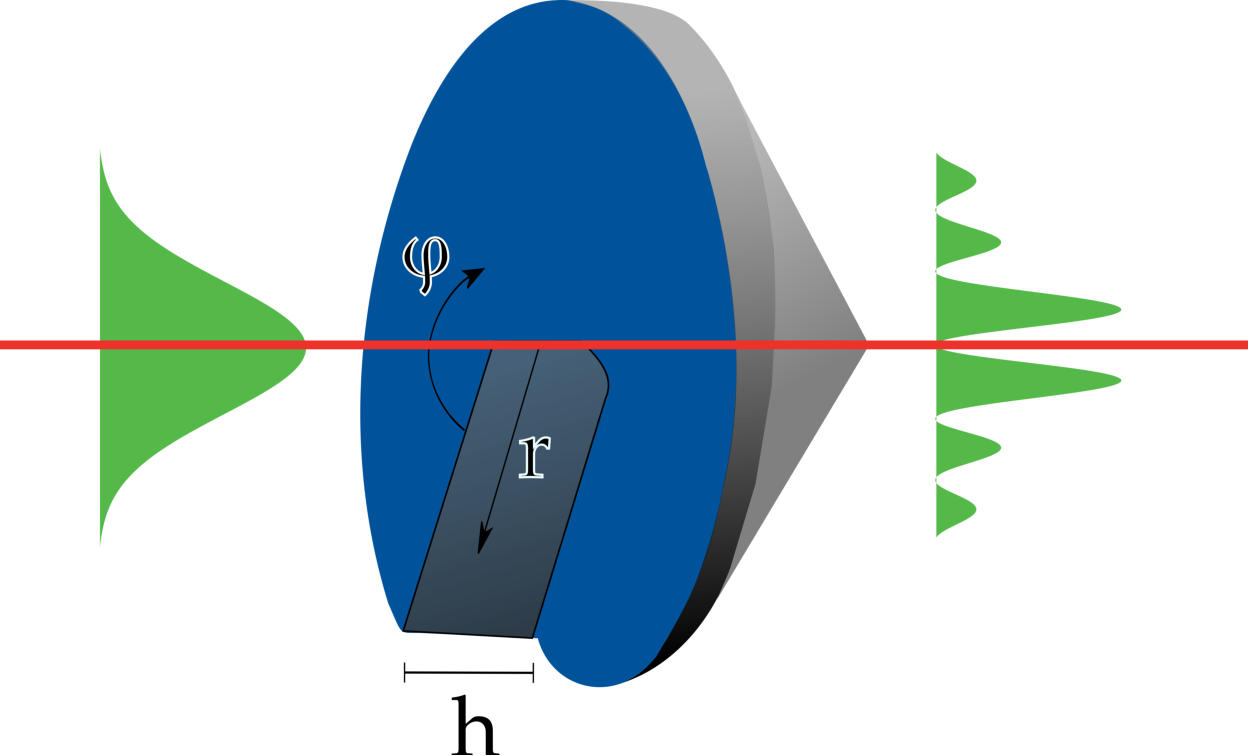
\includegraphics[width=0.4\textwidth]{helicon-2.pdf}
    \caption{Helical delay element attached to an axicon. The Axicon introduces a radial delay in addition to that of the helical element. If the input beam is a Gaussian, the output beam is a higher order Bessel beam, $l>0$.}
    \label{fig:helix-2}
    \vspace{-10pt}
\end{figure}

\begin{align}
T_1(\varphi)&=e^{-ik(n-1)h_1}=e^{-il\phi}\\
T_2(r)&=e^{-ik(n-1)h_2}=e^{-ik_rr}\\
T_3(r,\varphi)&=T_1*T_2=e^{-ik_rr-il\phi}\\
\end{align}

Where $T_1$ is the transmission function for the helical element, $T_2$ is the transmission function for the axicon, and $T_3$ is the total transmission function.
Using the small angle approximation  for $\beta$ and~\cref{eqn:betaangle}, and knowing $k_r=sin\left(\beta\right)$ yields the phase delay as a function of angle and radial position:

\begin{equation}
\varphi(\phi,r)=k(n-1)r\alpha+l\phi
\end{equation}

To implement a helicon in the $\varphi MC$ algorithm, an additional helical phase delay is added.
The additional delay is implemented by adding $l\phi$ where $0<\phi<\tfrac{2\pi}{l}$.
An actual helix element is not modelled explicitly in the code, but rather just the phase delay.
This method is similar to using a spatial light modulator in an experiment to impart a phase delay on a beam.

\Cref{fig:highordershow} shows the comparison between theoretical higher order Bessel beam and the higher order beam simulated by $\varphi MC$.



\begin{figure}[!htbp]
    \centering
    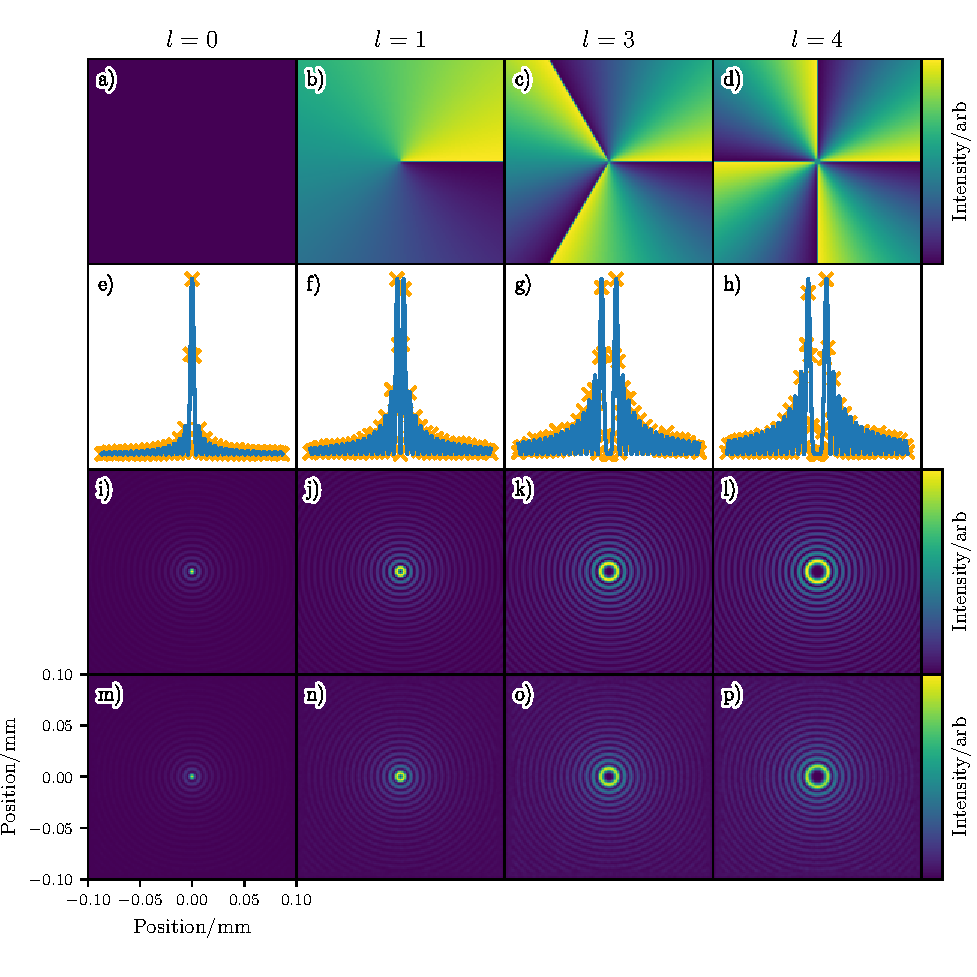
\includegraphics[width=0.85\textwidth]{higher-order-bessel.pdf}
    \caption{\Gls*{hobb}. a) to d) show the phase shift due to the helical element. e) to h) show line plots of the simulation data compared to the theory. i) to l) and m) to p) show the higher order Bessel beam images for theory and simulation data respectively.}
    \label{fig:highordershow}
\end{figure}

\FloatBarrier
\section{Comparison}
\label{sec:compBeams}
As Bessel and Gaussian beams are radically different from one another it is hard to directly compare the two beams.
Gaussian beams carry all their power in the ``central core'' of the beam, whereas in a Bessel beam, it carries the same amount of power in each ring.
Bessel beams also have a much larger depth of focus than Gaussian beams.
This section attempts to compare the two beams, to predict which beam performs better in a heavily scattering medium using $\varphi$MC\@.
Bessel beams are expected to perform better than Gaussian beams, due to their self-healing properties and non-diffractive core, this section aims to quantify how this property may or may not help penetration though a highly scattering medium. 


As mentioned, Bessel beams and Gaussian beams are not alike, so to ensure a fair comparison the Bessel beams central core width is set to that of the Gaussian beam's waist.

\begin{equation}
r_0=\frac{\kappa}{k\ sin\beta}  
\end{equation}

Where $\kappa$ is a constant that determines the metric used to measure the Bessel beam's core, and the other symbols have the same meanings as before.
For $\kappa=2.408$ the radius is measured from the maximum of the core to the first zero of the Bessel beam.
$\kappa=1.75$ measures the Bessel beam's core from the maximum to $\tfrac{1}{e^2}$ of the maximum.
For both beams central cores to be equal, the axicon used to generate the Bessel beam is adjusted.
This is achieved by calculating the ``correct'' $\alpha$ based upon the optical setup used to focus the Gaussian beam. 
Using the small angle approximation\footnote{for small $\alpha$ and $\beta$: $\beta=(n-1)\alpha$.} and $\kappa=1.75$ we can compare the Bessel beam's core radius to a Gaussian beam's waist:

\begin{align}
\frac{1.75\lambda}{2\pi sin\beta}&=\frac{2\lambda f}{\pi D} \\
\alpha &= \frac{1}{n-1}asin\left(\frac{1.75 D}{4 f}\right)
\end{align}

Where $\alpha$ is the axicon angle as before, n is the refractive index of the axicon, $D$ is the $\tfrac{1}{e^2}$ diameter of the incident Gaussian beam on the lens, and $f$ is the focal length of the lens used to focus the Gaussian beam.
Both $D$ and $f$ are properties of the optical system used to focus the Gaussian beam.
The lens used to focus the Gaussian beam is the same as used in the previous section to validate that $\varphi$MC can model a Gaussian beam, a convex-plano lens, with radius of curvature $4.6~mm$, a working distance of $8.5~mm$ and thickness of $2.2~mm$.

\medskip

The first simulation comparisons carried out between the Bessel and Gaussian beams is to use the same power to generate both beams.
The beams are then propagated through mediums of varying degrees of Intralipid solution.
Volumes of $0.0$, $26$, $52$, $78$, and $104$ $\mu L$ are used of Intralipid in 500 $\mu L$ of water.
The medium has a volume of $0.1~mm \times 0.1~mm \times 0.2~mm$, and voxel resolution of $1~\mu m$.
For both beams a wavelength of $488~nm$ and a power of $1~mW$ is used.
One hundred million packets are simulated for each simulation.
The results of this are shown in~\cref{fig:1stcomp,fig:1stcomp-1}

\begin{figure}[!htbp]
    \centering
    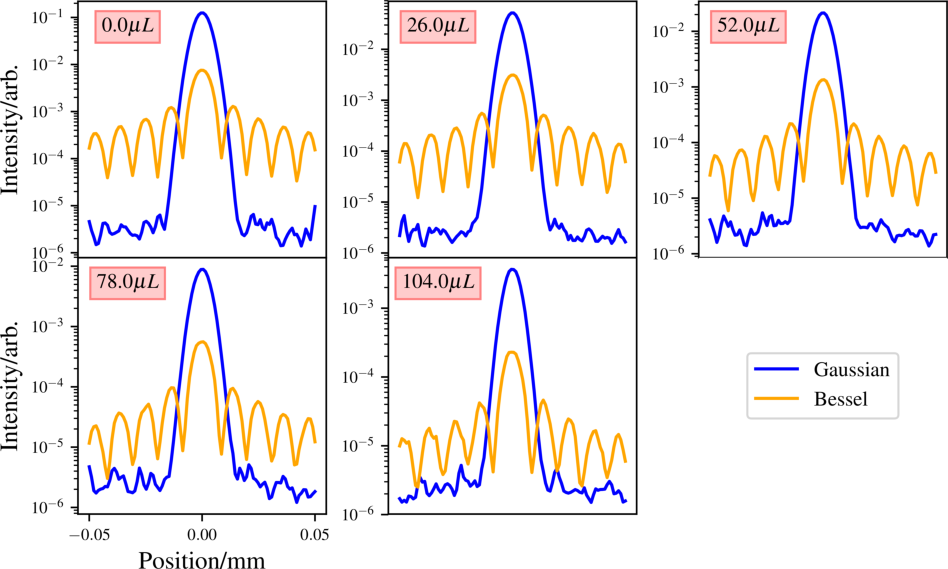
\includegraphics[width=0.75\textwidth]{Compare-BvdG-xyplane-1mW-equal-focus.pdf}
    \caption{First comparison of Bessel and Gaussian beams with equal power used to generate both beams. Plots taken at the Gaussian beams focus. The maxima at the sides of the Gaussian beam in the $0.0\mu L$plot are due to simulation effects, mainly the small size of the medium not allowing photons from further off the optical axis to interfere destructively.}
    \label{fig:1stcomp}
\end{figure}

\begin{figure}[!htbp]
    \centering
    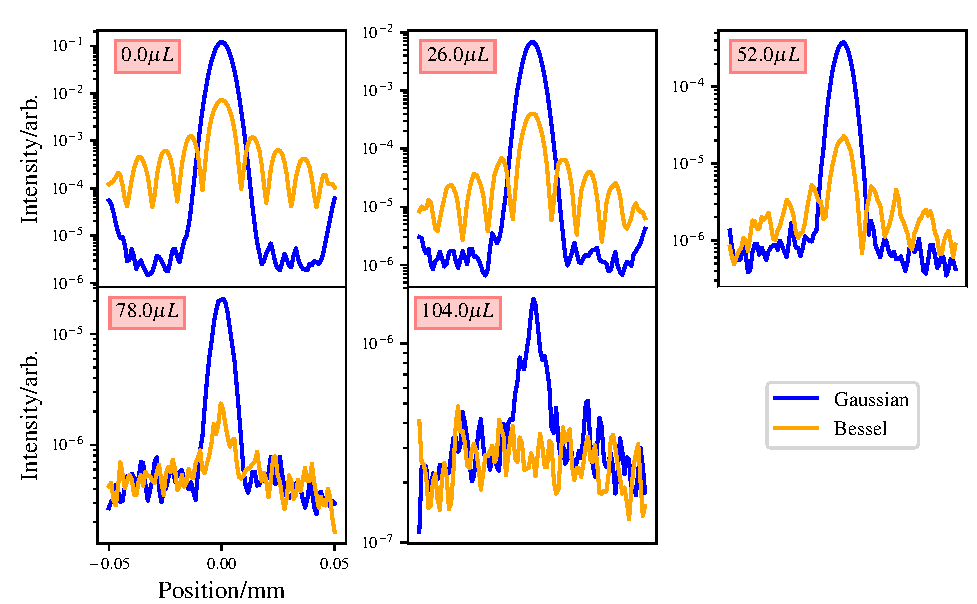
\includegraphics[width=0.75\textwidth]{Compare-BvdG-xyplane-1mW-equal-bottom.pdf}
    \caption{First comparison of Bessel and Gaussian beams, with equal power used to generate both beams. Plots taken at the bottom of the simulated medium.}
    \label{fig:1stcomp-1}
\end{figure}

The results show that for the same power, Gaussian beams propagate deeper into the medium compared to Bessel beams.
This is to be expected as in a Gaussian beam all the power is in its ``central core'', whilst the power is evenly distributed between all the Bessel beam's rings.
Therefore, for a second comparison the power given to the Bessel beam is such that the central core maximum matches that of the Gaussian beam's at its focus for the case where there is no scattering.
To achieve this the Bessel beam was given $\sim 15\times$ the power given to the Gaussian beam.
The results of this comparison are illustrated in~\cref{fig:2ndcomp}.

\begin{figure}[!htbp]
    \centering
    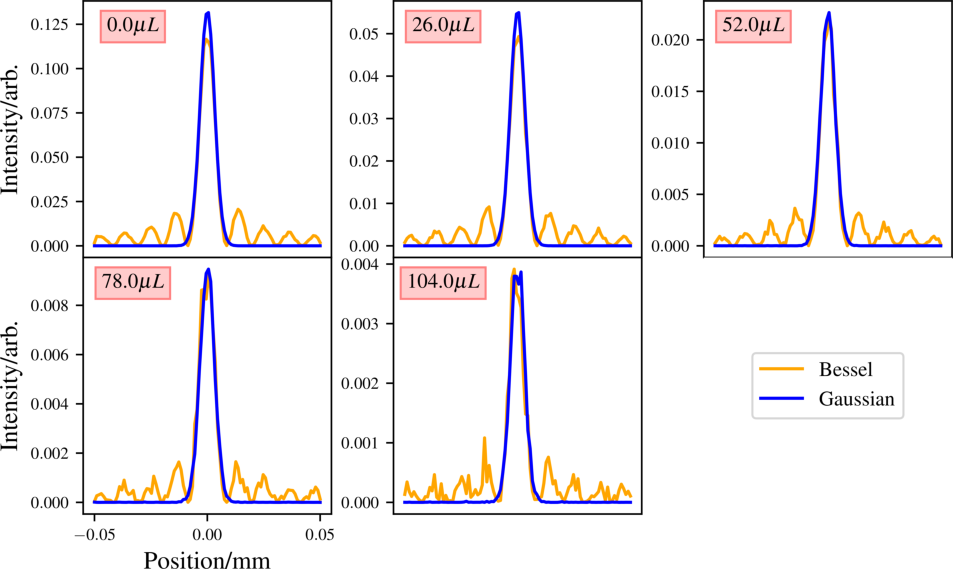
\includegraphics[width=0.75\textwidth]{Compare-BvdG-xyplane-1mW-15mW-unequal-focus.pdf}
    \caption{Second comparison of Bessel and Gaussian beams for the case where the power given to each beam, yields the same maximum at the Gaussian beams focus. These plots are taken from the Gaussian beams focus.}
    \label{fig:2ndcomp}
\end{figure}

These results show as expected that the Bessel beam now performs comparably with the Gaussian beam in lower scattering media, with a drop off in performance in the higher scattering media.

\begin{figure}[!htpb]
    \centering
    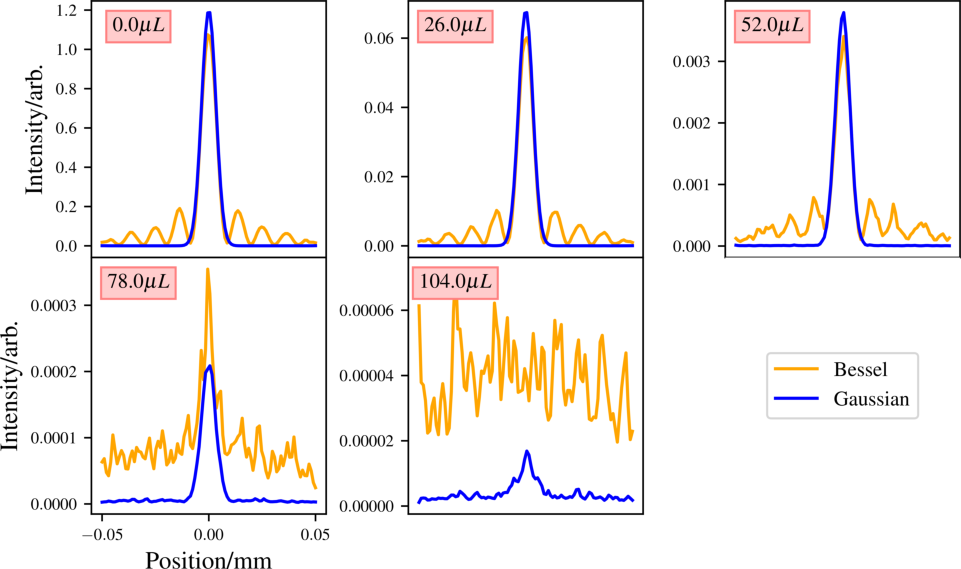
\includegraphics[width=0.75\textwidth]{Compare-BvdG-xyplane-1mW-15mW-unequal-bottom.pdf}
    \caption{Comparisons of unequal powered beams at the bottom of scattering medium.}
    \label{fig:2ncompbottom}
\end{figure}

\FloatBarrier


\subsection{Discussion}

For equal power beams in the previous section, Gaussian beams perform ``better'' in the highly scattering mediums.
Though this is expected due to the Bessel beams property that the power in the beam is spread evenly over its rings.
Thus, the power in the central lobe is much less than that of the Gaussian beam.

To give a slightly more fair comparison of intensity in the central lobes of the beams, the Bessel beam was given $15\times$ more power than the Gaussian beam. T
his allows a better comparison between the Gaussian beams' core and the Bessel beam's core and gives a more comparable intensity between the beams at the location of the Gaussian beams focus.
In this case, the Bessel beam appears to perform better in a highly scattering medium, as shown in~\cref{fig:2ncompbottom}.
The Bessel beam shows comparable intensity with the Gaussian beam in the first three mediums, though the Gaussian beam out performs the Bessel beam in the higher scattering media.
It would appear that the Bessel beams self-healing property does not help a Bessel beam propagate through a highly scattering medium.
\Cref{fig:bessel-scat-explain} shows how the Bessel beam may become degraded due to scattering.
As photons propagate though the medium they interfere with one another constructively and destructively to form a Bessel beam.
However, if enough photons are scattered, then the Bessel beam becomes degraded and thus no longer is a Bessel beam, as these photons are no longer coherent with the rest of the beam, so they act as a negative factor in the beams formation.
Another reason that the ``self-healing'' property of the Bessel beam does not ``save'' the beam from scattering is that the ``self-healing'' is not self-healing.
The self-healing in reality is just photons from further off the optical axis forming the Bessel beam further down the optical axis, e.g the photons that are impeded by the blockage are stopped, but the photons that are not impeded form a Bessel beam as expected.
If you placed a blockage in front of the Bessel beam larger than the width of the input beam, then the Bessel beam would not form at all.

Bessel beams do have their positives, their self-healing property does help ``reform'' the beam past small blockages, and their depth of field is superior to an equivalent Gaussian beam, as their central cores is ``non-diffractive''.


\begin{figure}[!htbp]
    \centering
    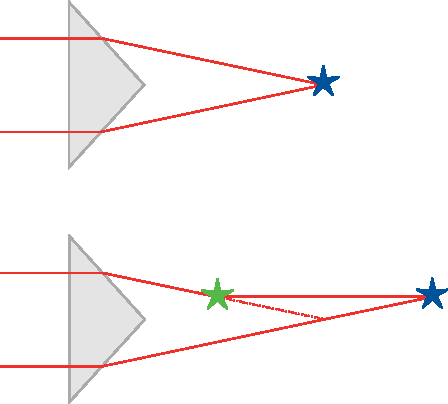
\includegraphics[width=0.5\textwidth]{bessel-scat-explain.pdf}
    \caption{Illustration of how a Bessel beam becomes degraded due to scattering. Top image shows how two photons propagate through the axicon and constructively interfere to produce a Bessel beams. Bottom image shows how scattering can affect this process.}
    \label{fig:bessel-scat-explain}
\end{figure}



\section{Conclusion}

This chapter has shown that it is possible to transform a traditional particle behaviour MCRT method into a method that allows the simulation of quasi-wave/particle behaviour of photons.
This is achieved by introducing two principles to the algorithm: the tracking of the complex phase of each packets and the Huygens-Fresnel principle.
The tracking of the complex phase of each packet allows interference of the quasi-wave/particles to be simulated.
The Huygens-Fresnel principle allows diffraction to be accurately modelled.
$\varphi MC$ has been thoroughly validated against several experiments where modelling the wave behaviour of light is vital to the experiment.
Alongside the above, presented in this chapter is the modelling of complex beam types: Gaussian and Bessel beams.
Both beam types have been validated against both theoretical and experimental results.
Finally, Gaussian beams and Bessel beams were compared with one another in a highly scattering medium, where Bessel beams appear to give better performance.
However, $\varphi$MC is not a silver bullet for modelling these complex beams in a scattering medium.
Depending on the problem at hand, the computational load can be excessive.
For example, if you want to know the intensity of the beam at all locations though a large ($> 1mm^3$) scattering medium with a complex 3D structure, then the time taken to get a good signal to noise ration may be computationally prohibitive.
Though it is expected that in most cases the intensity is not needed at all locations in a medium, and an image is all that is need to be calculated, then even in a complex 3D structure $\varphi$MC should perform better than the methods listed at the start of this chapter\footnote{Though to achieve better performance with the current code, adaptive mesh grids would have to be implemented.}.
Where $\varphi$MC excels is that it can accurately model scattering effects on the propagation of complex beams through scattering media.

%sources
%cizmar thesis
%born: principles of optics
%hecht: optics
%mignon
%prahl
%fresnel/fraunhoefer paper
%thorlabs
%sacsha thesis
%kishans papers
%various axicon papers
%aspheric papers
%phase screen model
%beam steering paper
%paper that hates on mcrt
%E-field mcrt
%\chapter{AmoebaMCRT, modelling autofluorescence in skin for novel biomarkers of cardiovascular disease}
\label{chap:salvo}
\section{Introduction}

% motivation
% explain fluro method
% explain skin model
% explain nelder mead
% explain filter choice

% results in "2d" 
% results in 3d + higher
% future work


\section{Skin Model}

So far in this thesis all tissue models have been simplified, by assuming that tissue is a homogeneous structure with uniform optical properties.
However this is not the case in reality.
Tissue is very un-homogeneous, with non-uniform optical properties.
However to create a 1 to 1 model of tissue in a simulation is impractical due to the resolution required to resolve all the constituent part of the tissue down to the cell level.
Therefore we need to make a compromise between reality and what is possible to model efficiently.
To this end the section presents a 5 layer model of human skin. 
Dermatologists usually split the skin into 5 layers: Stratum Corneum, Epidermis\footnote{The epidermis can be split into several more layers, however these layers are optical similar and are rather small so we model just one layer here.}, Papillary Dermis, Reticular Dermis, and Hypodermis, see~\cref{fig:skinexample}.

\begin{figure}[!htpb]
    \centering
    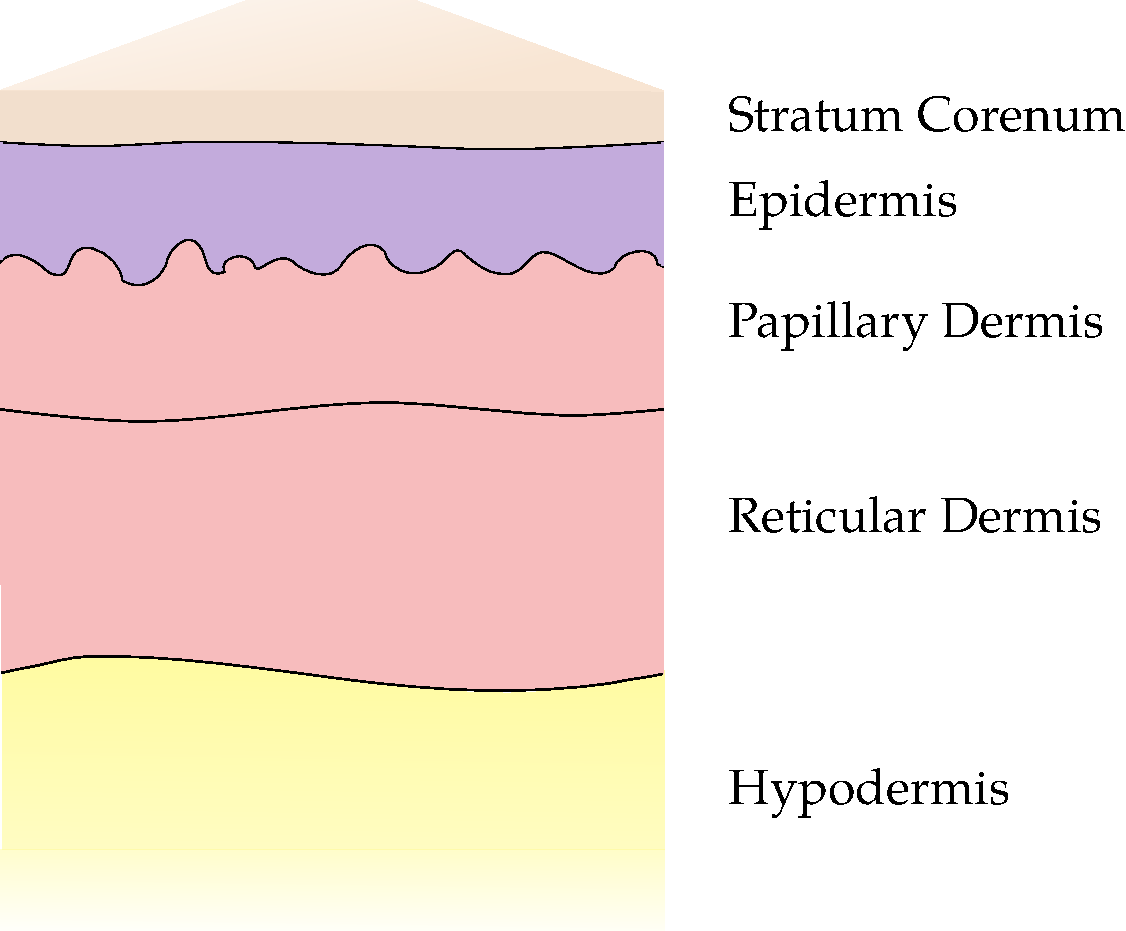
\includegraphics[width=0.7\textwidth]{Skin_layers.pdf}
    \caption{Illustration of skin layers in human skin.}
    \label{fig:skinexample}
\end{figure}

Each of these layers have various amounts of chromophores and scatterers.
To accurately model these various chromophores and scatterers, and therefore the skin, we must discuss the chemical makeup and spatial structure of the skin.

\subsection*{Stratum Corenum} % (fold)
\label{sub:stratum}

The top most layer of the skin is the stratum corenum.
This layer mostly consists of dead skin cells (keratinocytes).
The function of this layer is to be a protection barrier to prevent damage, infection and diffusion of unwanted chemicals.

% subsection stratum_corenum (end)

\subsubsection*{Epidermis} % (fold)
\label{ssub:epidermis}

Below the stratum corenum is the epidermis.
The epidermis consist of several layers that are optically similar so we restrict out model to modelling as one whole layer.
The layers that make up the epidermis are the stratum basale, stratum spinosum, stratum granulosum, and the stratum lucidum\footnote{The stratum corenum is usually part of the epidermis, however as its optical properties are different than that of the epidermis we model it as a separate layer.}.
The purpose of the epidermis is as before to provide a protective barrier to the underlying layers. 
The epidermis contains melanin which protects the stem cell keratinocyte which divide to form keratinocyte which form much of the upper layers of the skin.
In the stratum basale there is also melanocyte which produce the pigment melanin which is responsible for the color of the skin, and providing some protection from harmful UV light. 
Other types of cells found i the epidermis are Langerhans cells and Merkel cells which are part of the immune system and nervous system respectively.

% subsubsection epidermis (end)

\subsection*{Dermis} % (fold)
\label{sub:dermis}

The dermis is split into three different layers in our model: the papillary dermis, reticular dermis and the hypodermis.

The papillary dermis has blood

The reticular dermis has blood

The hypodermis consists of fat and  

% subsection dermis (end)

\subsubsection*{Optical Properties} % (fold)
\label{sub:optical_properties}

With a discussion of what makes up the skin, and what molecules contribute to the skins optical properties, this section gives an account of how our skin model, models the optical properties of skin.

To model blood, we first split blood into Deoxygenated and Oxygenated. We mix these two groups using the tissue oxygenation coefficient $S$. Blood absorption spectra are taken from%~\cite{}

\begin{equation}
\mu_{a,oxy/deoxy}=150\ \ln10\ \frac{\epsilon}{64458}
\label{eqn:oxy}
\end{equation}

\begin{equation}
\mu_{a,b}(\lambda) = SO_2\mu_{a,Oxy}+(1-SO_2)\mu_{a,DeOxy}
\label{eqn:blood}
\end{equation}

The next chromophores are bilirubin and $\beta$-carotene.
The absorption coefficients are calculated using the blah 

\begin{equation}
\mu_{a,Bilirubin}(\lambda)=\frac{\epsilon_{bilirubin}}{585}\ ln10\ C_{bilirubin}
\label{eqn:bili}
\end{equation}

\begin{equation}
\mu_{a,\beta-Caro}(\lambda)=\frac{\epsilon_{\beta-Caro}}{537}\ ln10\ C_{\beta-Caro}
\label{eqn:caro}
\end{equation}

To model melanin`'s absorption coefficient we use~\cref{eqn:eqn:melanin}, taken from...

\begin{equation}
\mu_{a,mel}(\lambda)=6.66\times10^{11} \times \lambda^{-3.33}
\label{eqn:eqn:melanin}
\end{equation}

Finally we use a base absorption coefficient to model the absorption due to the other parts of the skin that contribute to its optical properties, but individually do not have a large effect.

\begin{equation}
\mu_{a,b}=7.84\times10^{8}\times\lambda^{-3.255}
\label{eqn:base}
\end{equation}


\begin{figure}[!htpb]
	\centering
	% \includegraphics[width=0.75\textwidth]{}
	\caption{Absorption coefficients for the various chromophores found in skin.}
	\label{fig:absorcoeff}
\end{figure}





% subsubsection optical_properties (end)


\section{Modelling Fluorescence}

Fluroescene is the process in which light of a certain wavelength is incident on a molecule, the molecule absorbs the light and re-emits the light at a new longer wavelength.

\Cref{fig:Jabo} shows an example of Jablonski diagram.

\begin{figure}[!htpb]
	\centering
	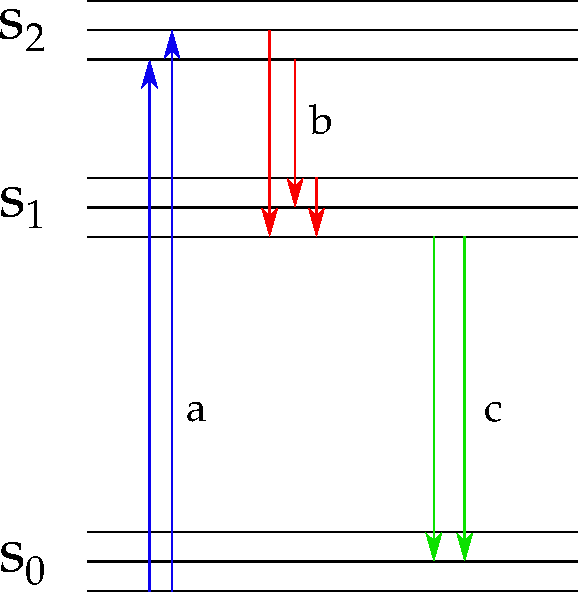
\includegraphics[width=0.45\textwidth]{jabo-diag.pdf}
	\caption{Jablonski diagram for PPIX. a) excitation of the ground state via absorption of a photon, b) non-radiative transition, and c) fluorescence.}
	\label{fig:Jabo}
\end{figure}

To model fluorescence from multiple fluorophores requires a change of the \gls*{mcrt} code presented thus far.
This change is to the interaction portion of the algorithm, so that it will now include the option for a packet to undergo fluorescence.
To calculate whether a packet absorbs, scatters or fluoresces, first the probability of each of these events must be calculated.
Discussion of scattering and absorption (by the bulk medium) was described in~\cref{sec:opticalprops}.
To calculate the probability of fluorescence, we first assume that the quantum yield of the molecule is unity.
This is physically unrealistic, however it does not affect the simulations accuracy, as modelling a realistic quantum yield would mean that more packets would be discarded, and thus the signal to noise ration would be worse than if we assume a quantum yield of unity.
To calculate the probability of fluorescence, the absorption coefficient of the florescent molecule must be calculated.
This is shown in~\cref{eqn:flurodef}:

\begin{equation}
\mu_f=\ln\left(10\right) C \varepsilon
\label{eqn:flurodef}
\end{equation}

Where $C$ is the concentration of the fluorophore, $\varepsilon$ is the extinction coefficient of the fluorophore, and $ln(10)$ is the natural logarithm of 10\footnote{This factor appears as historically $\varepsilon$ was measured in base 10~\cite{jacques2013optical}.}.\\

The next step is to calculate the total attenuation coefficient for a given species as in~\cref{eqn:totdef}

\begin{equation}
\mu_{t_i}=\mu_{s_i}+\mu_{a_i}+\mu_{f_i}
\label{eqn:totdef}
\end{equation}

Where as usual $\mu_a$ and $\mu_s$ are the absorption and scattering coefficients, and $\mu_f$ is the fluorescence coefficient as defined in~\cref{eqn:flurodef}.
As the absorption coefficient of fluorophores are small in comparison to the medium, and that the absorption coefficient of fluorescent molecules are generally much larger than that of their scattering coefficient, we assume that the scattering coefficient is negligible.
Finally we calculate the probability of interacting with a given species using~\cref{eqn:totspec}

\begin{equation}
P_i=\frac{\mu_{t,i}}{\sum\limits_{i=1}^{N} \mu_{t,i}}
\label{eqn:totspec}
\end{equation}

Where $P_i$ is the probability of interacting with the $i^{th}$ species, the numerator is the attenuation coefficient for $i^{th}$ species, and the denominator is the total attenuation coefficient for all the species.

\cref{algo:speciespick} shows the process used to determine which species to interact with.

\newpage

\begin{center}
\begin{algorithm}[H]
\SetAlgoLined
  set $\mu_{tot}$\;
  set all $P_i$'s\;
  set $\xi_1$\;
  \uIf{$\xi_1 < P_1$}{
    set $\xi_2$\;
    \uIf{$\xi_2 < a_m$}{
      Scatter in medium\;
     }
     \Else{
      Absorb in medium\;
     }
  }
  \uElseIf{$\xi_1 < P_1 + P_2$}{
    Species 1 fluoresces\;
  }
  \uElseIf{$\xi_1 < P_1 + P_2 + P_3$}{
    Species 2 fluoresces\;
  }
  \uElseIf{$\xi_1 < P_1 + P_2 + P_3 + ... + P_n$}{
    Species n fluoresces\;
  }
  \Else{
    Error\;
  }
\
\caption{\textit{An algorithm to determine which species to interact with. $P_1$ is the probability of interacting with the bulk medium, $P_2$ to $P_n$ is the probability of interacting with a fluorescent species, $a_m$ is the albedo of the bulk medium, $\xi_i$ is a random number, and $\mu_{tot}$ is the total attenuation coefficient of all the species summed.}}
\label{algo:speciespick}
\end{algorithm}
\end{center}

This method allows an arbitrary number of fluorophores to be modelled.


\section{Nelder-Mead Method}

The \gls*{nm} method is an algorithm for unconstrained optimisation. 
The algorithm is based upon iteratively updating a simplex. 
A simplex is a structure in $n-dimensional$ space, consisting of $n+1$ points that are not in the same plane. 
Therefore in 1D, the simplex is a line, in 2D a triangle, in 3D a tetrahedron, etc.. 
The Nelder-Mead method is a gradient free method, meaning that it does not require derivative to be calculated and that the search space does not need to be smooth.

The algorithm works by removing the worst vertex of the simplex and replacing it with a `better' vertex calculated via a number of different operations.
These operations can be seen in~\cref{fig:NM-operations}.

The first step of the~\gls*{nm} method is to sort the initial vertices according to their fitness.
For $n=2$, we define $x_w$ as the `worst' point, $x_l$ and the `lousy' point, and $x_b$ the `best' point, such that $f(x_b)\leq f(x_l)\leq f(x_w)$, where $f(x)$ is evaluating the `fitness' of a point $x$.
With the vertices sorted, the centroid of the simplex is calculated as in~\cref{eqn:centroid}.
The centroid is the mean of all the vertices bar the `worst' point.

\begin{figure}[!htbp]
    \centering
    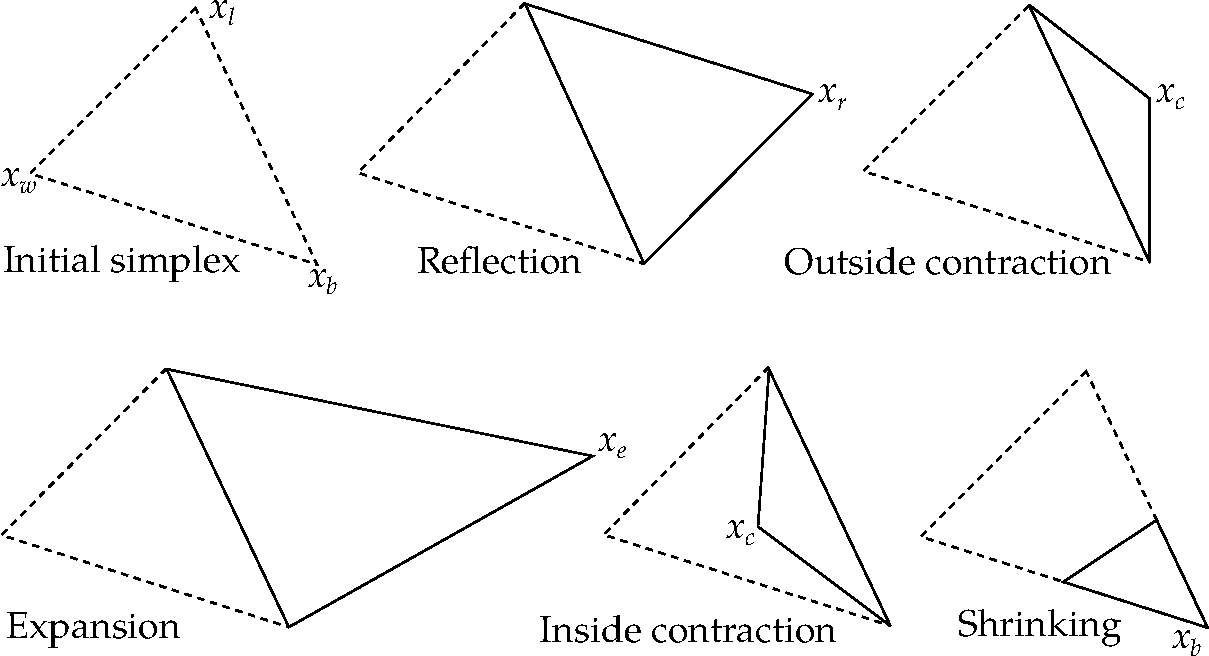
\includegraphics[width=0.75\textwidth]{simplex-operations.pdf}
    \caption{Operations that can be preformed on a simplex for $n=2$.}
    \label{fig:NM-operations}
\end{figure}

The next step is to move the simplex via a reflection.
To calculate the new vertex via reflection~\cref{eqn:reflect} is used, where $\alpha$ is the reflection factor.
If this new point, $x_r$, is better\footnote{Here better means the point has a lower fitness score, as we use $\chi^2$ metric to assess the fitness of a point.} than the current `best' point then we calculate a new point in the same direction but further using the expansion operation~\cref{eqn:expand}, where $\gamma$ is the expansion factor.
If this new point, $x_e$, is better than the `best' point then we replace $x_w$ with $x_e$ and start the process again.
However is $x_e$ is not better than the `best' point, then we discard it and replace the worst point with $x_r$ the reflected point.

If when calculating $x_r$, we find that is worse than the `best' point, we then check if $x_r$ is better than the `lousy' point.
If $x_r$ is better than $x_l$ then we replace the `worst' point and start the process again.
However if the $x_r$ is worse than $x_l$, we then compare it to the `worst' point.
If $x_r$ is better than the `worst' point then we preform and inside contraction~\cref{eqn:insidecontract}, where $\beta$ is the contraction factor.
If this new point, $x_{ic}$, is better than the `worst' point then we keep it, otherwise we preform the shrink operation, shrinking the whole simplex around the `best' point.

If $x_r$ is not worse than the `worst' point then we preform an outside contraction~\cref{eqn:outsidecontract}.
This computes a new point $x_{oc}$.
If $x_{oc}$ is better than $x_w$, then we keep it, otherwise again we shrink around the `best' point.

The process described above is summarised in~\cref{fig:NM-algo}.
Standard values for the factors are: $\alpha=1$, $\beta=\frac{1}{2}$, and $\gamma=2$.
Though in practise these values are adjusted for the problem at hand.

\begin{align}
c &= \frac{1}{n}\sum \limits_{i=1,i\neq w}^{n+1} x_i \label{eqn:centroid}\\
x_r &= c + \alpha(c - x_w)\label{eqn:reflect}\\
x_e &= c + \gamma(x_r - c)\label{eqn:expand}\\
x_{oc} &= c + \beta(x_r - c)\label{eqn:outsidecontract}\\
x_{ic} &= c + \beta(x_w - c)\label{eqn:insidecontract}
\end{align}

As the Nelder-Mead method has no inbuilt convergence criteria, this must be added.
We use two different criteria based upon simplex size, and vertex fitness.
The criteria for the simplex size is as; if the size of the simplex(~\cref{eqn:sizeof})
Where $p_i$ and $p_{i+1}$ are vertices in the simplex that are connected by and edge. 

\begin{equation}
size=\sum\limits_{i=1}^{n+1}|p_{i}-p_{i+1}|
\label{eqn:sizeof}
\end{equation}

If the size of the simplex falls below a pre-set value, then we preform a factorial test to see if the simplex should be restarted or if the algorithm should terminate.
The factorial test checks the space around the current simplex to ensure that we have converged to a global minima.
If the check fails then the algorithm is restarted with the current best point kept, and new vertices generated.

\begin{figure}[!htbp]
    \centering
    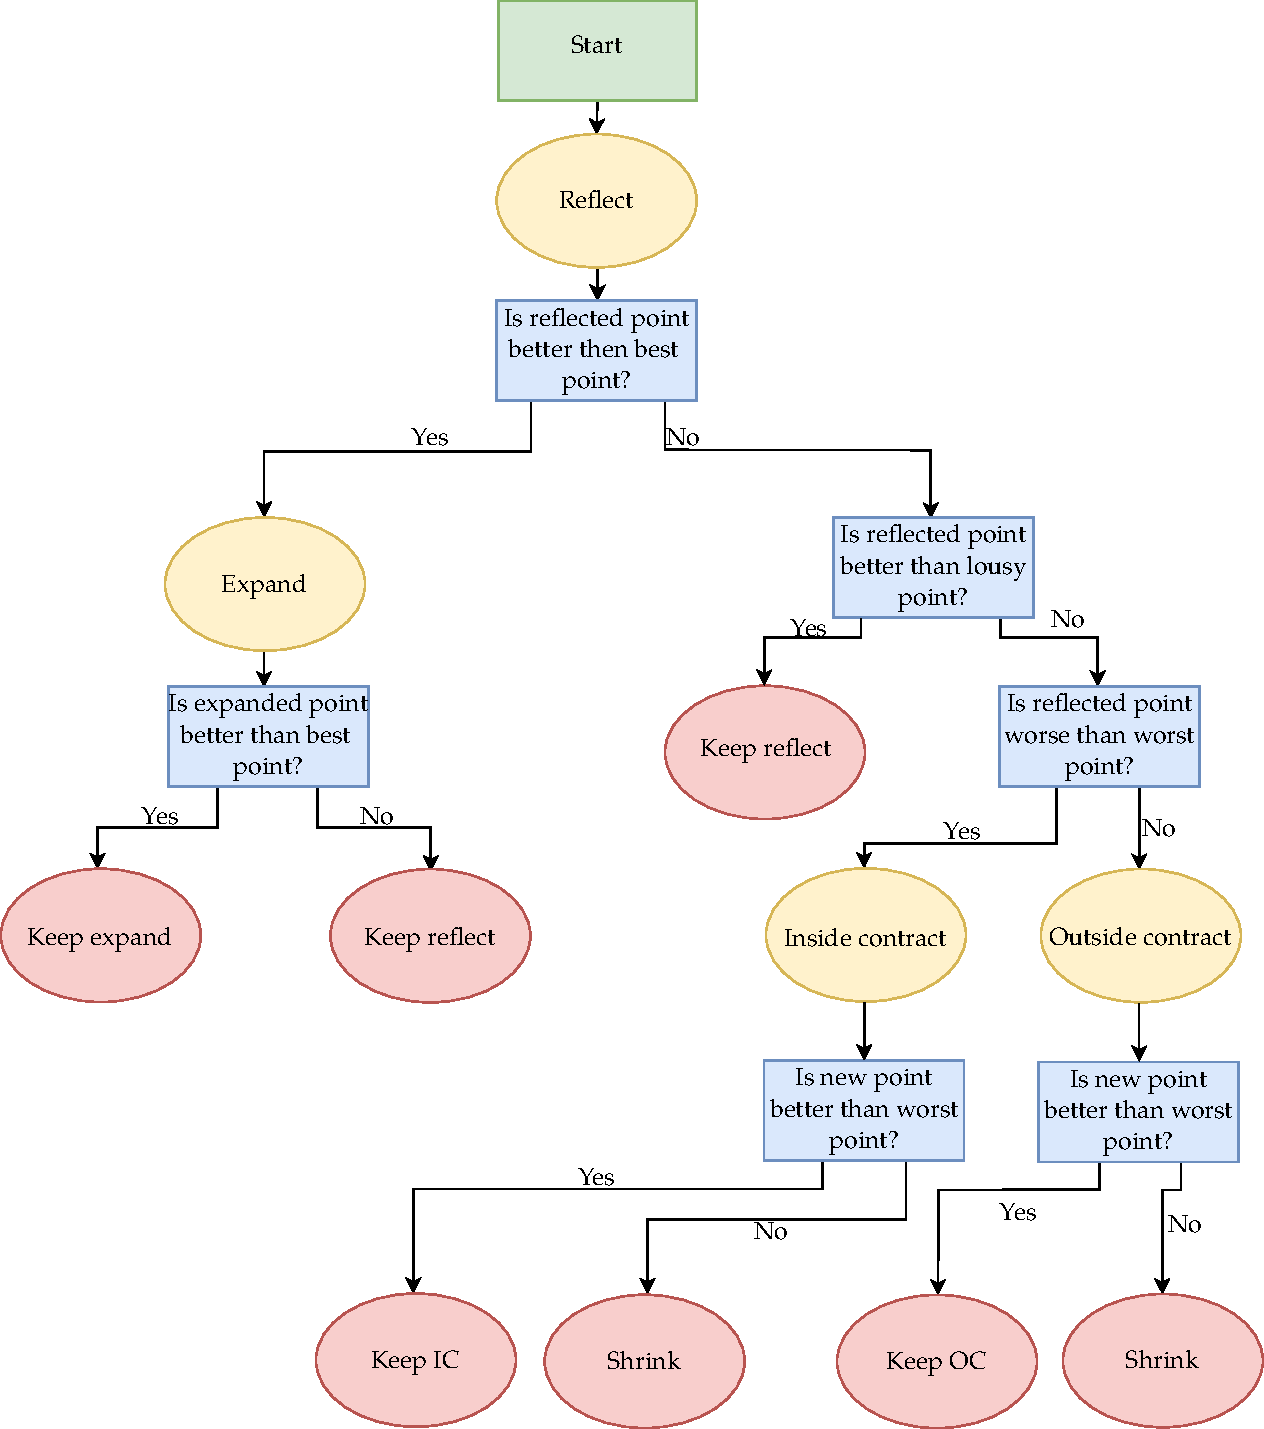
\includegraphics[width=0.65\textwidth]{flowchart.pdf}
    \caption{Nelder-Mead decision tree}
    \label{fig:NM-algo}
\end{figure}

The other convergence criteria is the a check to see if the best point is `good enough'.
The current best point is compared to a pre-set fitness value.
If the best point is better than the pre-set value then the algorithm terminates.

\FloatBarrier
\section{Validation}
The~\gls*{nm} method was coded in Fortran, so that it could be easily interfaced with the~\gls*{mcrt} code developed as part of this thesis.
To test that the method works as intended a number of trial functions were tested, see~\cref{tab:testfuncs}.
This was achieved by selecting an initial simplex, and the method allowed to iterate until it converged.
The results of this are shown in~\cref{fig:nmtest}.


\begin{table}[]
    \begin{tabular}{|c|c|c|}
    \hline
        Name         & Formula                                                                & Global Minumum                \\ \hline
        Sphere       & $x^2+y^2$                                                              & $f(0,0)=0.$                   \\ \hline
        Rosenbrock   & $(a-x)^2+b(y-x^2)^2$                                                   & $f(1,1)=0.$                   \\ \hline
        Ackely       & $ -20\exp\left[-0.2\sqrt{0.5\left(x^{2}+y^{2}\right)}\right] - $       & $f(0,0)=0.$                   \\
                     & $\exp\left[0.5\left(\cos 2\pi x + \cos 2\pi y \right)\right] + e + 20$ &                               \\ \hline
        Himmelblau's & $(x^2+y-11)^2+(x+y^2-7)^2$                                             & $f(3,2)=0., $                 \\
                     &                                                                        & $f(-2.805118,3.131312)=0.,$   \\
                     &                                                                        & $f(-3.779310,-3.283186)=0.,$  \\  
                     &                                                                        & $f(3.584428,-1.848126)=0.$    \\ \hline
    \end{tabular}
    \caption{Table of standard test functions for numerical optimisation.}
    \label{tab:testfuncs}
\end{table}


\begin{figure}[!htbp]
    \centering
    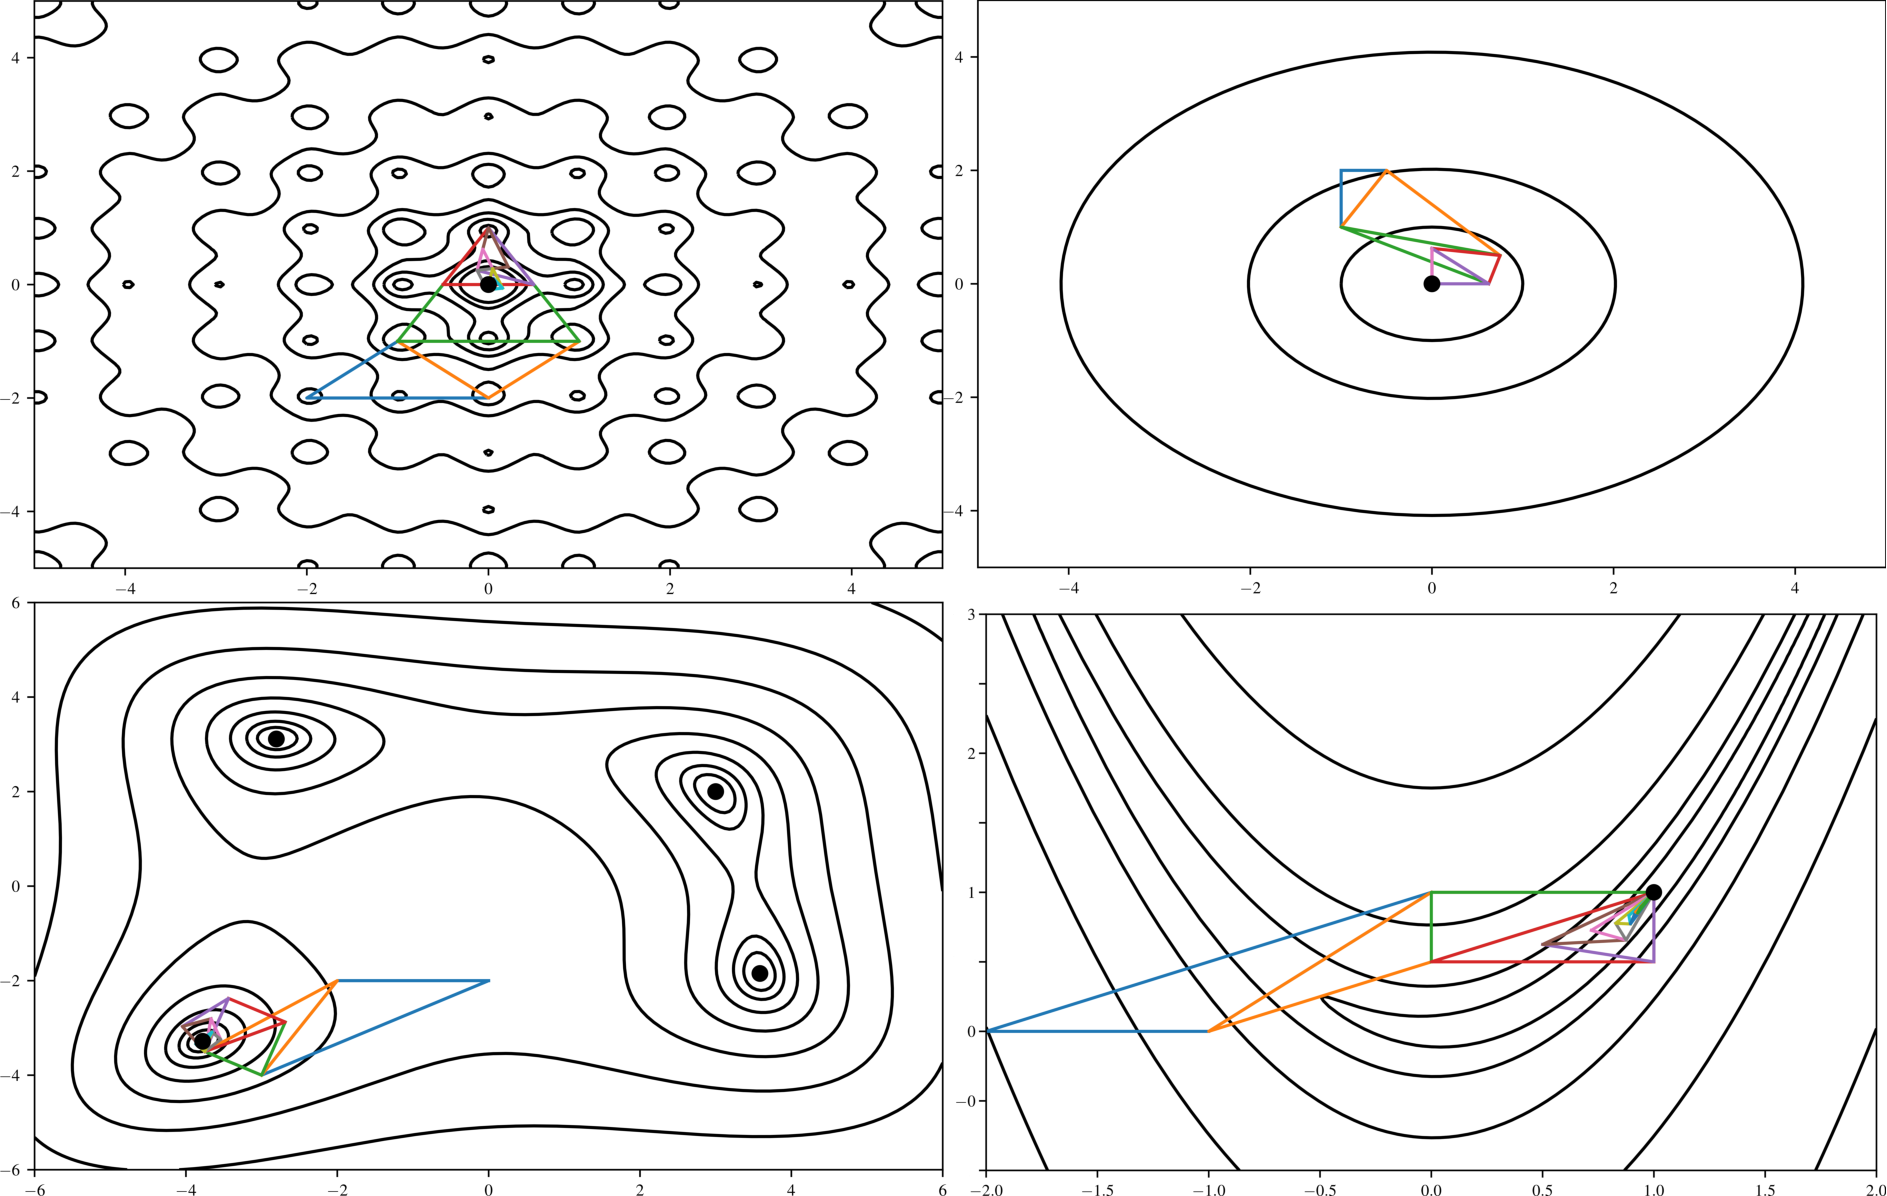
\includegraphics[width=0.75\textwidth]{all-nm-tests.pdf}
    \caption{Contour plots of test functions with Nelder-Mead simplexes over plotted. Top left is the Ackely function, top right is the sphere function, bottom left is the Himmelblau's function, and the bottom right is the Rosenbrock function. Blue simplex is the initial simplex, and the large black dots represent the Global minima.}
    \label{fig:nmtest}
\end{figure}

To ensure that the~\gls*{nm} method can be used to find the unknown concentrations of the autoflurophores, we test the method with a known model.
This model consists of three different fluorophores: NADH (nicotinamide adenine dinucleotide), FAD (flavin adenine dinucleotide), and a fictitious fluorophore that has similar properties to NADH and tyrosine, such that the excitation spectrum is that of NADH and the emission spectrum is that of tyrosine.
The three fluorophores are distributed in the stratum corenum (NADH), epidermis (FAD), and the papillary dermis (fictitious).
The concentration in these layers is such that the bulk optical properties are not affected: NADH has a concentration of $x$, FAD $y$, and the fictitious fluorophore has a concentration of $z$.

As many models need to be run in order to determine whether a global maxima has been reached using the NM method and the fluorophore concentration low many packets need to be run.
Therefore the ~\gls*{mcrt} algorithm has to be computationally efficient in order to arrive at an answer within a reasonable time.
To this end the 3D skin model is shrunk to a 1D model so that the optical integration routine can efficiently move the photon through the simulated medium.
The optical properties of the incident wavelength are also stored so that when a new photon is started the optical properties can easily be adjusted without need for any calculation.


\begin{figure}[!htbp]
	\centering
	\includegraphics[width=0.6\textwidth]{target-toy.pdf}
	\caption{Example of toy model for testing NM method. The three peaks correspond to the fictitious fluorophore, NADH, and FAD respectively.}
	\label{fig:figure1}
\end{figure}

We first run this model through the MCRT to get an output spectrum.
We then test the~\gls*{nm} method for $n=2$ and $n=3$.

\section{Results}

\begin{figure}[!htpb]
    \centering
    \includegraphics[width=0.75\textwidth]{UV-fluence-365nm.pdf}
    \caption{Penetration of UV radiation as a function of depth.}
    \label{fig:uvpen}
\end{figure}

\begin{figure}[!htpb]
    \centering
    \includegraphics[width=0.75\textwidth]{FAD.pdf}
    \caption{Penetration of UV radiation as a function of depth.}
    \label{fig:fadnadhboth}
\end{figure}

\begin{figure}[!htpb]
    \centering
    \includegraphics[width=0.75\textwidth]{fluro-loc.pdf}
    \caption{Penetration of UV radiation as a function of depth.}
    \label{fig:floc}
\end{figure}

\begin{figure}[!htpb]
    \centering
    \includegraphics[width=0.75\textwidth]{show-eps-and-fluro-out.pdf}
    \caption{Penetration of UV radiation as a function of depth.}
    \label{fig:epsfluro}
\end{figure}

\section{Discussion}
\section{Conclusion}

We have presented out code, AmoebaMCRT, which combines the Nelder-Mead method and MCRT in order to determine the concentrations of naturally occurring fluorophores in human skin.


%AF Code works, tested against toy model, may need further validation. 

%No paper or aim for project. Need contact with Dundee/Ninewells to proceed.

%\chapter{Modelling fluorescent images}
\label{sec:madrid}

\section{Problem}

Code `works'. Need to validate code against toy model to confirm (may need to do this on kennedy cluster). Then scale up to supercomputer level and run tests so we can get request time on Archer(Edinburgh). 

Paper has a couple of sections complete, just theory so far. Most of paper to be written. Contact with Madrid again once code is on Archer??

\section{Validation}
\section{Practical application}
\section{Conclusion}

%\chapter{Conclusion}

\section{Summary}

To summarise this thesis,~\gls*{mcrt} is a powerful technique that can be used to calculate the transport of light (as particles or quasi-wave/particles) through turbid media, whilst modelling multiple anisotropic scattering alongside a variety of microphysics.
The only noted downsides to the~\gls*{mcrt} method noted in the literature (as well as discussed at length in this thesis) is the computational load required for some problems and the optical properties.
With the growing computational power year on year, more and more the computational load of \gls*{mcrt} becomes less of a factor.
Likewise the optical properties of various biological tissues, are increasing being measured with greater precision and accuracy.

\medskip

Chapter 1 introduced the concept at the heart of this thesis, the Monte Carlo method.
The chapter gave examples of how the Monte Carlo method can be used to sample from spectra, and how it is used to model various physical events.
Chapter 2 followed on from chapter 1 explanation of the Monte Carlo method, by introducing \gls*{mcrt} used in all subsequent chapters.
Chapter 2 covered the theory behind the method and presented details of the implementation into code alongside various computational speedups.

\medskip

Chapter 3 described the application of the \gls*{mcrt} method to modelling tissue ablation.
Details of how the \gls*{mcrt} was coupled up to a numerical model of heat diffusion and thermal damage model was presented.
The chapter showed that we can successfully model experimental and theoretical data with our numerical model.
The power the model has is that we can predict thermal damage, and ablation crater size for any laser, and configuration thereof, without the need to test on humans or animals.
It also allows the testing of different lasers without the purchase of said laser, which could allow clinicians to ``try before they buy''.
The chapter also presented (with tongue firmly in cheek) the application of this numerical model to humane spy disposal.

\medskip

Chapter 4 presented the modification of the \gls*{mcrt} method, such that it would allow the modelling of the photon packets as quasi-wave/particle packets, in place of the usual particle model \gls*{mcrt} models.
This was achieved via a few small changes within the code, based upon well understood theoretical models, namely the Fresnel-Huygens principle.
The method was thoroughly validated against several theoretical expressions.
The method was the validated against experimental results from collaborators at the University of Dundee.
The new method was then used to compare Bessel and Gaussian beams performance in highly turbid media.
The method showed that blah

\medskip

Chapter 5 presented a model of skin autofluorescence using \gls*{mcrt}.
The chapter detailed a five layer skin model created to accurately model the skin effect on light transport.
The five layer model included the various chromophores found in the skin such as blood, water, and melanin.
The model also includes various naturally occurring fluorophores.
Changes in the autofluorescent response of tissue has been shown to be indicative of various diseases.
Therefore the \gls*{mcrt} algorithm was coupled to an optimisation technique to determine relative concentrations of the fluorophores in the skin.
The technique chose was the Nelder-Mead method.
The \gls*{nm} method uses simplices in order to move around the search space and find global minima.
The method was coupled to the the MCRT algorithm and thoroughly validated against toy models.
Finally details of how autofluorescent data from collaborators was fitted using these techniques.

\section{Future Prospects}

There are several avenues of promising work that can continue on from this thesis.

The code developed as part of the tissue ablation chapter, could easily be adapted for use in modelling photothermal therapy.
Photothermal therapy is the use of light to selectively heat up nanoscale materials that have been inserted into tumours.
The nanoscale materials, such as gold nanorods, are targeted with a specific wavelength of light (usually near infra-red) which heats up the rods and thus the surrounding tissue, eventually killing the adjacent cells~\cite{singh2016application,gallina2016aptamer}.
This could be easily modelled within the code developed as part of chapter 3, with little to no major changes.
The code could be used to help optimise photothermal treatment modalities and predict treatment outcomes.

There is also scope to improve the heat transfer model.
As mentioned in the chapter, a simple explict model was used as it relatively easy to setup and solve a given problem using this scheme.
However, this scheme leads to constraint on the timestep.
This could be avoided by using an implicit scheme which is unconditionally stable for any timestep.
Another way the heat transfer model could be improved is thought the use of the \gls*{fem}.
The \gls*{fem} allows PDEs to be solved on arbitrary grids, which would reduce the high memory requirement our model needs to achieve good resolution.
The \gls*{fem} would also allow a more accurate skin model to be included within the simulation, making the simulation more accurate.

Finally, the work of chapter 3 could also be extended to include a drug diffusion model.
One use of tissue ablation is a an optical drill to create micro holes in the skin. 
These holes in the skin then allow better penetration of topical drugs.
Modelling both the laser tissue ablation process and drug diffusion process in one simulation would allow \textit{in-silico} testing of treatment parameters which could easily be optimised by the model.

\medskip

The algorithm developed as part of chapter 4's work, $\varphi$MC, also has several avenues of future research.
It should be fairly easy to extend the algorithm to model other beams, such as an Airy beam.
It should also be fairly trivial to implement a spatial light modulator (SLM).
An SLM is a device that can modulate light that is incident on it including imparting phase to different parts of the incident beam.
This allows arbitrary complex beams to be created.
The ability to model an SLM would open up the ability to model complex experiments in such things as wavefront shaping.
Other types of experiments the algorithm could be used for include: laser speckle imaging, focusing light though turbid media, and complex micromanipulation~\cite{vellekoop2007focusing,horstmeyer2015guidestar,vcivzmar2010situ}.

\medskip

One obvious avenue of future research would be to improve the five layer skin model presented as part of chapter 5's work.
The skin model presented is planar, where as tissue is not planar in any sense.
The first improvement on this could be to introduce a more complex geometrical structure into the voxel model.
However, this method would quickly run into a computational wall.
To represent the non planar reality if the tissue would require many voxels, such that the RAM required to run any simulation would be prohibitive to running the simulations.
Therefore, a different geometrical model would need to be used.
A solution to this was briefly investigated: use of a mesh to model the skin's structure.
Triangular meshes can be used to model any arbitrary shape or volume [cite].
The use of triangular meshes have been used to great effect by other authors in \gls*{mcrt} codes.
Due to time constraints this was abandoned for this thesis before a fully working code could be developed.
\Cref{fig:mesh} shows \gls*{mcrt} being preformed on a gourd, made from a triangular mesh.

\begin{figure}[!htpb]
    \centering
    \includegraphics[width=0.5\textwidth]{gourd-fluence.png}
    \caption{Image on the left shows the fluence of light in a gourd, calculated using \gls*{mcrt}. The optical properties of the gourd in this simulations are similar to that of skin. The optical properties of the medium around the gourd are that of air. Image on the right shows a rendering of the same mesh in blender.}
    \label{fig:mesh}
\end{figure}

A meshed skin model would allow objects like hairs, blood vessels, sweat glands, and the uneven boundaries greatly increasing the accuracy of the simulations.

As the data from our collaborators machine was not of a quality such that it could be reproduced using amoebaMCRT, this data could be taken again with a better machine, or other authors could be found that have the requisite data. 
amoebaMCRT would then be run on this data to determine the amount of that each fluorophore contributes to the signal.
Other optimisation techniques other than the \gls*{nm} method could be explored.
Techniques such as simulated annealing, genetic algorithms\footnote{The use of genetic algorithms was explored, however the computational cost of using them was deemed too high.} or machine learning could be used.
It could also be possible for our \gls*{mcrt} code to be used to create a ``bank'' of spectra that could then be used to train a machine learning algorithm to label peaks, and contributions to those peaks by fluorophores.

%\begin{appendices}
\crefalias{chapter}{appsec}
\chapter{Heat equation derivation}
\label{app:heatderive}

To derive the heat equation we consider the conversation of energy in a volume R, with a flux out, $\phi(x,y,z,t)$, and unit outer normal $\bold{\hat{n}}$. We need just the normal component of $\phi$ 
: $\phi \cdot \bold{\hat{n}}$.
\medskip

The rate of change of heat inside the volume R is equal to the heat generated inside the volume R plus the heat flowing in/out of the boundary surface:

\begin{equation}
\parbox{70pt}{Rate of change of heat energy}\ =\ \parbox{60pt}{Rate of heat generation in R} +\ \parbox{105pt}{Rate of heat energy flowing through boundary surface}
\label{eqn:word}
\end{equation}

\medskip
The total heat energy is:

\begin{equation}
e(x,y,z,t)=c(x,y,z)\cdot \rho(x,y,z)\cdot T(x,y,z,t)
\end{equation} 

and therefore the rate of change of heat energy is

\begin{equation}
\frac{d}{dt} \iiint\limits_{R} e\ dV= \frac{d}{dt}\iiint\limits_{R} c\rho T\ dV
\label{eqn:rotenergy}
\end{equation}

We denote the heat generated inside the volume R as $Q(x,y,z,t)$:

\begin{equation}
\iiint\limits_{R} Q\ dV
\label{eqn:rotheatgen}
\end{equation}

and the rate of heat energy flowing through the boundary surface is:

\begin{equation}
-\iint \limits_{\partial R} \phi\cdot \bold{\hat{n}}\ dS\footnote[3]{This is negative as outward flow $\phi$ is positive, but the flow would result in a reduction of energy.}
\label{eqn:rotheatloss}
\end{equation}

Substituting \cref{eqn:rotenergy,eqn:rotheatgen,eqn:rotheatloss} into \cref{eqn:word}, yields:

\begin{equation}
\frac{\partial}{\partial t} \iiint\limits_{R} c\rho T\ dV = -\iiint \limits_{R} \phi\cdot \bold{\hat{n}}\ dV +  \iiint\limits_{R} Q\ dV
\end{equation}

Using the divergence theorem, and simplifying gives: 

%\begin{equation}
%\iint \limits_{\partial R} \phi\cdot \bold{\hat{n}}\ dS = \iiint \limits_{R} \nabla\cdot \phi\ dV
%\end{equation}

\begin{equation}
\frac{\partial}{\partial t} \iiint\limits_{R} c\rho T\ dV = -\iiint \limits_{R} \nabla\cdot \phi\ dV +  \iiint\limits_{R} Q\ dV
\end{equation}

\begin{equation}
\iiint\limits_{R} \left[ c\rho \frac{\partial}{\partial t} T + \nabla\cdot \phi - Q\right] dV = 0
\end{equation}

Which holds for an arbitrary R, thus:

\begin{equation}
c\rho\frac{\partial}{\partial t}T = - \nabla \cdot \phi + Q
\label{eqn:heatpreq}
\end{equation}



Using Fourier's law of heat conduction, which states that the local heat flux density, $\phi$, is proportional to the negative local temperature gradient. The proportionality constant being equal to the thermal conductivity, $\kappa$:

\begin{equation}
\phi(x,y,z,t)=\kappa(x,y,z)\nabla T(x,y,z,t)
\label{eqn:fourier}
\end{equation}

Substituting \cref{eqn:fourier} into \cref{eqn:heatpreq} yields the heat equation:

\begin{equation}
c\rho\frac{\partial}{\partial t}T = \nabla\cdot (\kappa\nabla T) + Q
\end{equation}

Which can be simplified into the homogeneous medium heat equation with the following assumptions: Q=0 and $\kappa,\ \rho,\ and\ c$ are constant, and $\alpha=\tfrac{\kappa}{c\rho}$

\begin{equation}
\frac{\partial T}{\partial t} = \alpha \nabla^2 T
\end{equation}
\end{appendices}


\bibliography{./ablation/ablation,./MCRT/mcrt,./bessel/bessel}
\bibliographystyle{unsrt}
\end{document}